\documentclass[ignorenonframetext,]{beamer}
\setbeamertemplate{caption}[numbered]
\setbeamertemplate{caption label separator}{: }
\setbeamercolor{caption name}{fg=normal text.fg}
\beamertemplatenavigationsymbolsempty
\usepackage{lmodern}
\usepackage{amssymb,amsmath}
\usepackage{ifxetex,ifluatex}
\usepackage{fixltx2e} % provides \textsubscript
\ifnum 0\ifxetex 1\fi\ifluatex 1\fi=0 % if pdftex
\usepackage[T1]{fontenc}
\usepackage[utf8]{inputenc}
\else % if luatex or xelatex
\ifxetex
\usepackage{mathspec}
\else
\usepackage{fontspec}
\fi
\defaultfontfeatures{Ligatures=TeX,Scale=MatchLowercase}
\fi
\usetheme{CambridgeUS}
\usecolortheme{beaver}
% use upquote if available, for straight quotes in verbatim environments
\IfFileExists{upquote.sty}{\usepackage{upquote}}{}
% use microtype if available
\IfFileExists{microtype.sty}{%
\usepackage{microtype}
\UseMicrotypeSet[protrusion]{basicmath} % disable protrusion for tt fonts
}{}
\newif\ifbibliography
\usepackage{color}
\usepackage{fancyvrb}
\newcommand{\VerbBar}{|}
\newcommand{\VERB}{\Verb[commandchars=\\\{\}]}
\DefineVerbatimEnvironment{Highlighting}{Verbatim}{commandchars=\\\{\}}
% Add ',fontsize=\small' for more characters per line
\newenvironment{Shaded}{}{}
\newcommand{\KeywordTok}[1]{\textcolor[rgb]{0.00,0.44,0.13}{\textbf{{#1}}}}
\newcommand{\DataTypeTok}[1]{\textcolor[rgb]{0.56,0.13,0.00}{{#1}}}
\newcommand{\DecValTok}[1]{\textcolor[rgb]{0.25,0.63,0.44}{{#1}}}
\newcommand{\BaseNTok}[1]{\textcolor[rgb]{0.25,0.63,0.44}{{#1}}}
\newcommand{\FloatTok}[1]{\textcolor[rgb]{0.25,0.63,0.44}{{#1}}}
\newcommand{\ConstantTok}[1]{\textcolor[rgb]{0.53,0.00,0.00}{{#1}}}
\newcommand{\CharTok}[1]{\textcolor[rgb]{0.25,0.44,0.63}{{#1}}}
\newcommand{\SpecialCharTok}[1]{\textcolor[rgb]{0.25,0.44,0.63}{{#1}}}
\newcommand{\StringTok}[1]{\textcolor[rgb]{0.25,0.44,0.63}{{#1}}}
\newcommand{\VerbatimStringTok}[1]{\textcolor[rgb]{0.25,0.44,0.63}{{#1}}}
\newcommand{\SpecialStringTok}[1]{\textcolor[rgb]{0.73,0.40,0.53}{{#1}}}
\newcommand{\ImportTok}[1]{{#1}}
\newcommand{\CommentTok}[1]{\textcolor[rgb]{0.38,0.63,0.69}{\textit{{#1}}}}
\newcommand{\DocumentationTok}[1]{\textcolor[rgb]{0.73,0.13,0.13}{\textit{{#1}}}}
\newcommand{\AnnotationTok}[1]{\textcolor[rgb]{0.38,0.63,0.69}{\textbf{\textit{{#1}}}}}
\newcommand{\CommentVarTok}[1]{\textcolor[rgb]{0.38,0.63,0.69}{\textbf{\textit{{#1}}}}}
\newcommand{\OtherTok}[1]{\textcolor[rgb]{0.00,0.44,0.13}{{#1}}}
\newcommand{\FunctionTok}[1]{\textcolor[rgb]{0.02,0.16,0.49}{{#1}}}
\newcommand{\VariableTok}[1]{\textcolor[rgb]{0.10,0.09,0.49}{{#1}}}
\newcommand{\ControlFlowTok}[1]{\textcolor[rgb]{0.00,0.44,0.13}{\textbf{{#1}}}}
\newcommand{\OperatorTok}[1]{\textcolor[rgb]{0.40,0.40,0.40}{{#1}}}
\newcommand{\BuiltInTok}[1]{{#1}}
\newcommand{\ExtensionTok}[1]{{#1}}
\newcommand{\PreprocessorTok}[1]{\textcolor[rgb]{0.74,0.48,0.00}{{#1}}}
\newcommand{\AttributeTok}[1]{\textcolor[rgb]{0.49,0.56,0.16}{{#1}}}
\newcommand{\RegionMarkerTok}[1]{{#1}}
\newcommand{\InformationTok}[1]{\textcolor[rgb]{0.38,0.63,0.69}{\textbf{\textit{{#1}}}}}
\newcommand{\WarningTok}[1]{\textcolor[rgb]{0.38,0.63,0.69}{\textbf{\textit{{#1}}}}}
\newcommand{\AlertTok}[1]{\textcolor[rgb]{1.00,0.00,0.00}{\textbf{{#1}}}}
\newcommand{\ErrorTok}[1]{\textcolor[rgb]{1.00,0.00,0.00}{\textbf{{#1}}}}
\newcommand{\NormalTok}[1]{{#1}}
\usepackage{longtable,booktabs}
\usepackage{caption}
% These lines are needed to make table captions work with longtable:
\makeatletter
\def\fnum@table{\tablename~\thetable}
\makeatother
\usepackage{graphicx,grffile}
\makeatletter
\def\maxwidth{\ifdim\Gin@nat@width>\linewidth\linewidth\else\Gin@nat@width\fi}
\def\maxheight{\ifdim\Gin@nat@height>\textheight0.8\textheight\else\Gin@nat@height\fi}
\makeatother
% Scale images if necessary, so that they will not overflow the page
% margins by default, and it is still possible to overwrite the defaults
% using explicit options in \includegraphics[width, height, ...]{}
\setkeys{Gin}{width=\maxwidth,height=\maxheight,keepaspectratio}

% Prevent slide breaks in the middle of a paragraph:
\widowpenalties 1 10000
\raggedbottom

\AtBeginPart{
\let\insertpartnumber\relax
\let\partname\relax
\frame{\partpage}
}
\AtBeginSection{
\ifbibliography
\else
\let\insertsectionnumber\relax
\let\sectionname\relax
\frame{\sectionpage}
\fi
}
\AtBeginSubsection{
\let\insertsubsectionnumber\relax
\let\subsectionname\relax
\frame{\subsectionpage}
}

\setlength{\parindent}{0pt}
\setlength{\parskip}{6pt plus 2pt minus 1pt}
\setlength{\emergencystretch}{3em}  % prevent overfull lines
\providecommand{\tightlist}{%
\setlength{\itemsep}{0pt}\setlength{\parskip}{0pt}}
\setcounter{secnumdepth}{0}

\title{R in den Sozialwissenschaften - Teil 2}
\author{Jan-Philipp Kolb}
\date{23 Juni 2017}

\begin{document}
\frame{\titlepage}

\begin{frame}{Die Pakete \texttt{ggplot} und \texttt{ggmap}}

\end{frame}

\begin{frame}{Das Paket \texttt{ggplot2}}

\begin{itemize}
\tightlist
\item
  Entwickelt von Hadley Wickham
\item
  Viele Informationen unter:
\item
  \url{http://ggplot2.org/}
\item
  Den Graphiken liegt eine eigene Grammitik zu Grunde
\end{itemize}

\begin{figure}[htbp]
\centering
\includegraphics{https://github.com/Japhilko/IntroR/raw/master/2017/slides/figure/GalleryGGplot2.PNG}
\caption{}
\end{figure}

\end{frame}

\begin{frame}[fragile]{Das Paket \texttt{ggplot2} installieren und
laden}

\begin{itemize}
\tightlist
\item
  \href{www.r-bloggers.com/basic-introduction-to-ggplot2/}{Basiseinführung
  \texttt{ggplot2}}
\end{itemize}

\begin{Shaded}
\begin{Highlighting}[]
\KeywordTok{install.packages}\NormalTok{(}\StringTok{"ggplot2"}\NormalTok{)}
\end{Highlighting}
\end{Shaded}

\begin{Shaded}
\begin{Highlighting}[]
\KeywordTok{library}\NormalTok{(ggplot2)}
\end{Highlighting}
\end{Shaded}

\end{frame}

\begin{frame}[fragile]{Der \texttt{diamonds} Datensatz}

\begin{Shaded}
\begin{Highlighting}[]
\KeywordTok{head}\NormalTok{(diamonds)}
\end{Highlighting}
\end{Shaded}

\begin{longtable}[]{@{}rlllrrrrrr@{}}
\toprule
carat & cut & color & clarity & depth & table & price & x & y &
z\tabularnewline
\midrule
\endhead
0.23 & Ideal & E & SI2 & 61.5 & 55 & 326 & 3.95 & 3.98 &
2.43\tabularnewline
0.21 & Premium & E & SI1 & 59.8 & 61 & 326 & 3.89 & 3.84 &
2.31\tabularnewline
0.23 & Good & E & VS1 & 56.9 & 65 & 327 & 4.05 & 4.07 &
2.31\tabularnewline
0.29 & Premium & I & VS2 & 62.4 & 58 & 334 & 4.20 & 4.23 &
2.63\tabularnewline
0.31 & Good & J & SI2 & 63.3 & 58 & 335 & 4.34 & 4.35 &
2.75\tabularnewline
0.24 & Very Good & J & VVS2 & 62.8 & 57 & 336 & 3.94 & 3.96 &
2.48\tabularnewline
\bottomrule
\end{longtable}

\end{frame}

\begin{frame}[fragile]{Wie nutzt man \texttt{qplot}}

\begin{itemize}
\tightlist
\item
  \texttt{qplot} wird für schnelle Graphiken verwendet (quick plots)
\item
  bei \texttt{ggplot} kann man alles bis ins Detail kontrollieren
\end{itemize}

\begin{Shaded}
\begin{Highlighting}[]
\CommentTok{# histogram}
\KeywordTok{qplot}\NormalTok{(depth, }\DataTypeTok{data=}\NormalTok{diamonds2)}
\end{Highlighting}
\end{Shaded}

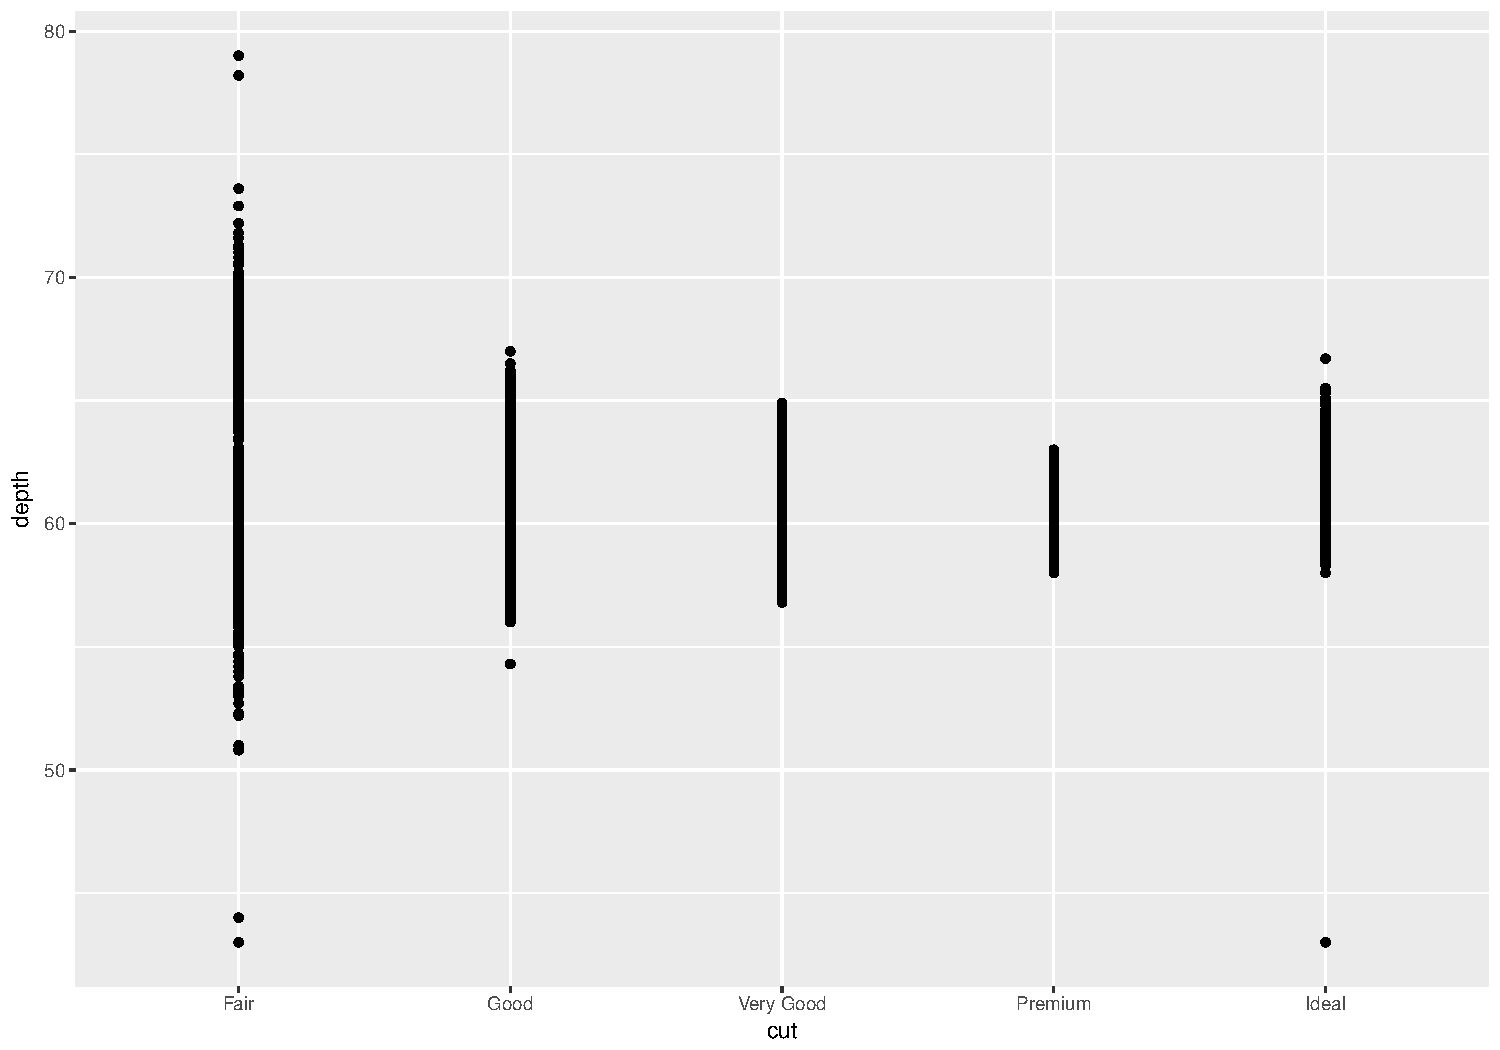
\includegraphics{RSocialScience2_files/figure-beamer/unnamed-chunk-10-1.pdf}

\end{frame}

\begin{frame}[fragile]{Ein Balkendiagramm}

\begin{Shaded}
\begin{Highlighting}[]
\KeywordTok{qplot}\NormalTok{(cut, depth, }\DataTypeTok{data=}\NormalTok{diamonds2)}
\end{Highlighting}
\end{Shaded}

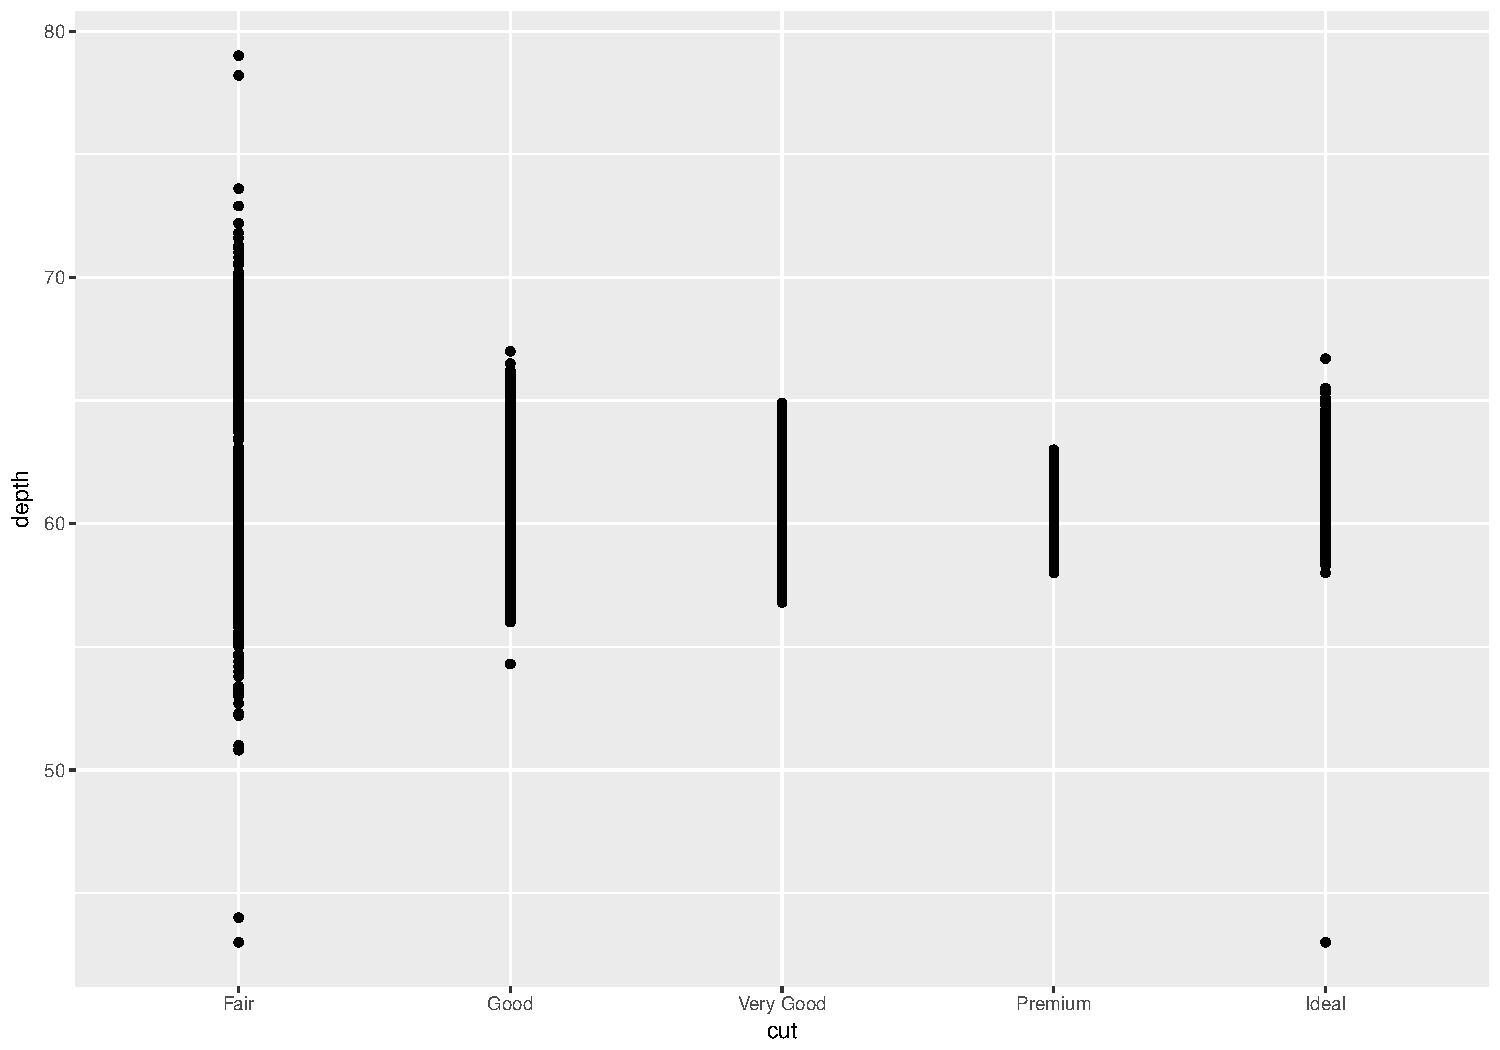
\includegraphics{RSocialScience2_files/figure-beamer/unnamed-chunk-11-1.pdf}

\end{frame}

\begin{frame}[fragile]{Ein weiteres Balkendiagramm}

\begin{Shaded}
\begin{Highlighting}[]
\KeywordTok{qplot}\NormalTok{(}\KeywordTok{factor}\NormalTok{(cyl), }\DataTypeTok{data=}\NormalTok{mtcars,}\DataTypeTok{geom=}\StringTok{"bar"}\NormalTok{)}
\end{Highlighting}
\end{Shaded}

\begin{figure}[htbp]
\centering
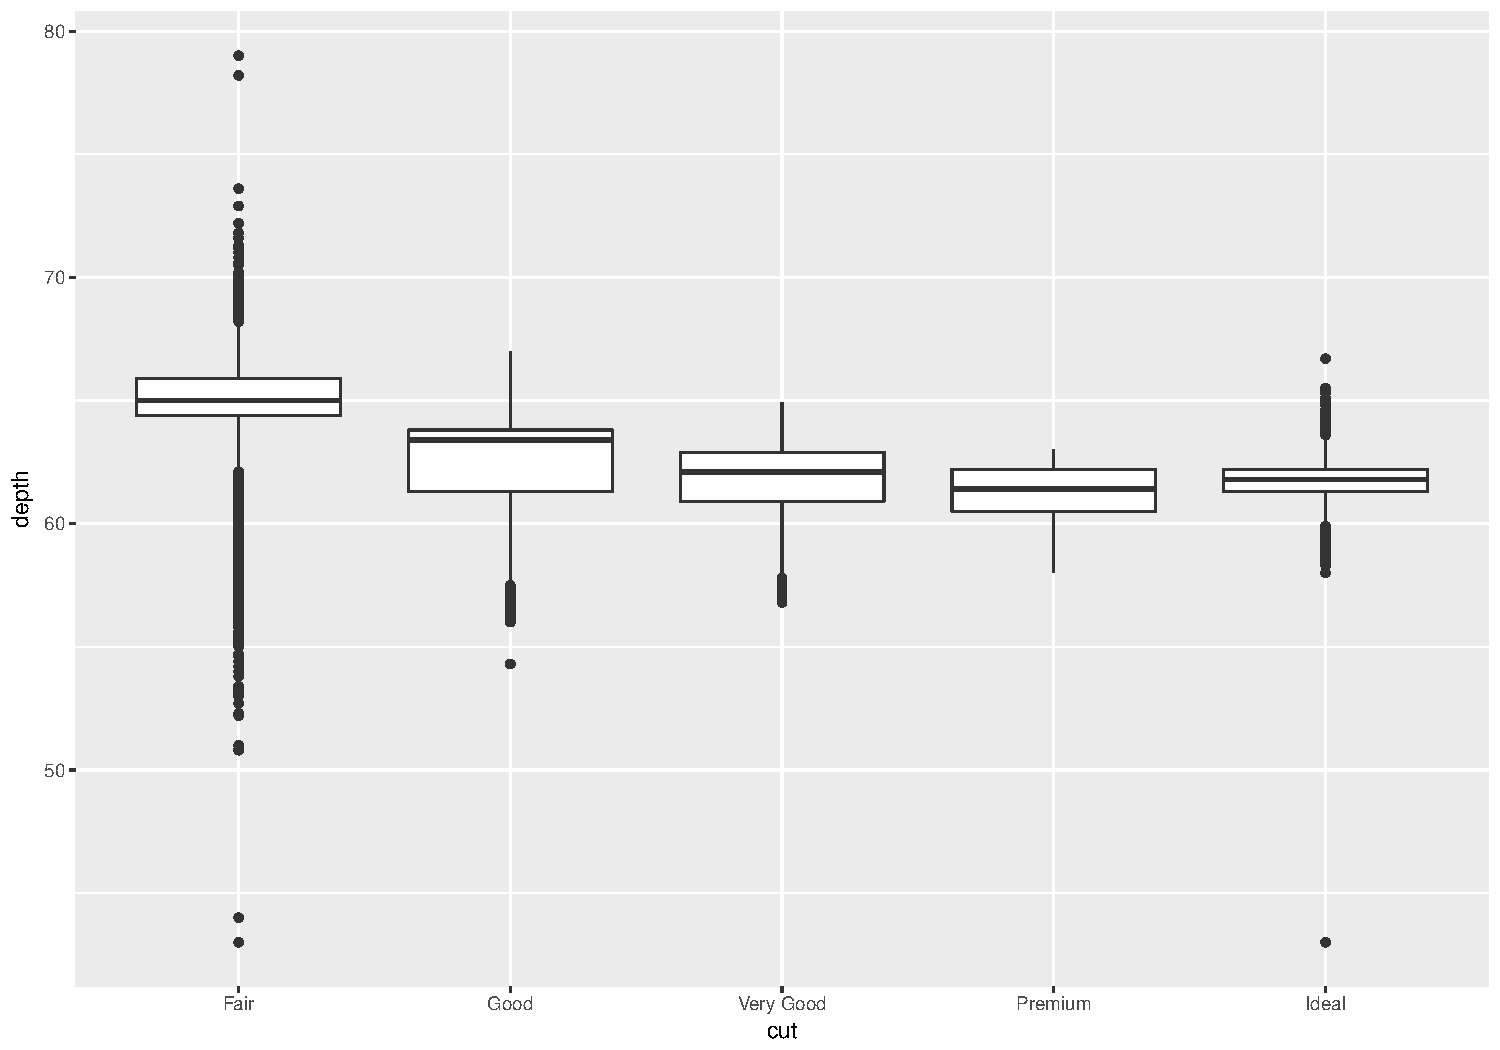
\includegraphics{RSocialScience2_files/figure-beamer/unnamed-chunk-12-1.pdf}
\caption{}
\end{figure}

\end{frame}

\begin{frame}[fragile]{Boxplot}

\begin{Shaded}
\begin{Highlighting}[]
\KeywordTok{qplot}\NormalTok{(}\DataTypeTok{data=}\NormalTok{diamonds2,}\DataTypeTok{x=}\NormalTok{cut,}\DataTypeTok{y=}\NormalTok{depth,}\DataTypeTok{geom=}\StringTok{"boxplot"}\NormalTok{)}
\end{Highlighting}
\end{Shaded}

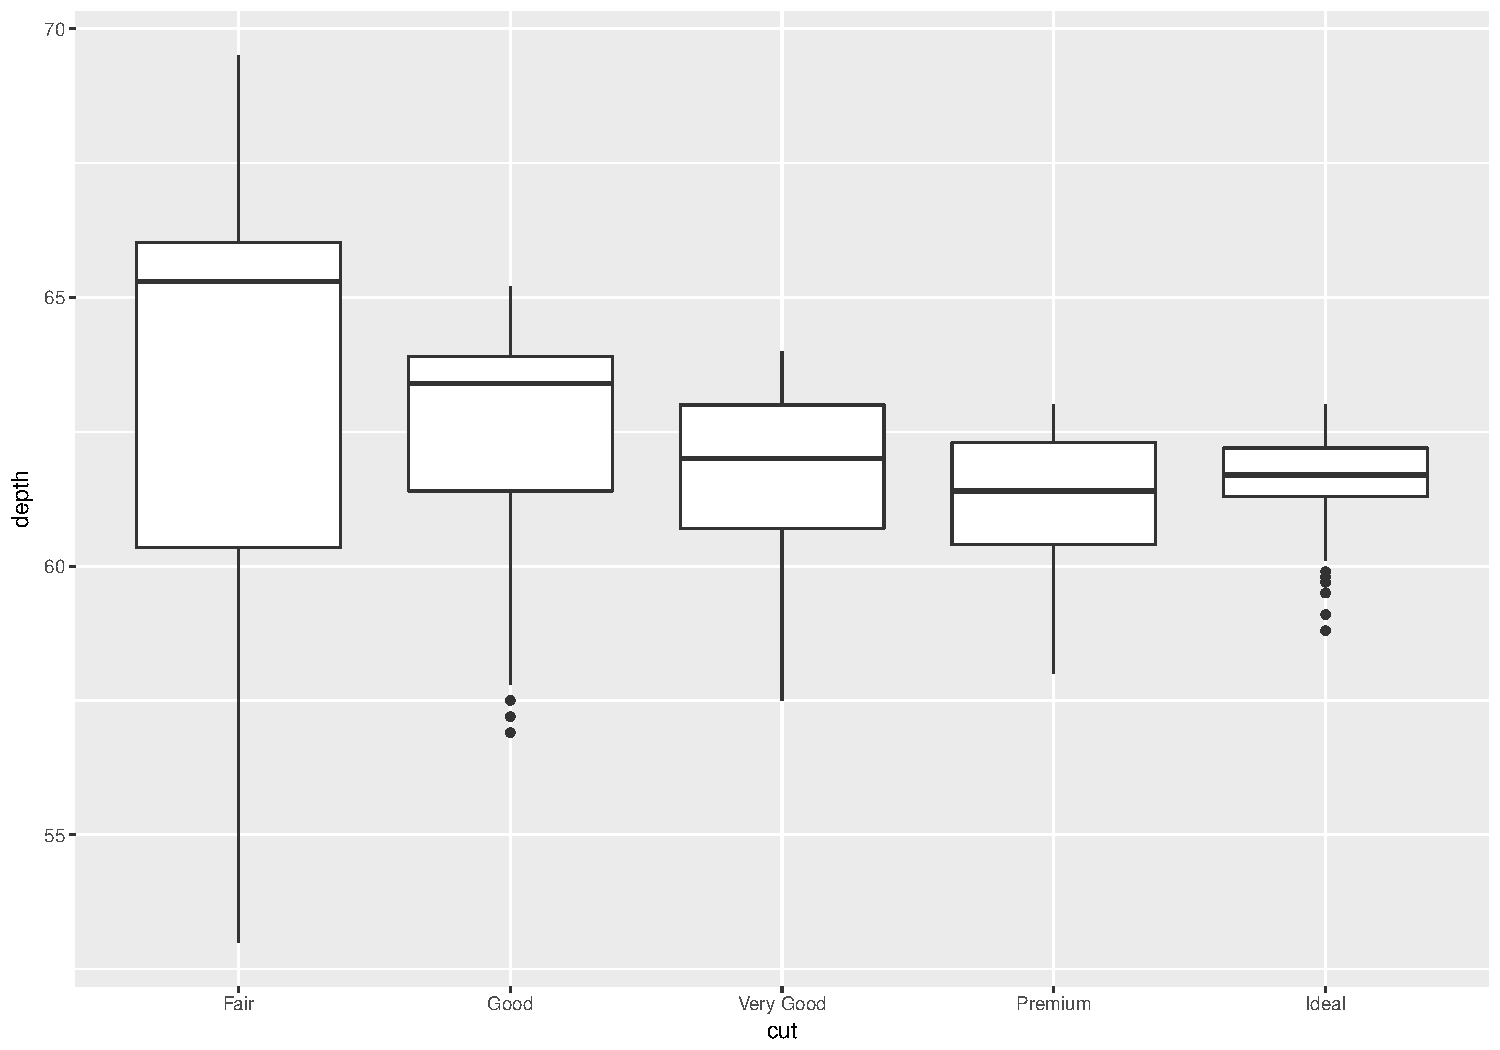
\includegraphics{RSocialScience2_files/figure-beamer/unnamed-chunk-13-1.pdf}

\end{frame}

\begin{frame}[fragile]{Scatterplot}

\begin{Shaded}
\begin{Highlighting}[]
\CommentTok{# scatterplot}
\KeywordTok{qplot}\NormalTok{(carat, depth, }\DataTypeTok{data=}\NormalTok{diamonds2)}
\end{Highlighting}
\end{Shaded}

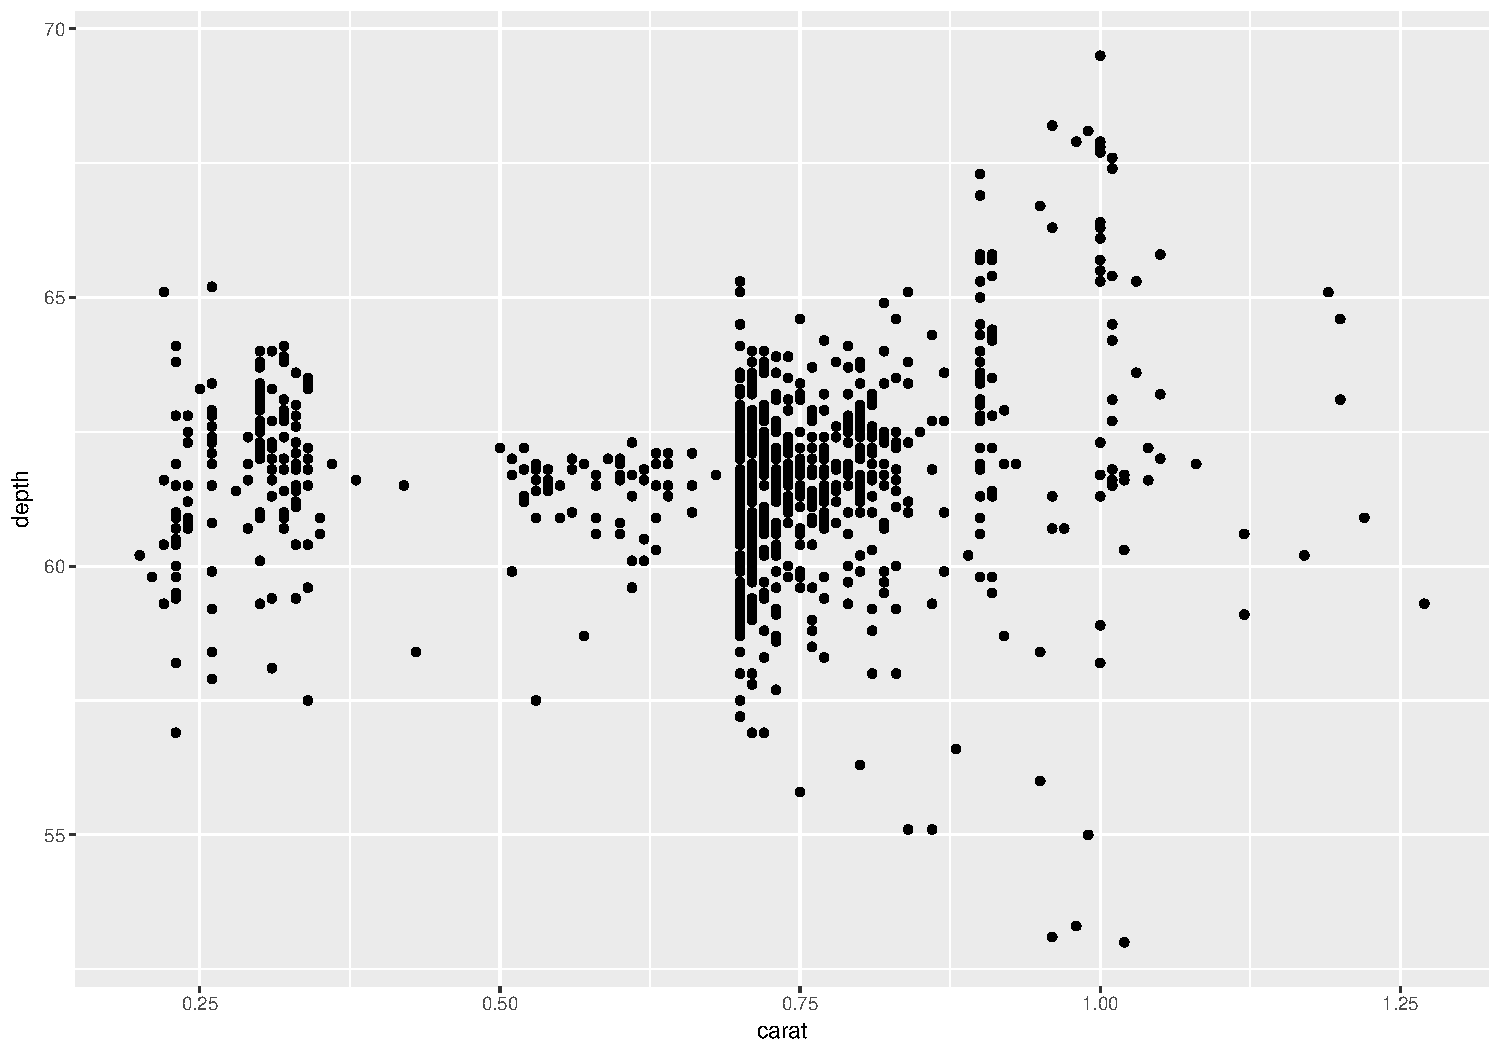
\includegraphics{RSocialScience2_files/figure-beamer/unnamed-chunk-14-1.pdf}

\end{frame}

\begin{frame}[fragile]{Farbe hinzu:}

\begin{Shaded}
\begin{Highlighting}[]
\KeywordTok{qplot}\NormalTok{(carat, depth, }\DataTypeTok{data=}\NormalTok{diamonds2,}\DataTypeTok{color=}\NormalTok{cut)}
\end{Highlighting}
\end{Shaded}

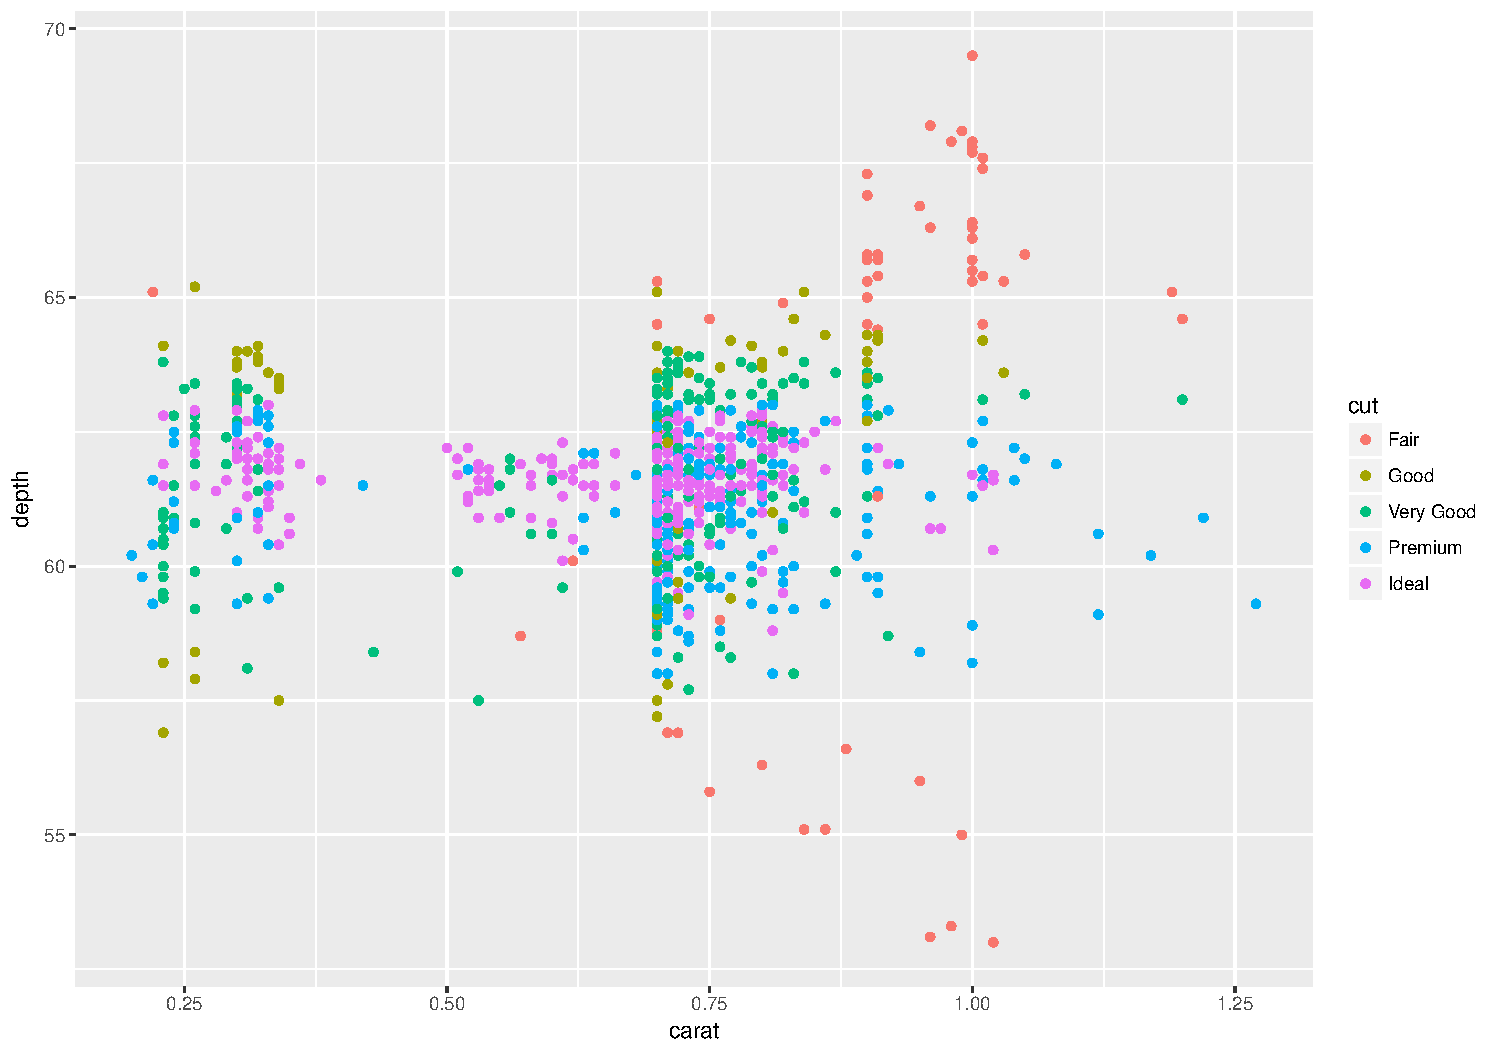
\includegraphics{RSocialScience2_files/figure-beamer/unnamed-chunk-15-1.pdf}

\end{frame}

\begin{frame}[fragile]{Trendlinie hinzufügen}

\begin{Shaded}
\begin{Highlighting}[]
\NormalTok{myGG<-}\KeywordTok{qplot}\NormalTok{(}\DataTypeTok{data=}\NormalTok{diamonds2,}\DataTypeTok{x=}\NormalTok{carat,}\DataTypeTok{y=}\NormalTok{depth,}\DataTypeTok{color=}\NormalTok{carat) }
\NormalTok{myGG +}\StringTok{ }\KeywordTok{stat_smooth}\NormalTok{(}\DataTypeTok{method=}\StringTok{"lm"}\NormalTok{)}
\end{Highlighting}
\end{Shaded}

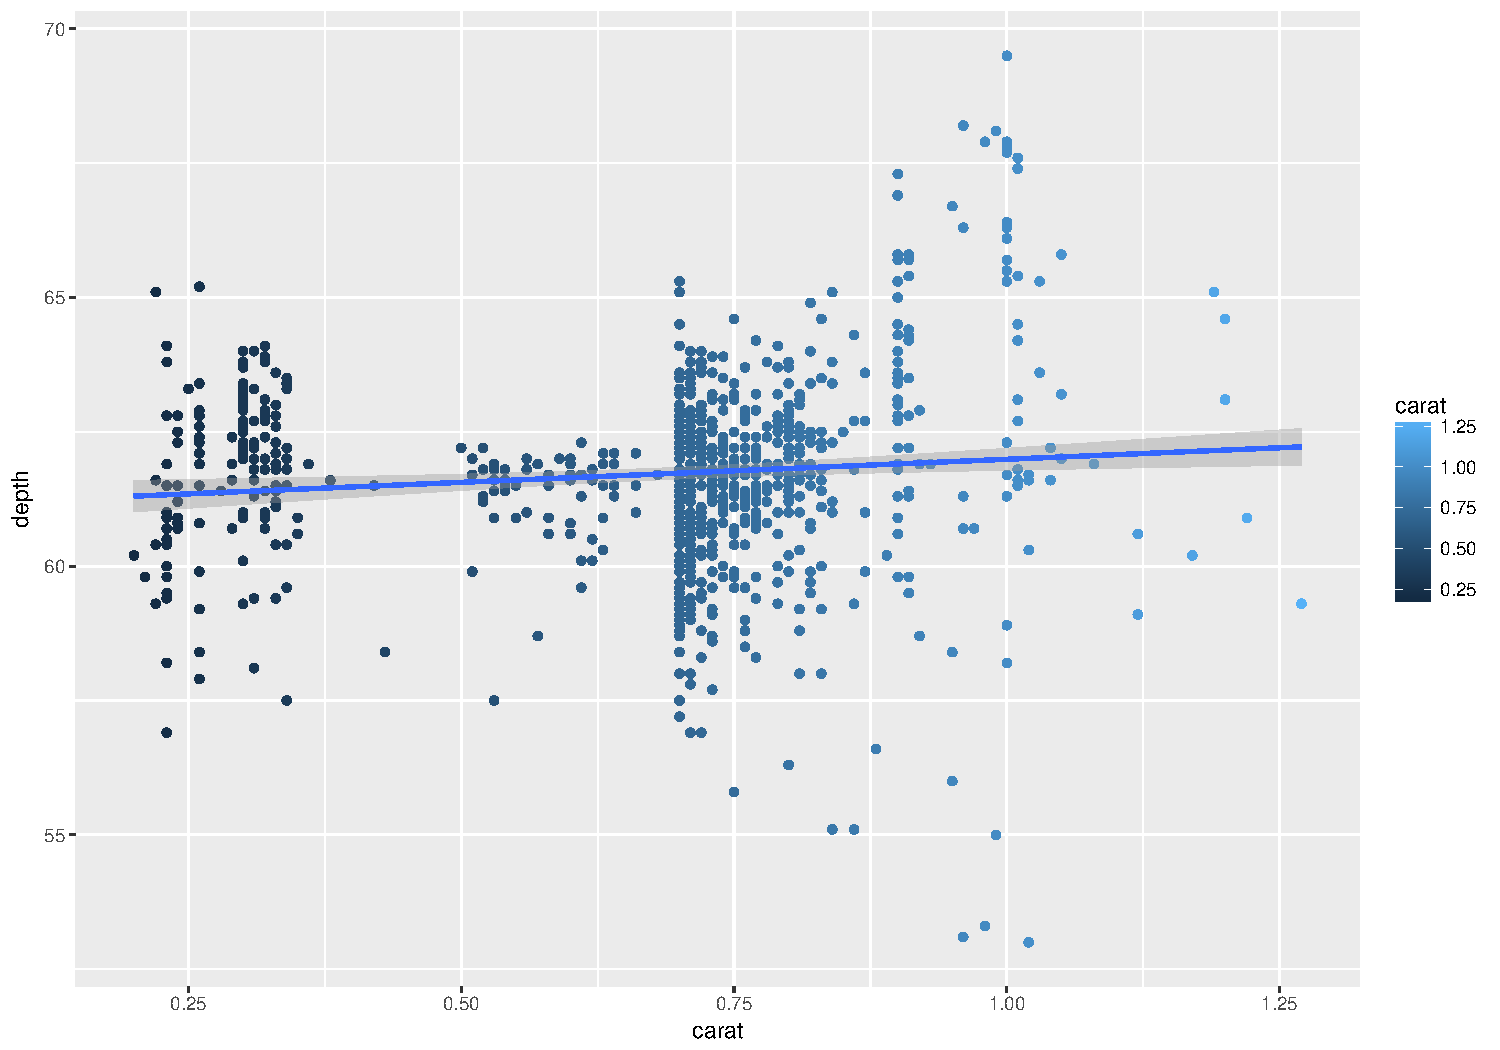
\includegraphics{RSocialScience2_files/figure-beamer/unnamed-chunk-16-1.pdf}

\end{frame}

\begin{frame}[fragile]{Graphik drehen}

\begin{Shaded}
\begin{Highlighting}[]
\KeywordTok{qplot}\NormalTok{(}\KeywordTok{factor}\NormalTok{(cyl), }\DataTypeTok{data=}\NormalTok{mtcars, }\DataTypeTok{geom=}\StringTok{"bar"}\NormalTok{) +}\StringTok{ }
\KeywordTok{coord_flip}\NormalTok{()}
\end{Highlighting}
\end{Shaded}

\begin{figure}[htbp]
\centering
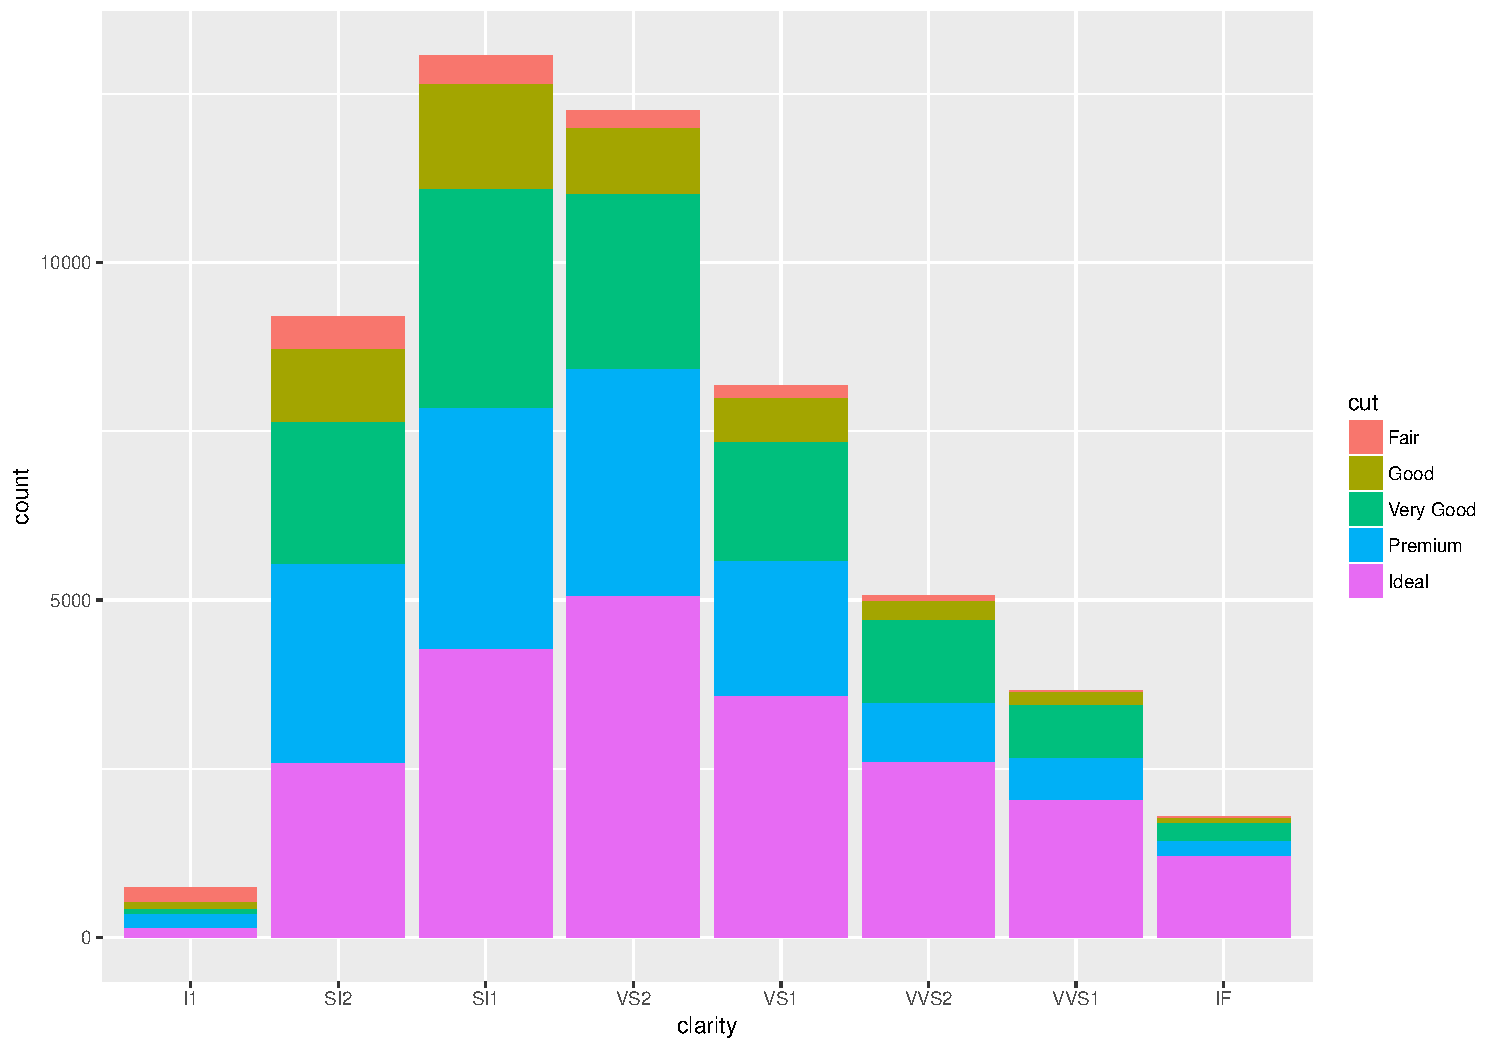
\includegraphics{RSocialScience2_files/figure-beamer/unnamed-chunk-17-1.pdf}
\caption{}
\end{figure}

\end{frame}

\begin{frame}[fragile]{Wie nutzt man ggplot}

\begin{itemize}
\tightlist
\item
  die aestetics:
\end{itemize}

\begin{Shaded}
\begin{Highlighting}[]
\KeywordTok{ggplot}\NormalTok{(diamonds2, }\KeywordTok{aes}\NormalTok{(clarity, }\DataTypeTok{fill=}\NormalTok{cut)) +}\StringTok{ }\KeywordTok{geom_bar}\NormalTok{()}
\end{Highlighting}
\end{Shaded}

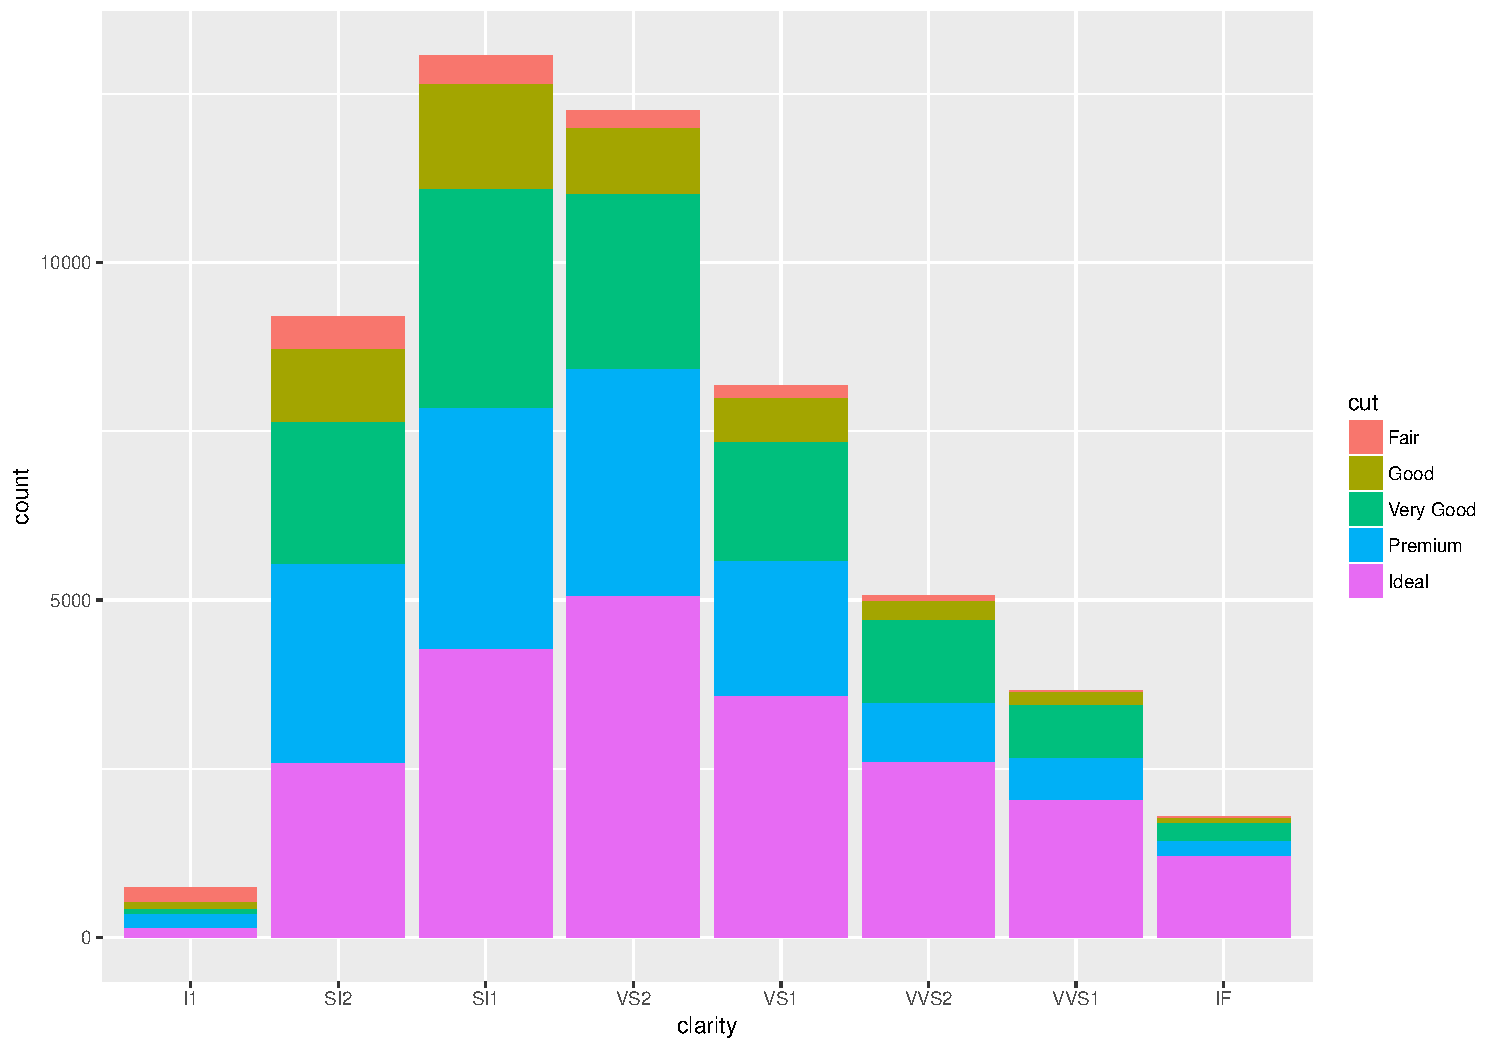
\includegraphics{RSocialScience2_files/figure-beamer/unnamed-chunk-18-1.pdf}

\end{frame}

\begin{frame}[fragile]{Farben selber wählen}

Es wird das Paket \texttt{RColorBrewer} verwendet um die Farbpalette zu
ändern

\begin{Shaded}
\begin{Highlighting}[]
\KeywordTok{install.packages}\NormalTok{(}\StringTok{"RColorBrewer"}\NormalTok{)}
\end{Highlighting}
\end{Shaded}

\begin{Shaded}
\begin{Highlighting}[]
\KeywordTok{library}\NormalTok{(RColorBrewer)}
\NormalTok{myColors <-}\StringTok{ }\KeywordTok{brewer.pal}\NormalTok{(}\DecValTok{5}\NormalTok{,}\StringTok{"Accent"}\NormalTok{)}
\KeywordTok{names}\NormalTok{(myColors) <-}\StringTok{ }\KeywordTok{levels}\NormalTok{(diamonds2$cut)}
\NormalTok{colScale <-}\StringTok{ }\KeywordTok{scale_colour_manual}\NormalTok{(}\DataTypeTok{name =} \StringTok{"cut"}\NormalTok{,}
                                \DataTypeTok{values =} \NormalTok{myColors)}
\end{Highlighting}
\end{Shaded}

\url{http://stackoverflow.com/questions/6919025/}

\end{frame}

\begin{frame}[fragile]{Eine Graphik mit den gewählten Farben}

\begin{Shaded}
\begin{Highlighting}[]
\NormalTok{p <-}\StringTok{ }\KeywordTok{ggplot}\NormalTok{(diamonds2,}\KeywordTok{aes}\NormalTok{(carat, depth,}\DataTypeTok{colour =} \NormalTok{cut)) +}\StringTok{ }
\StringTok{  }\KeywordTok{geom_point}\NormalTok{()}
\NormalTok{p +}\StringTok{ }\NormalTok{colScale}
\end{Highlighting}
\end{Shaded}

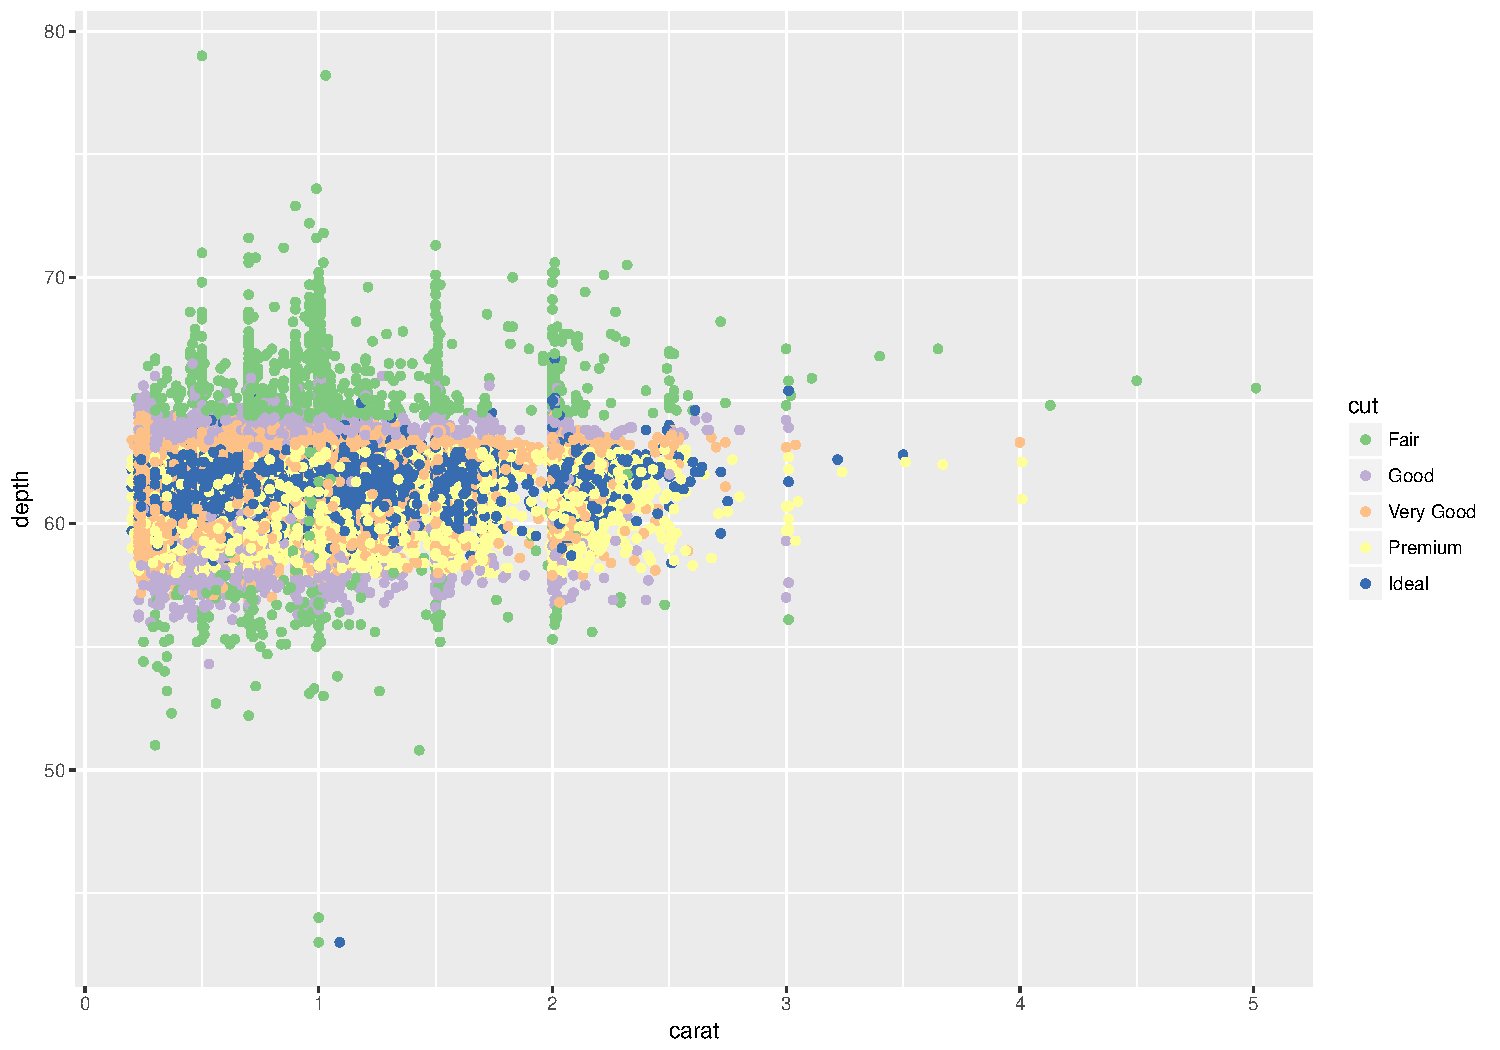
\includegraphics{RSocialScience2_files/figure-beamer/unnamed-chunk-21-1.pdf}

\end{frame}

\begin{frame}[fragile]{Speichern mit ggsave}

\begin{Shaded}
\begin{Highlighting}[]
\KeywordTok{ggsave}\NormalTok{(}\StringTok{"Graphik.jpg"}\NormalTok{)}
\end{Highlighting}
\end{Shaded}

\end{frame}

\begin{frame}{Links}

\begin{itemize}
\tightlist
\item
  \href{http://www.r-bloggers.com/why-i-use-ggplot2/}{Warum man ggplot2
  für einfache Grafiken nutzen sollte}
\end{itemize}

\begin{figure}[htbp]
\centering
\includegraphics{https://github.com/Japhilko/IntroR/raw/master/2017/slides/figure/WhyIuseggplot2.PNG}
\caption{}
\end{figure}

\begin{itemize}
\tightlist
\item
  \href{https://opr.princeton.edu/workshops/Downloads/2015Jan_ggplot2Koffman.pdf}{Einführung
  in ggplot2}
\end{itemize}

\includegraphics{https://github.com/Japhilko/IntroR/raw/master/2017/slides/figure/introggplot2.PNG}
-
\href{http://tutorials.iq.harvard.edu/R/Rgraphics/Rgraphics.html}{ggplot2
Basics}

\begin{itemize}
\item
  Noam Ross -
  \href{http://www.noamross.net/blog/2012/10/5/ggplot-introduction.html}{Quick
  Introduction to ggplot2}
\item
  \href{https://www.r-bloggers.com/rcmdrplugin-kmggplot2_0-2-4-is-on-cran/}{Plugin
  ggplot2}
\end{itemize}

\end{frame}

\begin{frame}{Verschiedene Kartentypen}

Arten von räumlichen Daten:

\begin{itemize}
\tightlist
\item
  \href{https://www.nceas.ucsb.edu/~frazier/RSpatialGuides/ggmap/ggmapCheatsheet.pdf}{Straßenkarten}
\item
  \href{http://www.mostlymuppet.com/tag/maps/}{Satelliten Bilder}
\item
  \href{http://gis.stackexchange.com/questions/3083/what-makes-a-map-beautiful/45518\#45518}{Physische
  Daten und Karten}
\item
  \href{http://www.designfaves.com/2014/03/abstracted-maps-reveal-cities-personalities}{Abstrakte
  Karten}
\item
  \ldots{}
\end{itemize}

Das R-paket
\href{http://journal.r-project.org/archive/2013-1/kahle-wickham.pdf}{ggmap}
wird im folgenden genutzt um verschiedene Kartentypen darzustellen.

Mit \href{http://www.inside-r.org/packages/cran/ggmap/docs/qmap}{qmap}
kann man eine schnelle Karte erzeugen.

\end{frame}

\begin{frame}{Straßenkarten}

\begin{itemize}
\tightlist
\item
  Straßenkarte werden sehr häufig verwendet.
\item
  Diese Karten zeigen Haupt- und Nebenstraßen (abhängig vom Detail)
\item
  oft sind auch weitere Informationen enthalten. Wie beispielsweise
  Flughäfen, Städte, Campingplätze oder andere Orte von Interesse
\item
  Beispiel einer Straßenkarte für
  \href{http://rpubs.com/Japhilko82/OpenStreetMap_Mannheim}{Mannheim}.
\end{itemize}

\end{frame}

\begin{frame}[fragile]{Installieren des Paketes}

\begin{itemize}
\tightlist
\item
  Zur Erstellung der Karten brauchen wir das Paket \texttt{ggmap}:
\end{itemize}

\begin{Shaded}
\begin{Highlighting}[]
\NormalTok{devtools::}\KeywordTok{install_github}\NormalTok{(}\StringTok{"dkahle/ggmap"}\NormalTok{)}
\NormalTok{devtools::}\KeywordTok{install_github}\NormalTok{(}\StringTok{"hadley/ggplot2"}\NormalTok{)}
\KeywordTok{install.packages}\NormalTok{(}\StringTok{"ggmap"}\NormalTok{)}
\end{Highlighting}
\end{Shaded}

\end{frame}

\begin{frame}[fragile]{Paket ggmap - Hallo Welt}

\begin{itemize}
\tightlist
\item
  Um das Paket zu laden verwenden wir den Befehl \texttt{library}
\end{itemize}

\begin{Shaded}
\begin{Highlighting}[]
\KeywordTok{library}\NormalTok{(ggmap)}
\end{Highlighting}
\end{Shaded}

Und schon kann die erste Karte erstellt werden:

\begin{Shaded}
\begin{Highlighting}[]
\KeywordTok{qmap}\NormalTok{(}\StringTok{"Mannheim"}\NormalTok{)}
\end{Highlighting}
\end{Shaded}

\begin{figure}[htbp]
\centering
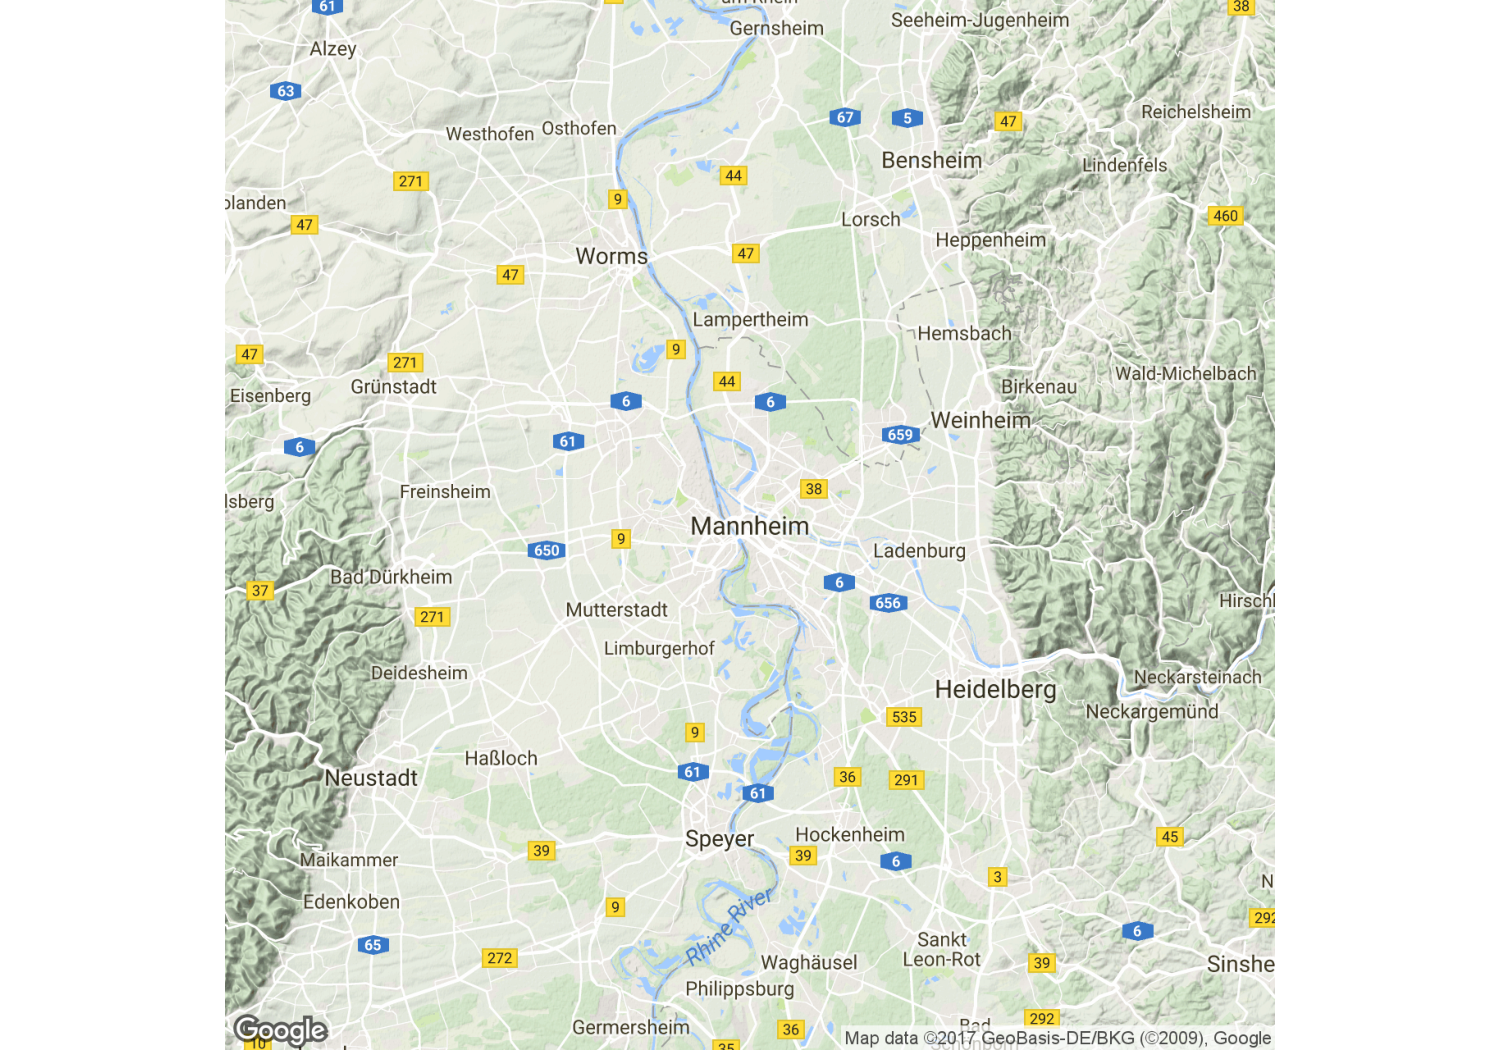
\includegraphics{RSocialScience2_files/figure-beamer/unnamed-chunk-26-1.pdf}
\caption{}
\end{figure}

\end{frame}

\begin{frame}[fragile]{Karte für eine Sehenswürdigkeit}

\begin{Shaded}
\begin{Highlighting}[]
\NormalTok{BBT <-}\StringTok{ }\KeywordTok{qmap}\NormalTok{(}\StringTok{"Berlin Brandenburger Tor"}\NormalTok{)}
\NormalTok{BBT}
\end{Highlighting}
\end{Shaded}

\begin{figure}[htbp]
\centering
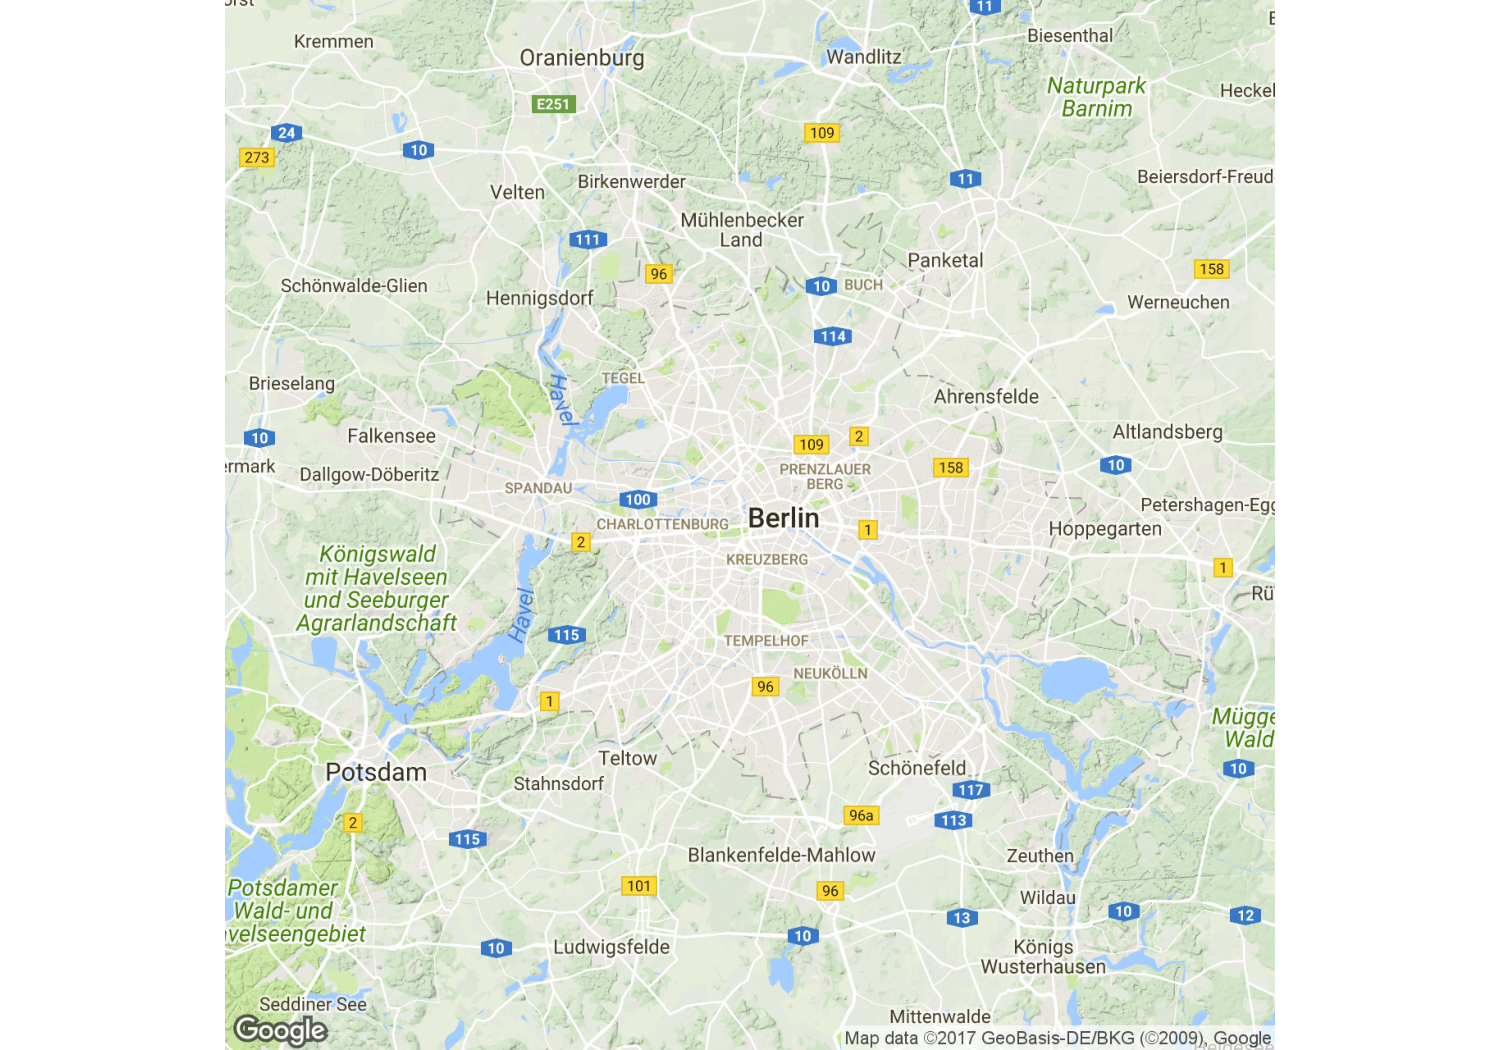
\includegraphics{RSocialScience2_files/figure-beamer/unnamed-chunk-28-1.pdf}
\caption{}
\end{figure}

\end{frame}

\begin{frame}[fragile]{Karte für einen ganzen Staat}

\begin{Shaded}
\begin{Highlighting}[]
\KeywordTok{qmap}\NormalTok{(}\StringTok{"Germany"}\NormalTok{)}
\end{Highlighting}
\end{Shaded}

\begin{figure}[htbp]
\centering
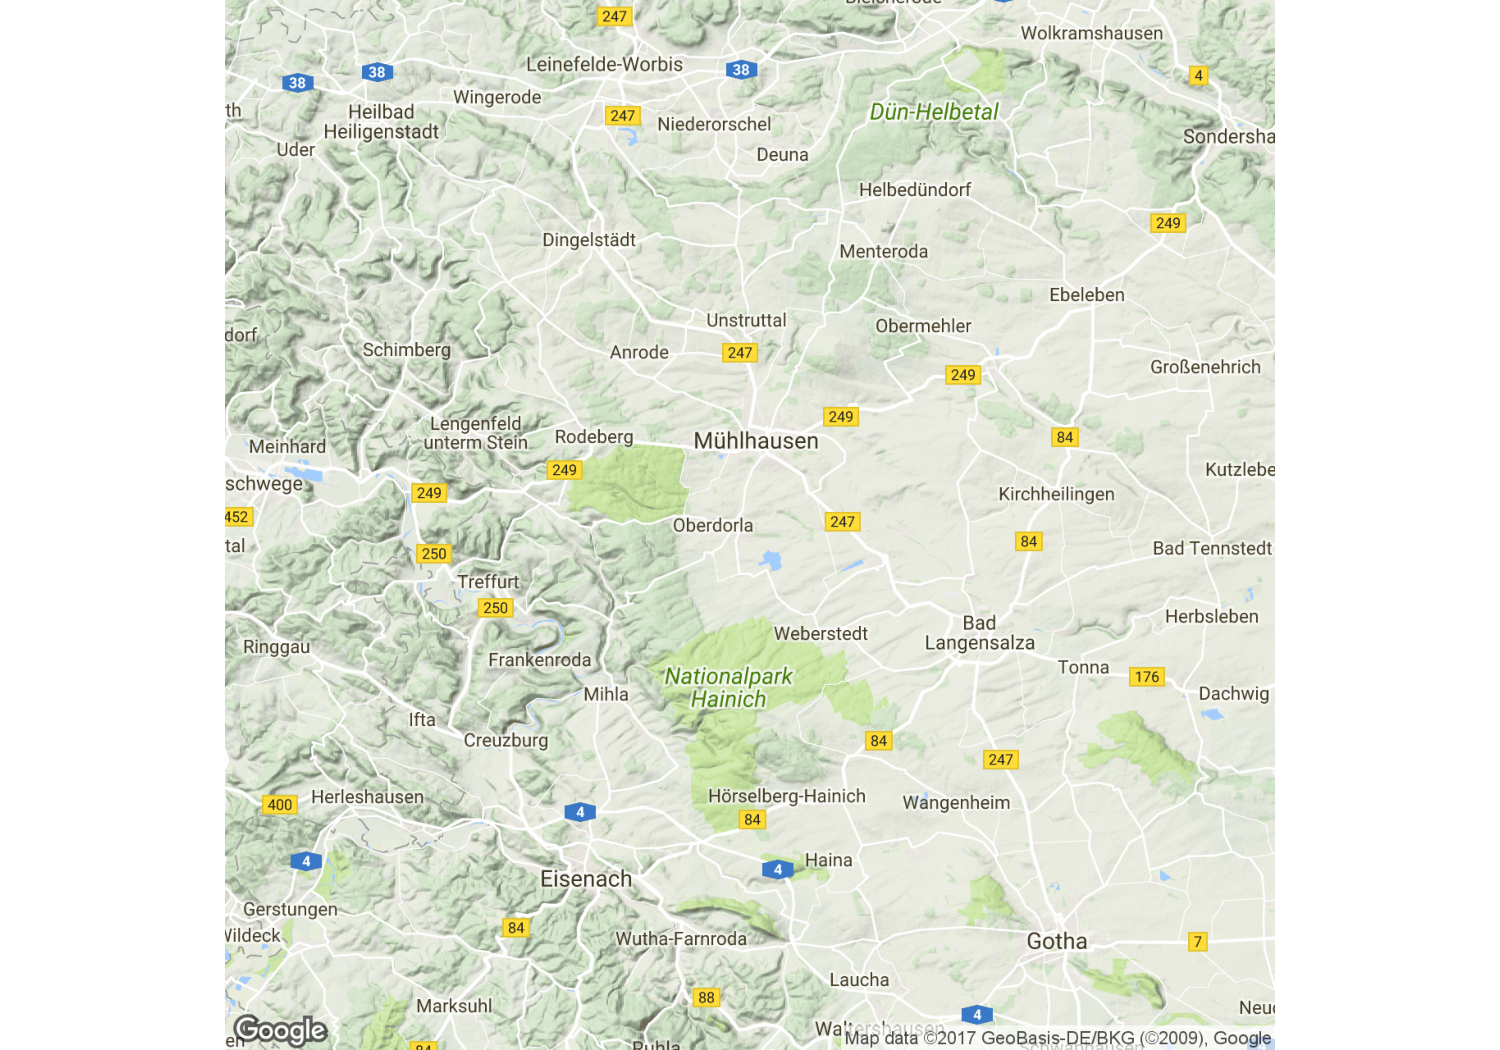
\includegraphics{RSocialScience2_files/figure-beamer/unnamed-chunk-29-1.pdf}
\caption{}
\end{figure}

\begin{itemize}
\tightlist
\item
  Wir brauchen ein anderes \emph{zoom level}
\end{itemize}

\end{frame}

\begin{frame}[fragile]{Ein anderes \emph{zoom level}}

\begin{itemize}
\tightlist
\item
  level 3 - Kontinent
\item
  level 10 - Stadt
\item
  level 21 - Gebäude
\end{itemize}

\begin{Shaded}
\begin{Highlighting}[]
\KeywordTok{qmap}\NormalTok{(}\StringTok{"Germany"}\NormalTok{, }\DataTypeTok{zoom =} \DecValTok{6}\NormalTok{)}
\end{Highlighting}
\end{Shaded}

\begin{figure}[htbp]
\centering
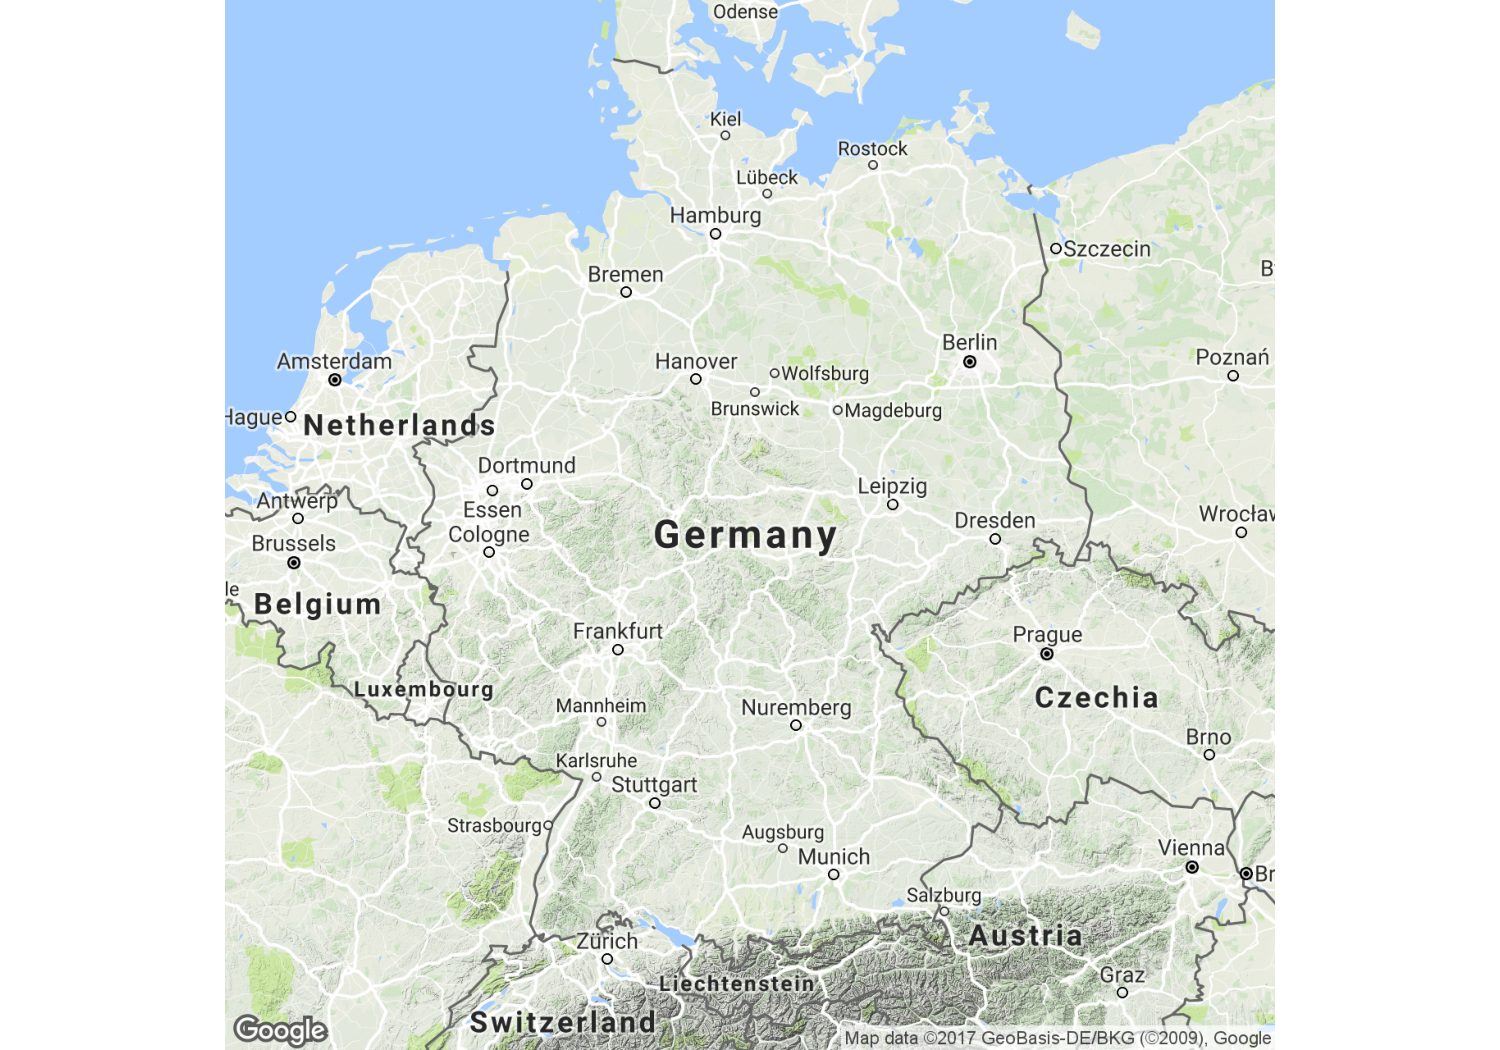
\includegraphics{RSocialScience2_files/figure-beamer/unnamed-chunk-30-1.pdf}
\caption{}
\end{figure}

\end{frame}

\begin{frame}[fragile]{Hilfe bekommen wir mit dem Fragezeichen}

\begin{Shaded}
\begin{Highlighting}[]
\NormalTok{?qmap}
\end{Highlighting}
\end{Shaded}

Verschiedene Abschnitte in der Hilfe:

\begin{itemize}
\tightlist
\item
  Description
\item
  Usage
\item
  Arguments
\item
  Value
\item
  Author(s)
\item
  See Also
\item
  Examples
\end{itemize}

\end{frame}

\begin{frame}[fragile]{Die Beispiele in der Hilfe}

Ausschnitt aus der Hilfe Seite zum Befehl \texttt{qmap}:

\begin{figure}[htbp]
\centering
\includegraphics{https://github.com/Japhilko/IntroR/raw/master/2017/slides/figure/qmapExample.PNG}
\caption{qmap Example}
\end{figure}

Das Beispiel kann man direkt in die Konsole kopieren:

\begin{Shaded}
\begin{Highlighting}[]
\CommentTok{# qmap("baylor university")}
\KeywordTok{qmap}\NormalTok{(}\StringTok{"baylor university"}\NormalTok{, }\DataTypeTok{zoom =} \DecValTok{14}\NormalTok{)}
\end{Highlighting}
\end{Shaded}

\begin{figure}[htbp]
\centering
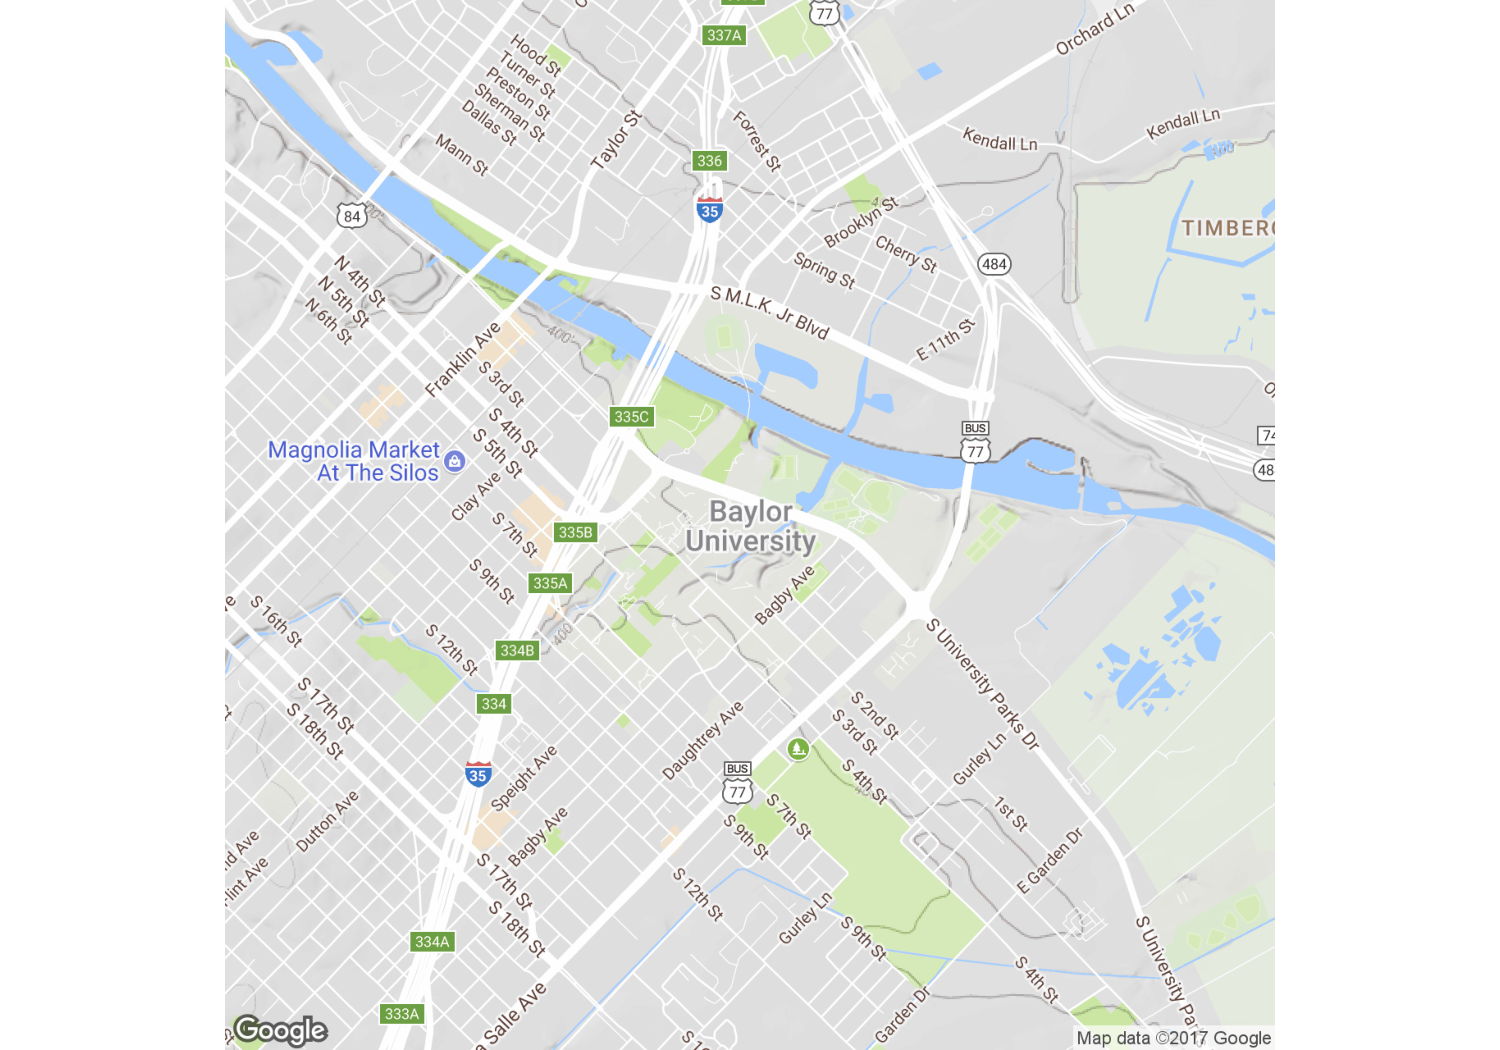
\includegraphics{RSocialScience2_files/figure-beamer/unnamed-chunk-33-1.pdf}
\caption{}
\end{figure}

\begin{Shaded}
\begin{Highlighting}[]
\CommentTok{# und so weiter}
\end{Highlighting}
\end{Shaded}

\end{frame}

\begin{frame}[fragile]{Ein anderes \emph{zoom level}}

\begin{Shaded}
\begin{Highlighting}[]
\KeywordTok{qmap}\NormalTok{(}\StringTok{"Mannheim"}\NormalTok{, }\DataTypeTok{zoom =} \DecValTok{12}\NormalTok{)}
\end{Highlighting}
\end{Shaded}

\begin{figure}[htbp]
\centering
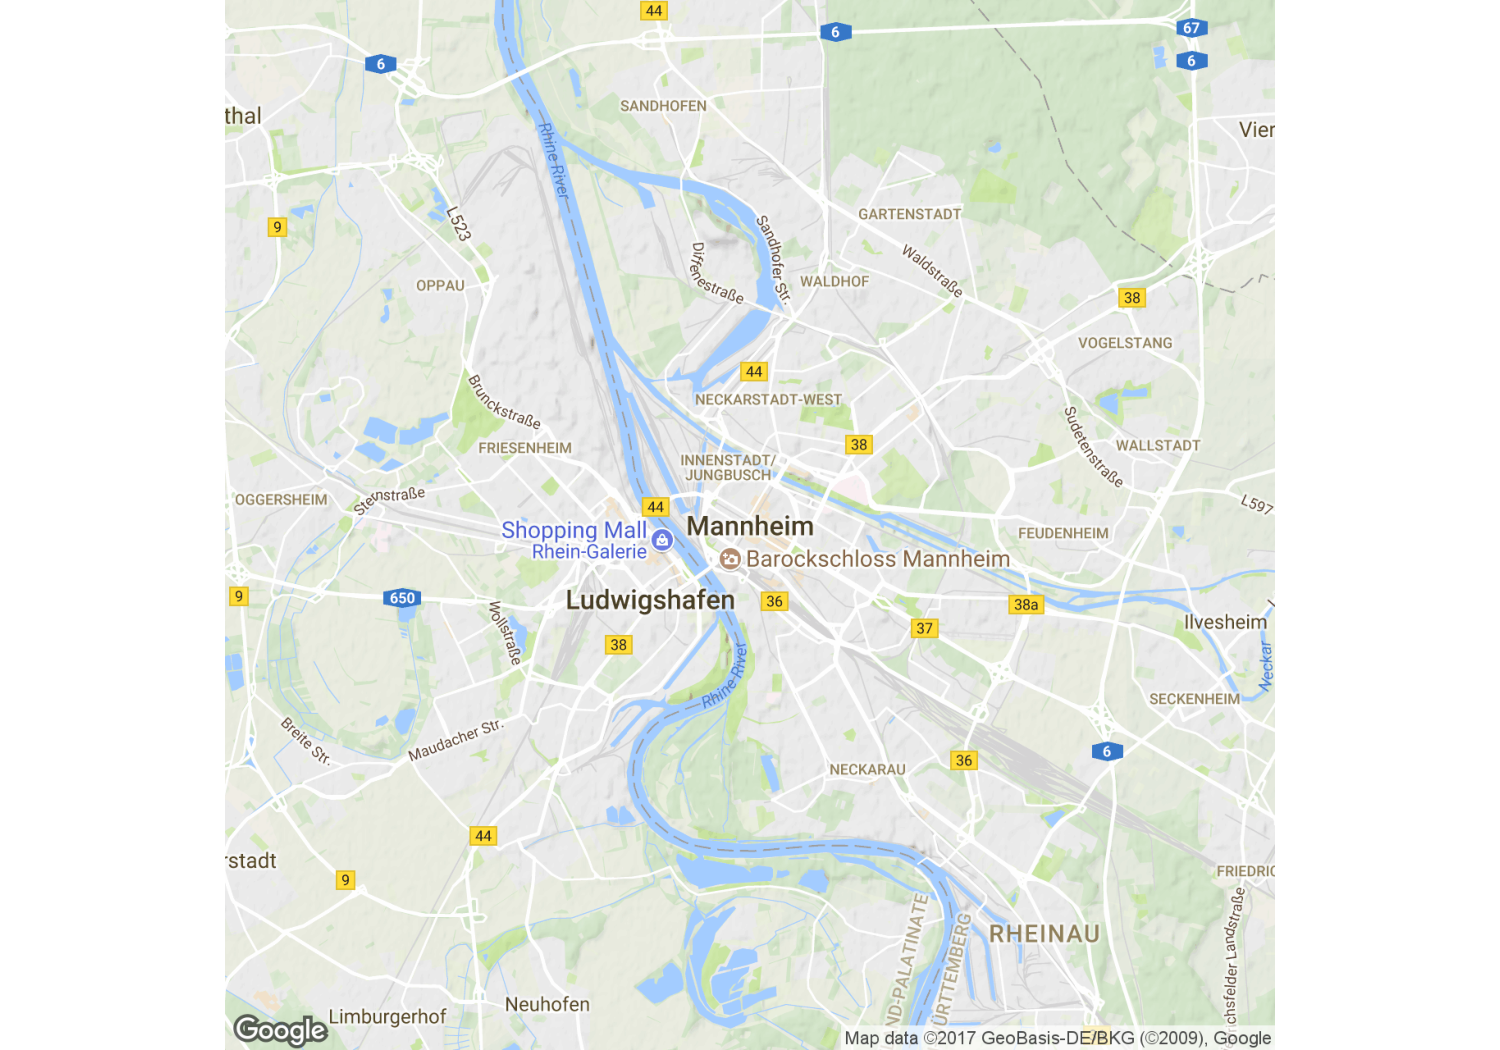
\includegraphics{RSocialScience2_files/figure-beamer/unnamed-chunk-34-1.pdf}
\caption{}
\end{figure}

\end{frame}

\begin{frame}[fragile]{Näher rankommen}

\begin{Shaded}
\begin{Highlighting}[]
\KeywordTok{qmap}\NormalTok{(}\StringTok{'Mannheim'}\NormalTok{, }\DataTypeTok{zoom =} \DecValTok{13}\NormalTok{)}
\end{Highlighting}
\end{Shaded}

\begin{figure}[htbp]
\centering
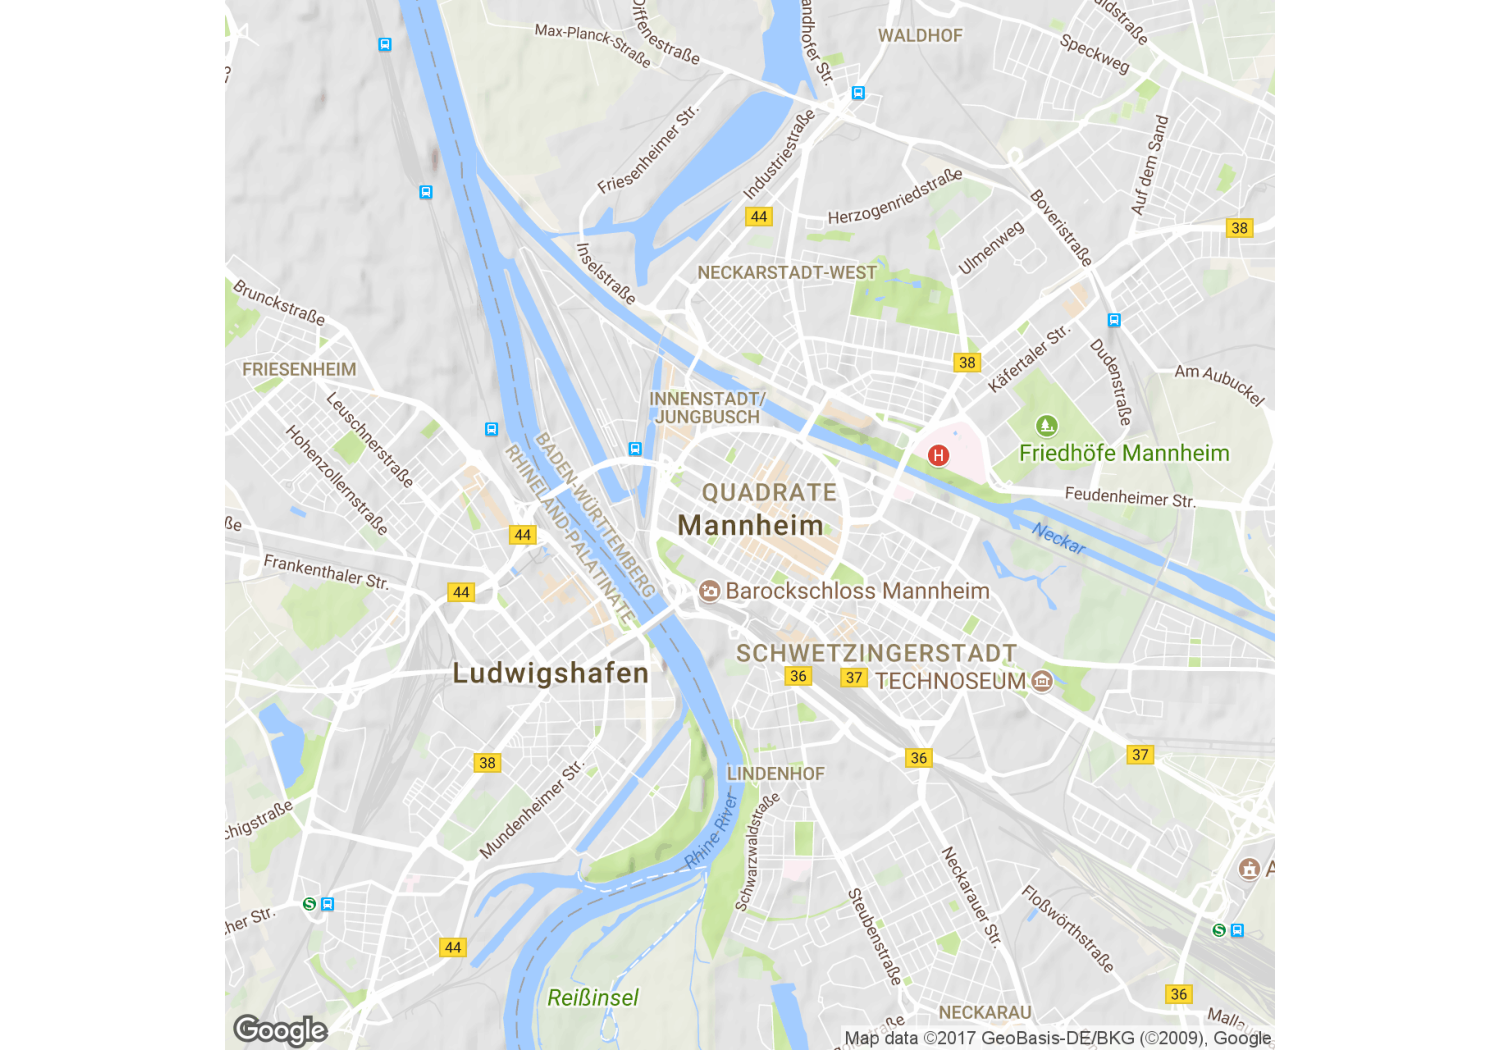
\includegraphics{RSocialScience2_files/figure-beamer/unnamed-chunk-35-1.pdf}
\caption{}
\end{figure}

\end{frame}

\begin{frame}[fragile]{Ganz nah dran}

\begin{Shaded}
\begin{Highlighting}[]
\KeywordTok{qmap}\NormalTok{(}\StringTok{'Mannheim'}\NormalTok{, }\DataTypeTok{zoom =} \DecValTok{20}\NormalTok{)}
\end{Highlighting}
\end{Shaded}

\begin{figure}[htbp]
\centering
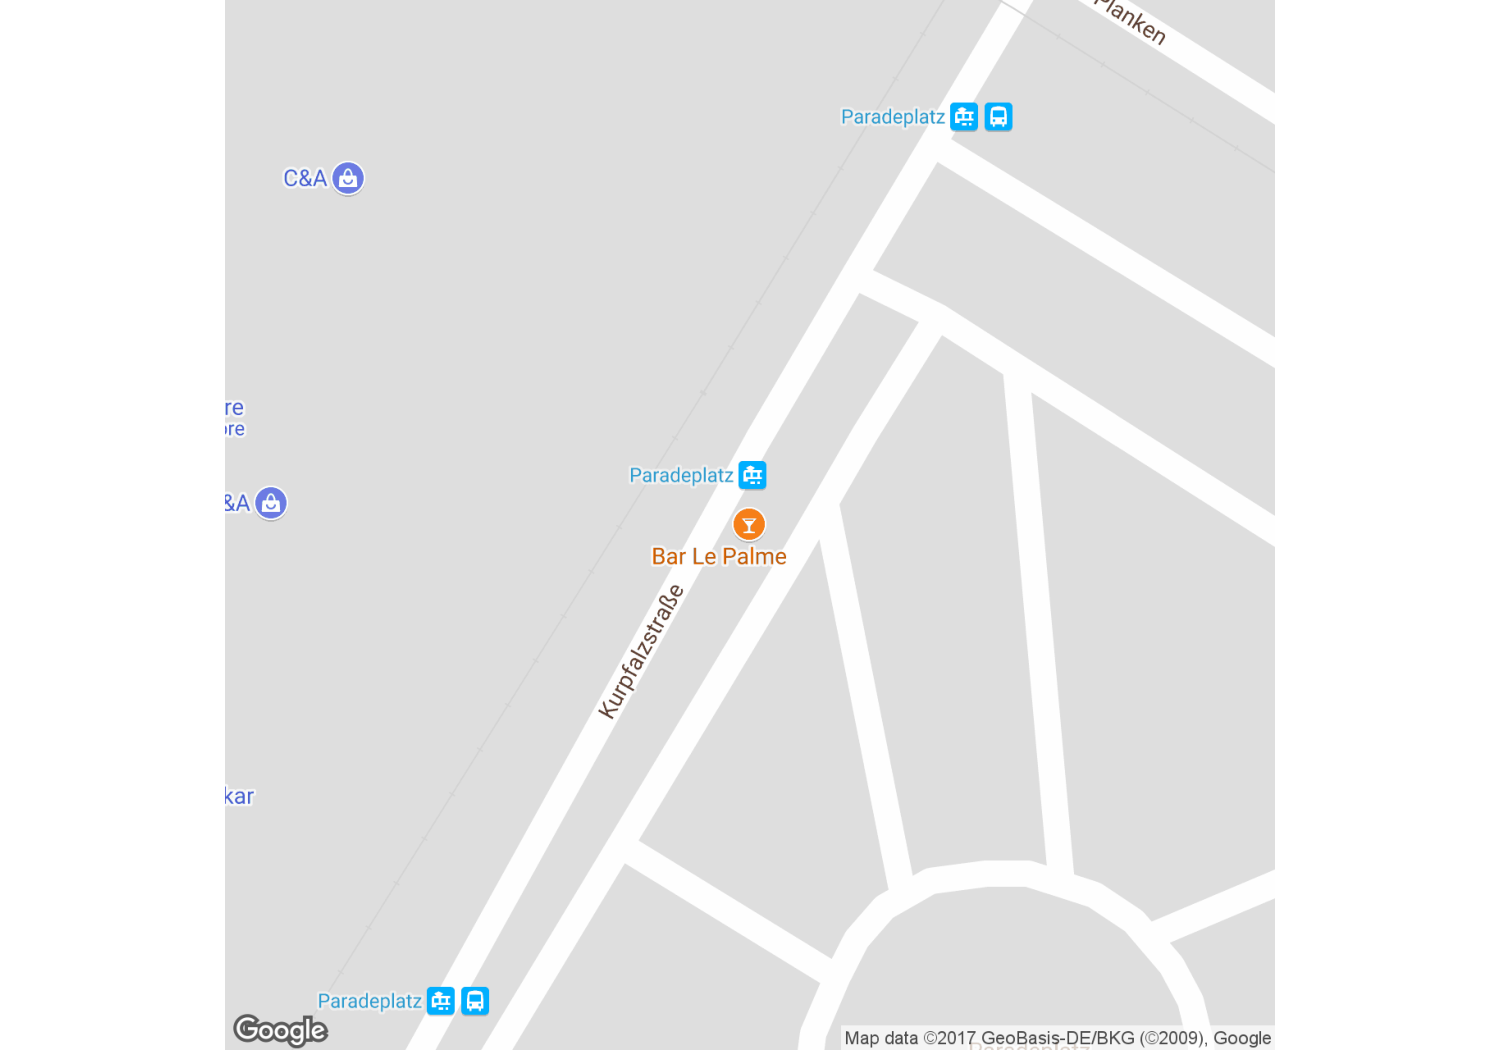
\includegraphics{RSocialScience2_files/figure-beamer/unnamed-chunk-36-1.pdf}
\caption{}
\end{figure}

\end{frame}

\begin{frame}[fragile]{ggmap - maptype satellite}

\begin{Shaded}
\begin{Highlighting}[]
\KeywordTok{qmap}\NormalTok{(}\StringTok{'Mannheim'}\NormalTok{, }\DataTypeTok{zoom =} \DecValTok{14}\NormalTok{, }\DataTypeTok{maptype=}\StringTok{"satellite"}\NormalTok{)}
\end{Highlighting}
\end{Shaded}

\begin{figure}[htbp]
\centering
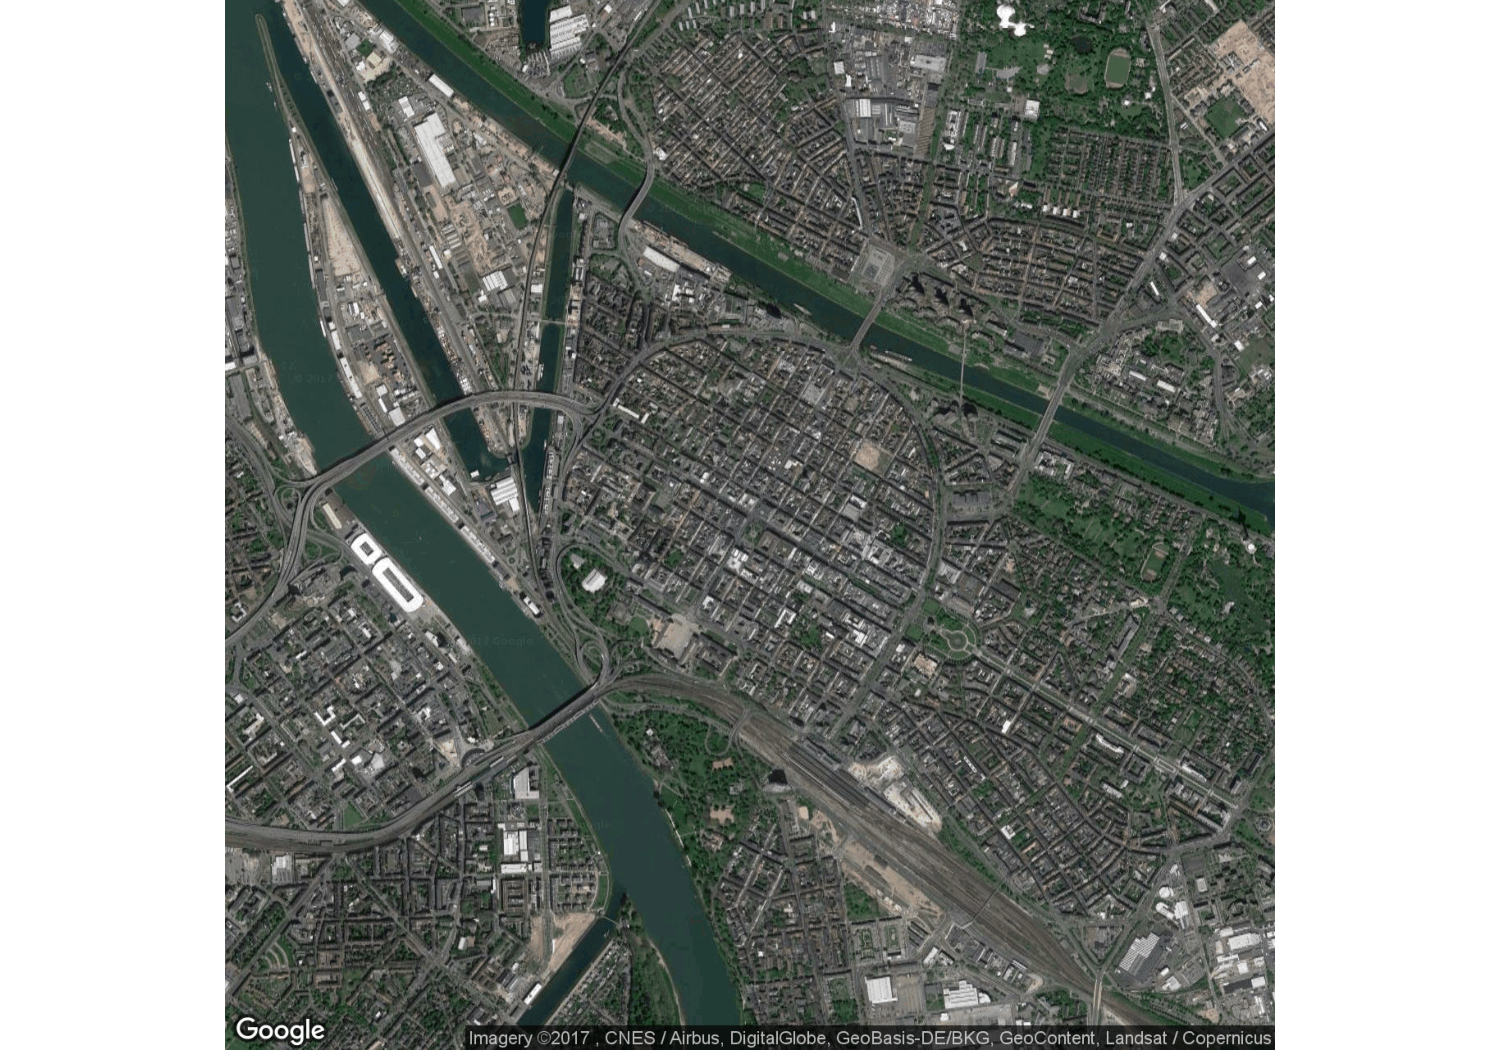
\includegraphics{RSocialScience2_files/figure-beamer/unnamed-chunk-37-1.pdf}
\caption{}
\end{figure}

\end{frame}

\begin{frame}[fragile]{ggmap - maptype satellite zoom 20}

\begin{Shaded}
\begin{Highlighting}[]
\KeywordTok{qmap}\NormalTok{(}\StringTok{'Mannheim'}\NormalTok{, }\DataTypeTok{zoom =} \DecValTok{20}\NormalTok{, }\DataTypeTok{maptype=}\StringTok{"hybrid"}\NormalTok{)}
\end{Highlighting}
\end{Shaded}

\begin{figure}[htbp]
\centering
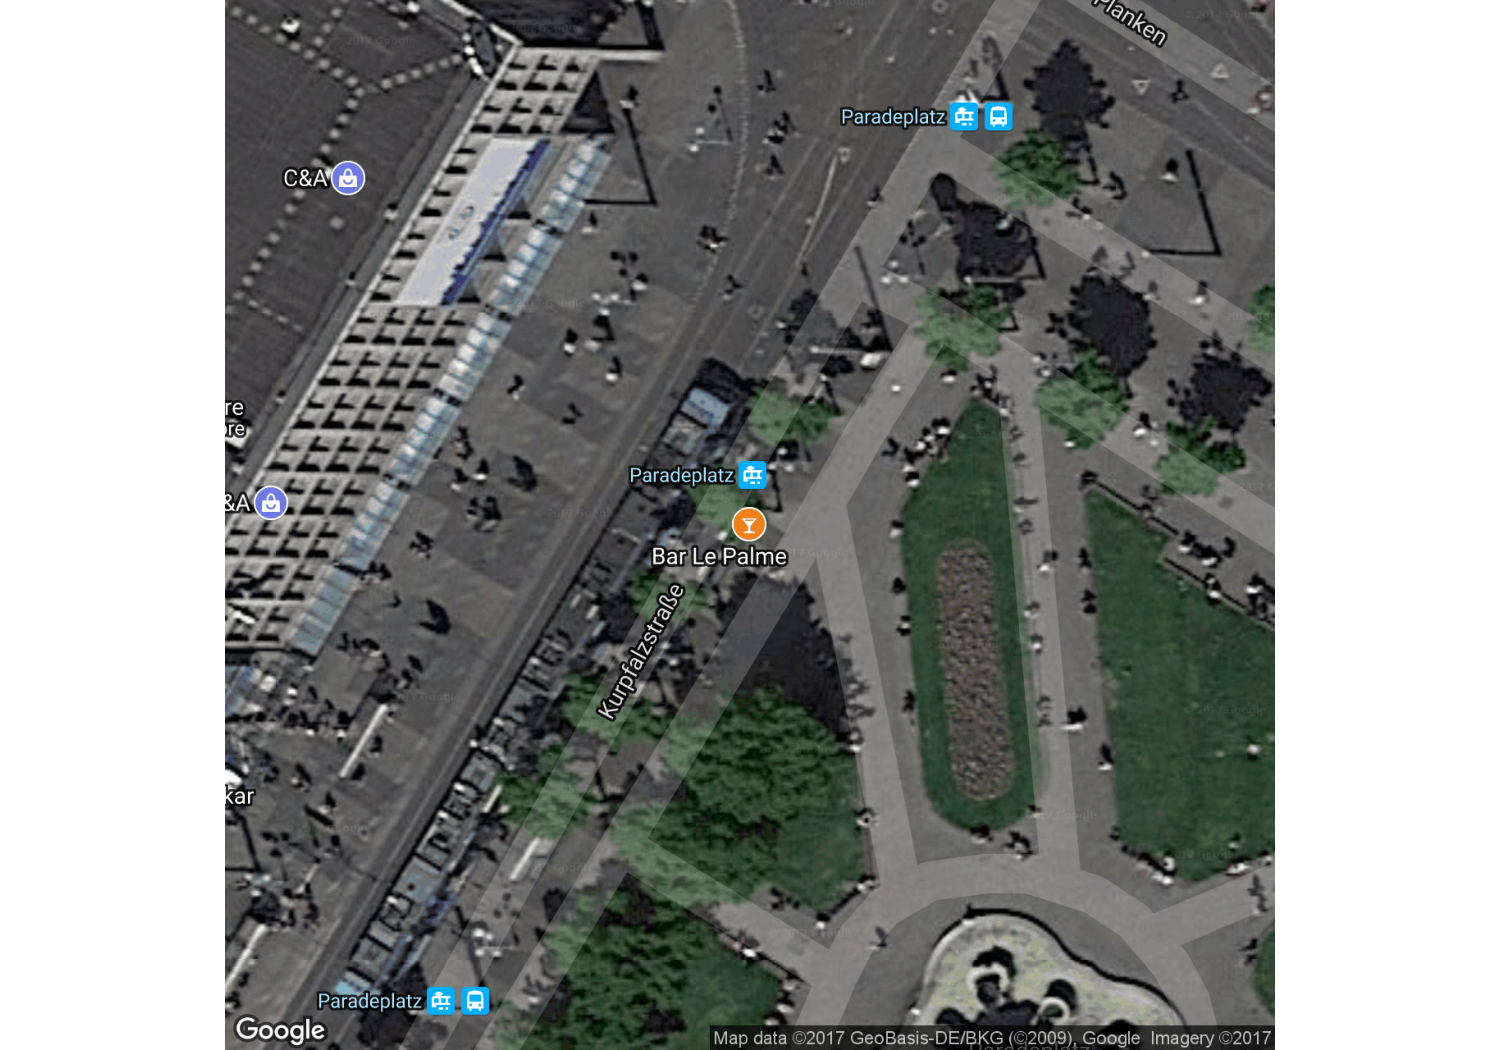
\includegraphics{RSocialScience2_files/figure-beamer/unnamed-chunk-38-1.pdf}
\caption{}
\end{figure}

\end{frame}

\begin{frame}[fragile]{ggmap - maptype hybrid}

\begin{Shaded}
\begin{Highlighting}[]
\KeywordTok{qmap}\NormalTok{(}\StringTok{"Mannheim"}\NormalTok{, }\DataTypeTok{zoom =} \DecValTok{14}\NormalTok{, }\DataTypeTok{maptype=}\StringTok{"hybrid"}\NormalTok{)}
\end{Highlighting}
\end{Shaded}

\begin{figure}[htbp]
\centering
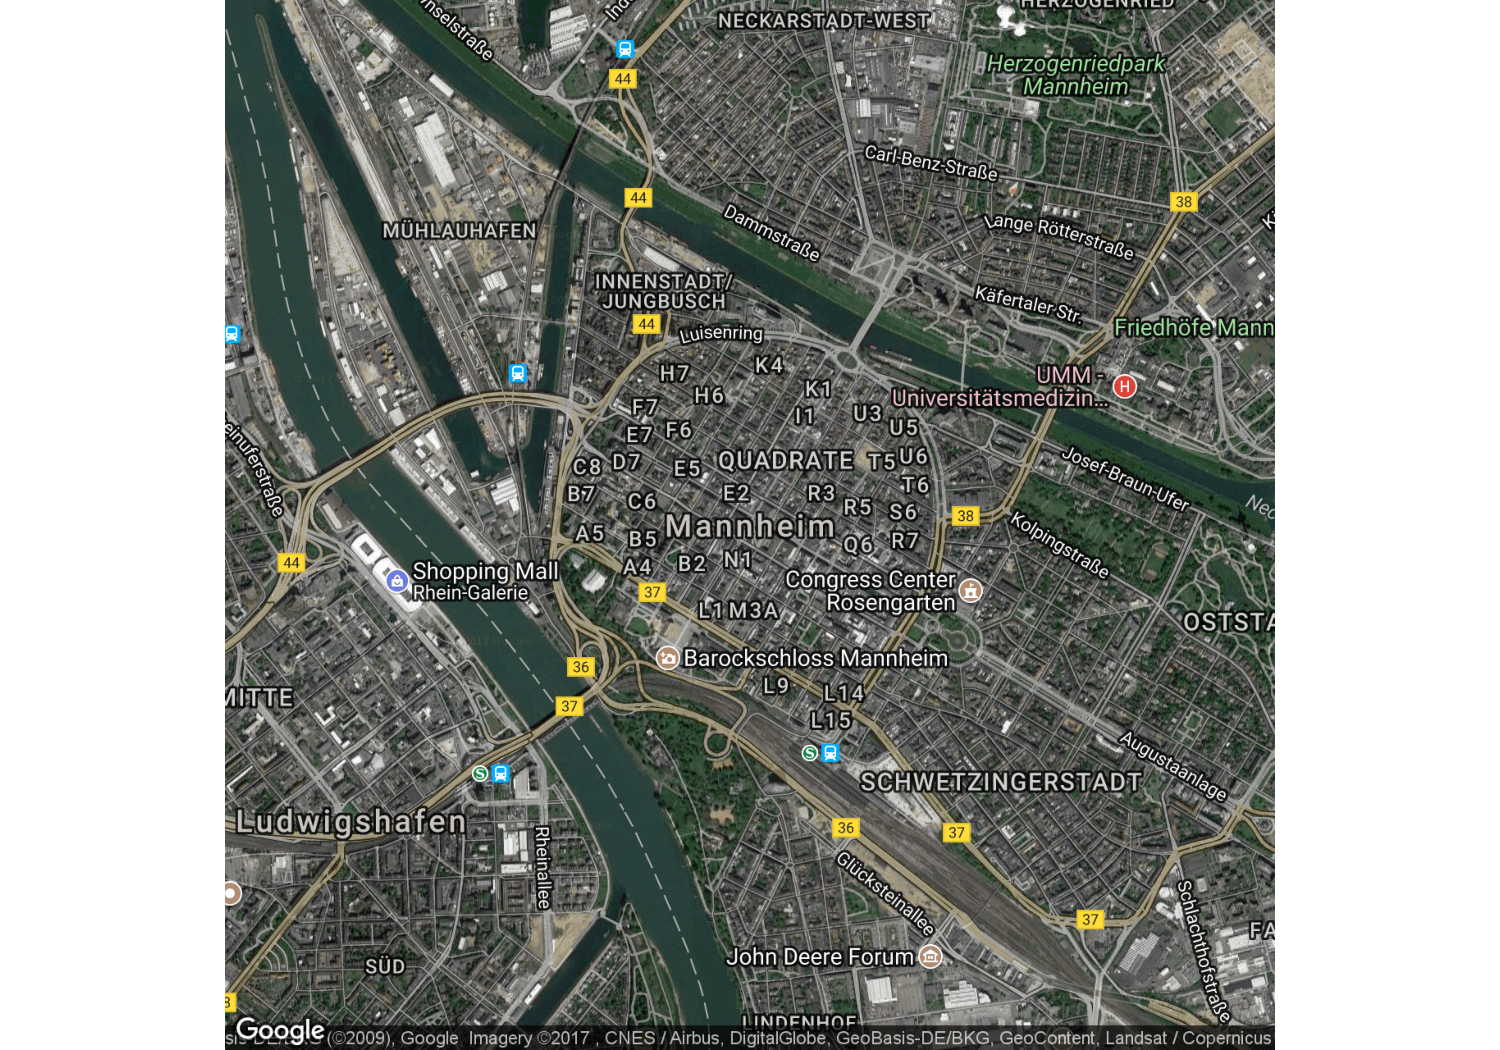
\includegraphics{RSocialScience2_files/figure-beamer/unnamed-chunk-39-1.pdf}
\caption{}
\end{figure}

\end{frame}

\begin{frame}{Terrain/physical maps}

\begin{itemize}
\item
  Aus Physischen Karten kann man Informationen über Berge, Flüsse und
  Seen ablesen.
\item
  Farben werden oft genutzt um Höhenunterschiede zu visualisieren
\end{itemize}

\end{frame}

\begin{frame}[fragile]{ggmap - terrain map}

\begin{Shaded}
\begin{Highlighting}[]
\KeywordTok{qmap}\NormalTok{(}\StringTok{'Schriesheim'}\NormalTok{, }\DataTypeTok{zoom =} \DecValTok{14}\NormalTok{,}\DataTypeTok{maptype=}\StringTok{"terrain"}\NormalTok{)}
\end{Highlighting}
\end{Shaded}

\begin{figure}[htbp]
\centering
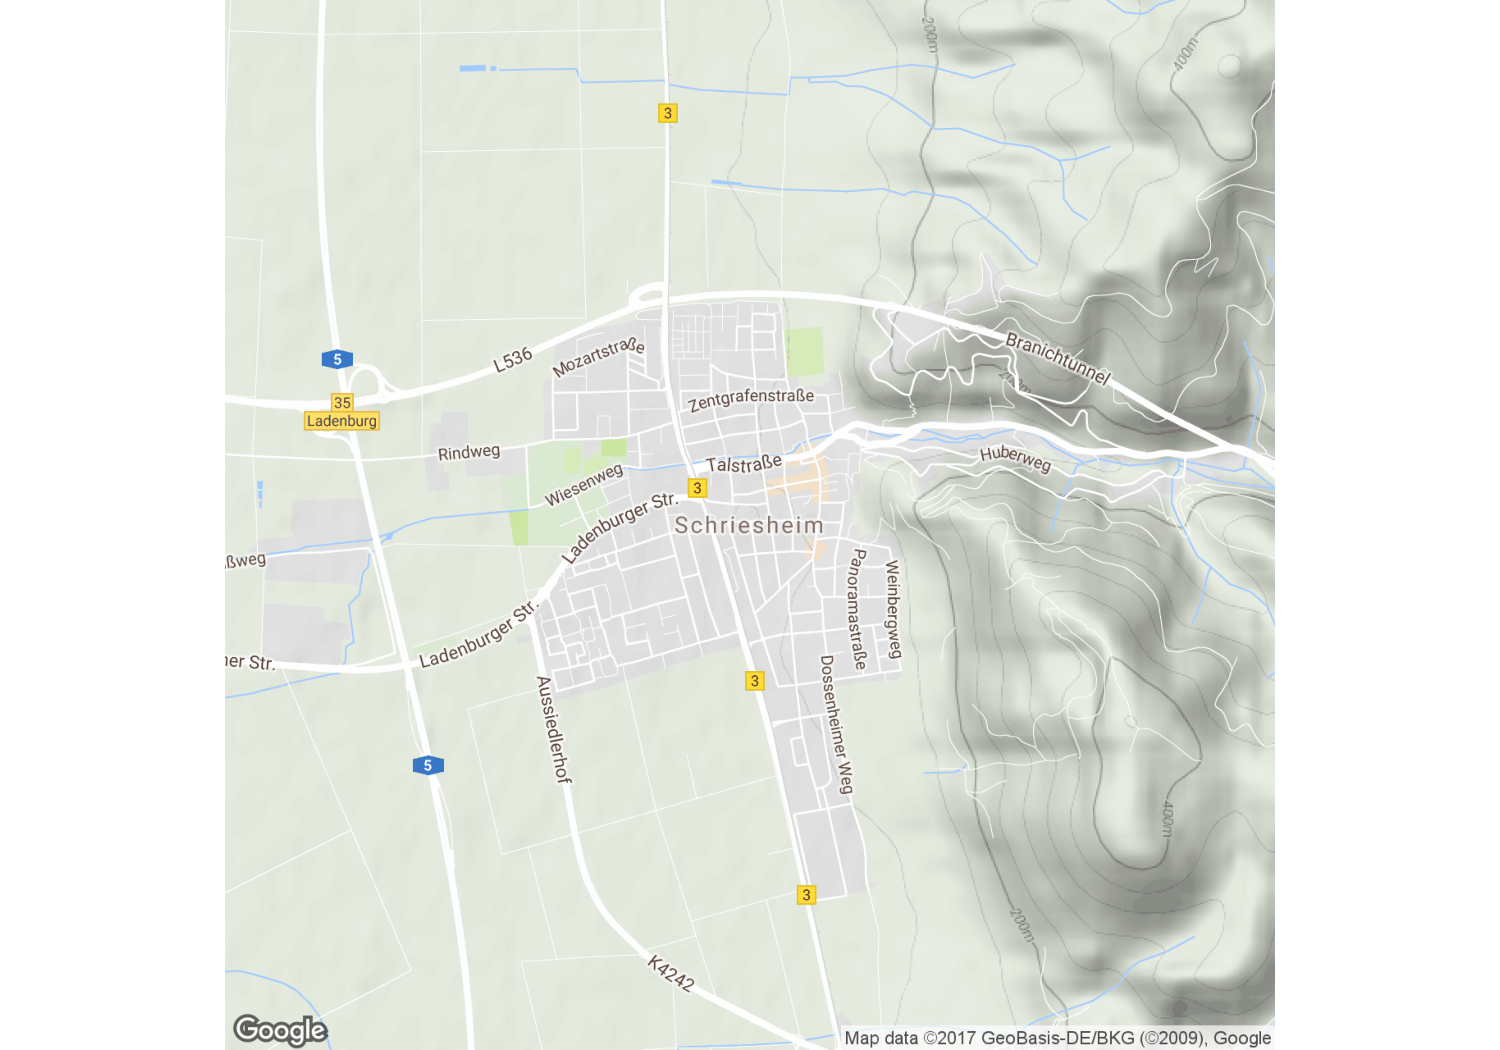
\includegraphics{RSocialScience2_files/figure-beamer/unnamed-chunk-40-1.pdf}
\caption{}
\end{figure}

\end{frame}

\begin{frame}{\href{http://www.designfaves.com/2014/03/abstracted-maps-reveal-cities-personalities}{Abstrahierte
Karten})}

\begin{figure}[htbp]
\centering
\includegraphics{https://github.com/Japhilko/IntroR/raw/master/2017/slides/figure/NYabstracted.jpg}
\caption{New York}
\end{figure}

\begin{itemize}
\tightlist
\item
  Abstraktion wird genutzt um nur essentielle Informationen zu zeigen.
\item
  Bsp. U-Bahn Karten - wichtig sind Richtungen und wenig Infos zur
  Orientierung
\item
  Nun kommen Karten, die sich als Hintergrund eignen.
\end{itemize}

\end{frame}

\begin{frame}[fragile]{ggmap - maptype watercolor}

\begin{Shaded}
\begin{Highlighting}[]
\KeywordTok{qmap}\NormalTok{(}\StringTok{'Mannheim'}\NormalTok{, }\DataTypeTok{zoom =} \DecValTok{14}\NormalTok{,}\DataTypeTok{maptype=}\StringTok{"watercolor"}\NormalTok{,}\DataTypeTok{source=}\StringTok{"stamen"}\NormalTok{)}
\end{Highlighting}
\end{Shaded}

\begin{figure}[htbp]
\centering
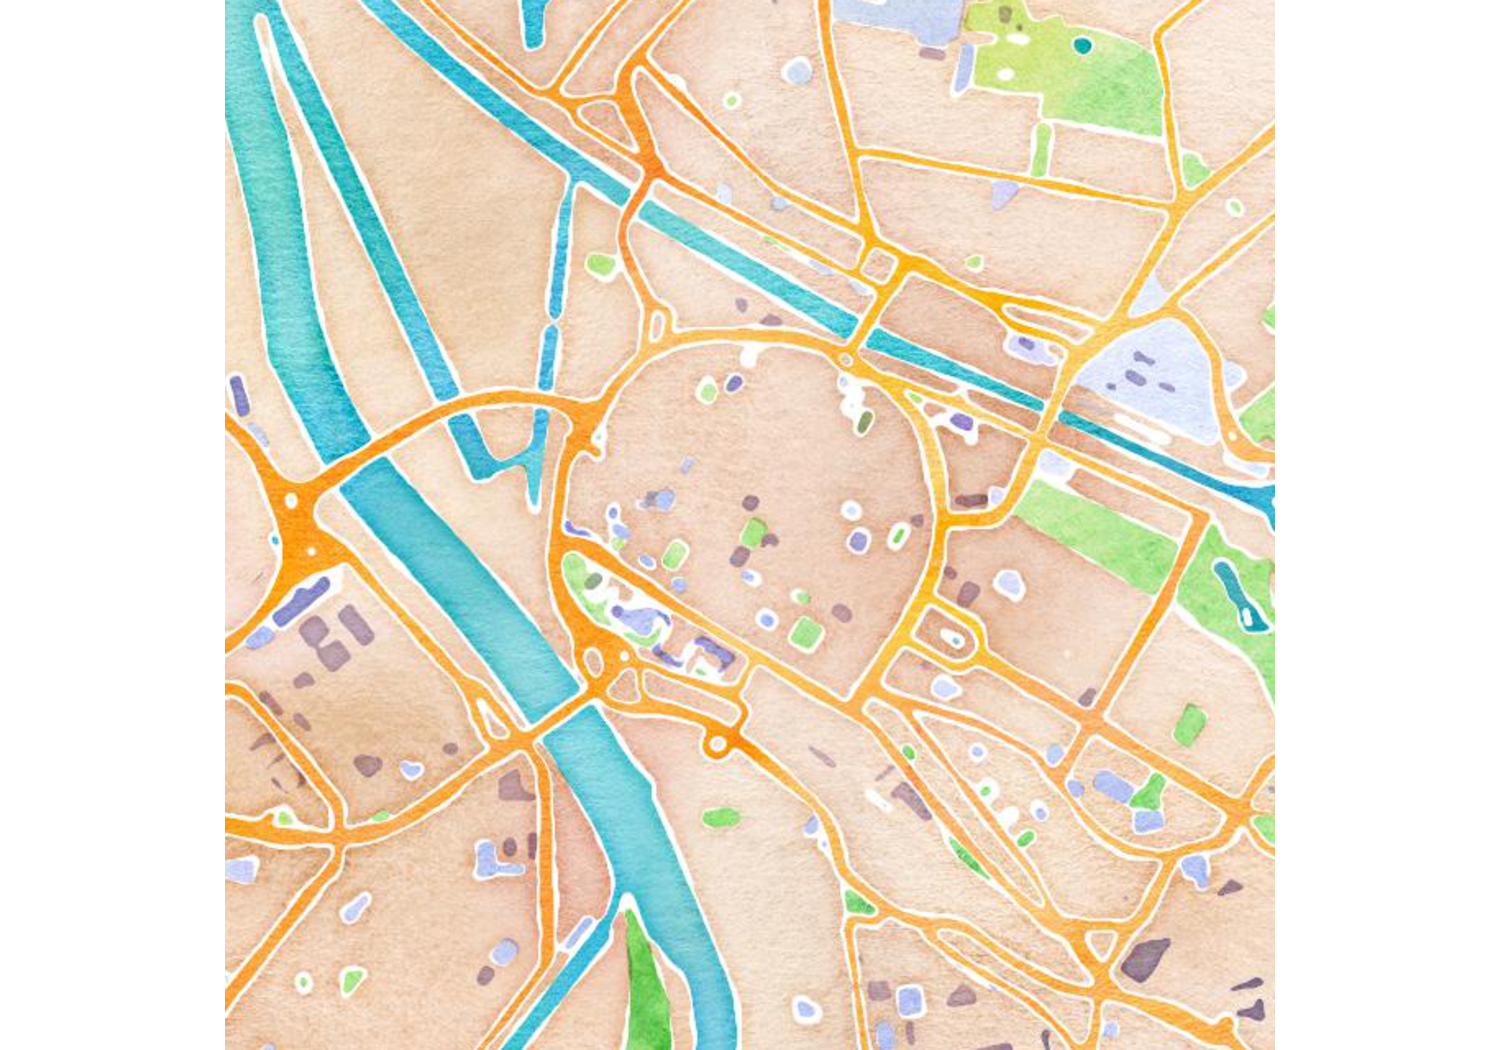
\includegraphics{RSocialScience2_files/figure-beamer/unnamed-chunk-41-1.pdf}
\caption{}
\end{figure}

\end{frame}

\begin{frame}[fragile]{ggmap - source stamen}

\begin{Shaded}
\begin{Highlighting}[]
\KeywordTok{qmap}\NormalTok{(}\StringTok{'Mannheim'}\NormalTok{, }\DataTypeTok{zoom =} \DecValTok{14}\NormalTok{,}
 \DataTypeTok{maptype=}\StringTok{"toner"}\NormalTok{,}\DataTypeTok{source=}\StringTok{"stamen"}\NormalTok{)}
\end{Highlighting}
\end{Shaded}

\begin{figure}[htbp]
\centering
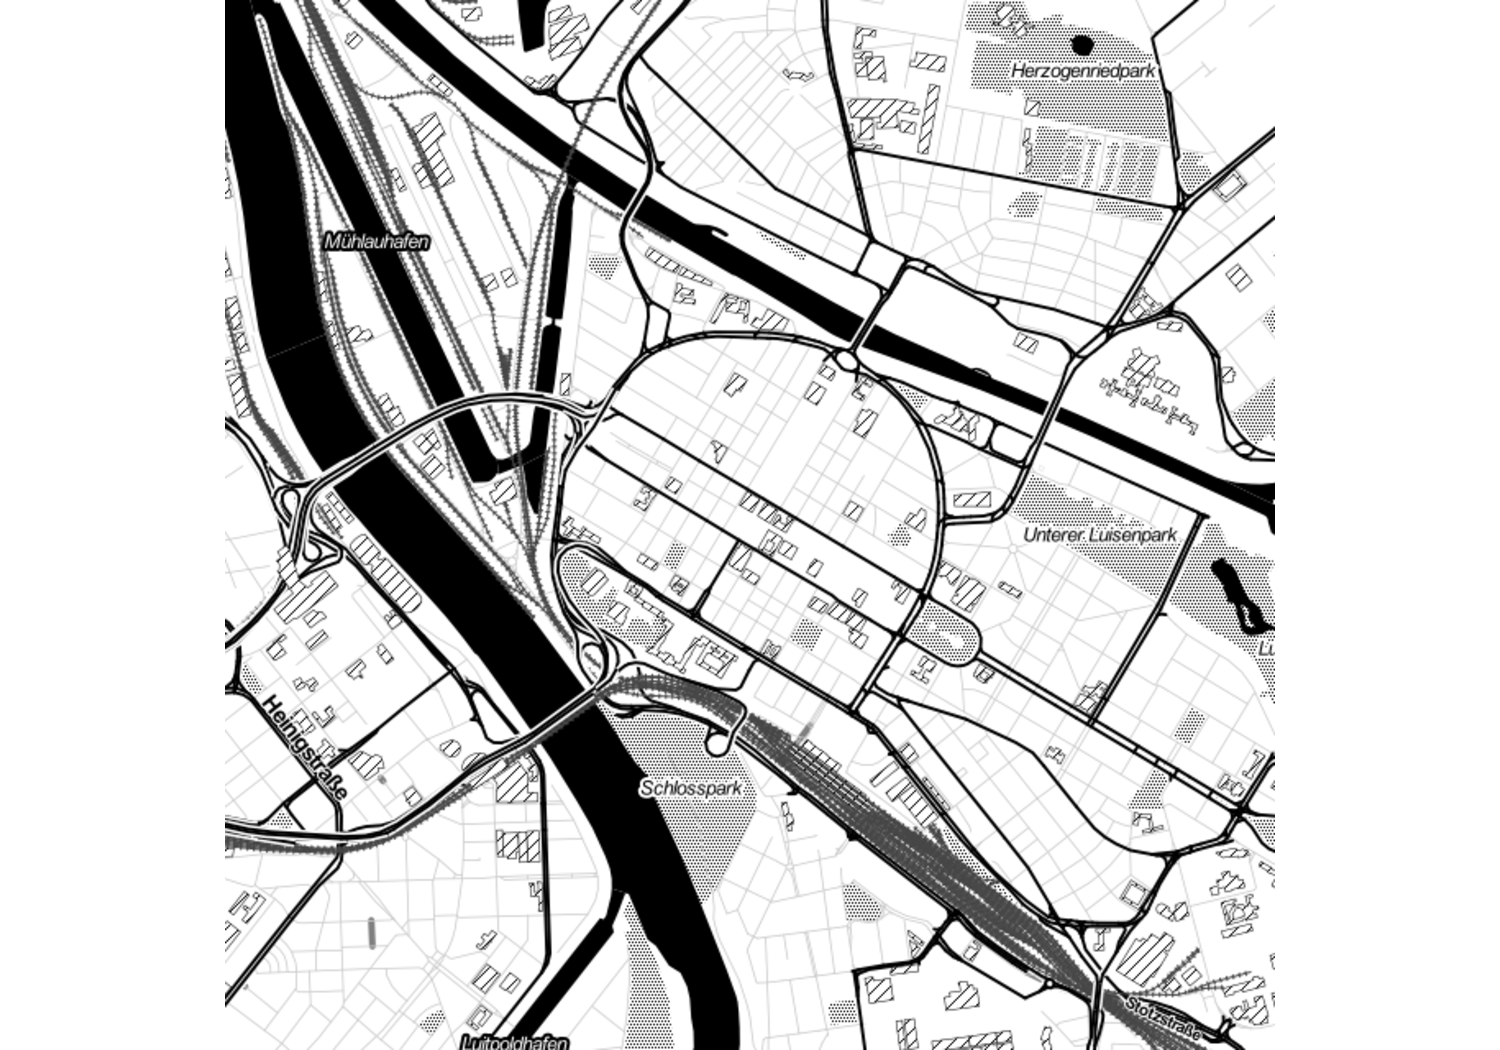
\includegraphics{RSocialScience2_files/figure-beamer/unnamed-chunk-42-1.pdf}
\caption{}
\end{figure}

\end{frame}

\begin{frame}[fragile]{ggmap - maptype toner-lite}

\begin{Shaded}
\begin{Highlighting}[]
\KeywordTok{qmap}\NormalTok{(}\StringTok{'Mannheim'}\NormalTok{, }\DataTypeTok{zoom =} \DecValTok{14}\NormalTok{,}
 \DataTypeTok{maptype=}\StringTok{"toner-lite"}\NormalTok{,}\DataTypeTok{source=}\StringTok{"stamen"}\NormalTok{)}
\end{Highlighting}
\end{Shaded}

\begin{figure}[htbp]
\centering
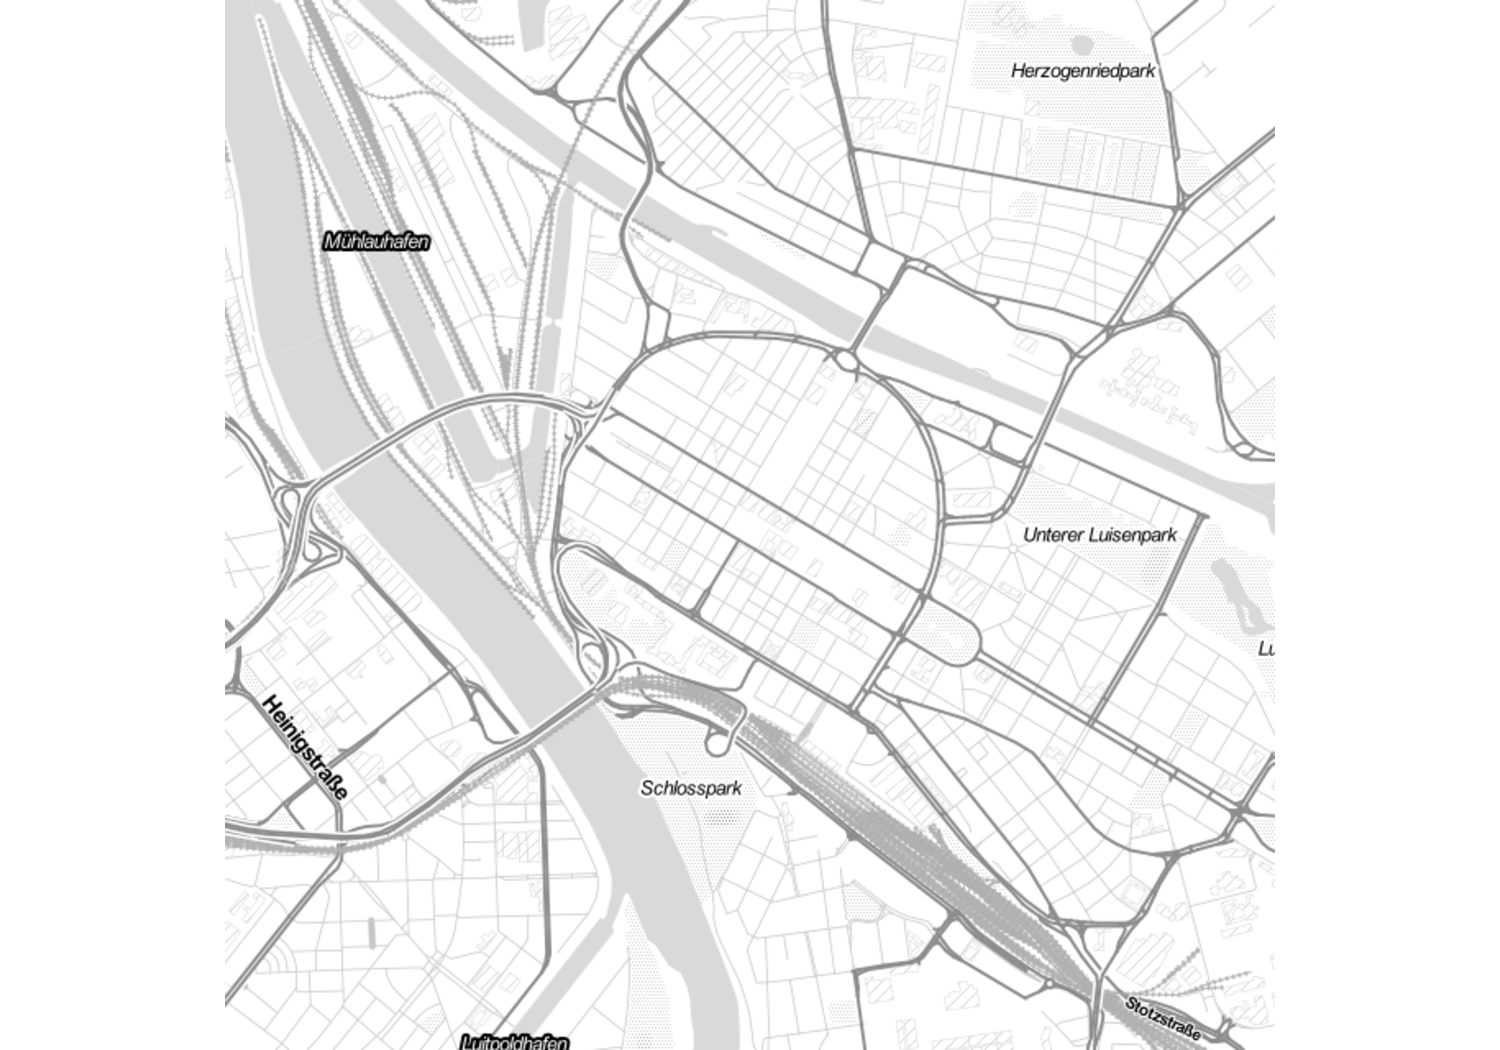
\includegraphics{RSocialScience2_files/figure-beamer/unnamed-chunk-43-1.pdf}
\caption{}
\end{figure}

\end{frame}

\begin{frame}[fragile]{ggmap - maptype toner-hybrid}

\begin{Shaded}
\begin{Highlighting}[]
\KeywordTok{qmap}\NormalTok{(}\StringTok{'Mannheim'}\NormalTok{, }\DataTypeTok{zoom =} \DecValTok{14}\NormalTok{,}
 \DataTypeTok{maptype=}\StringTok{"toner-hybrid"}\NormalTok{,}\DataTypeTok{source=}\StringTok{"stamen"}\NormalTok{)}
\end{Highlighting}
\end{Shaded}

\begin{figure}[htbp]
\centering
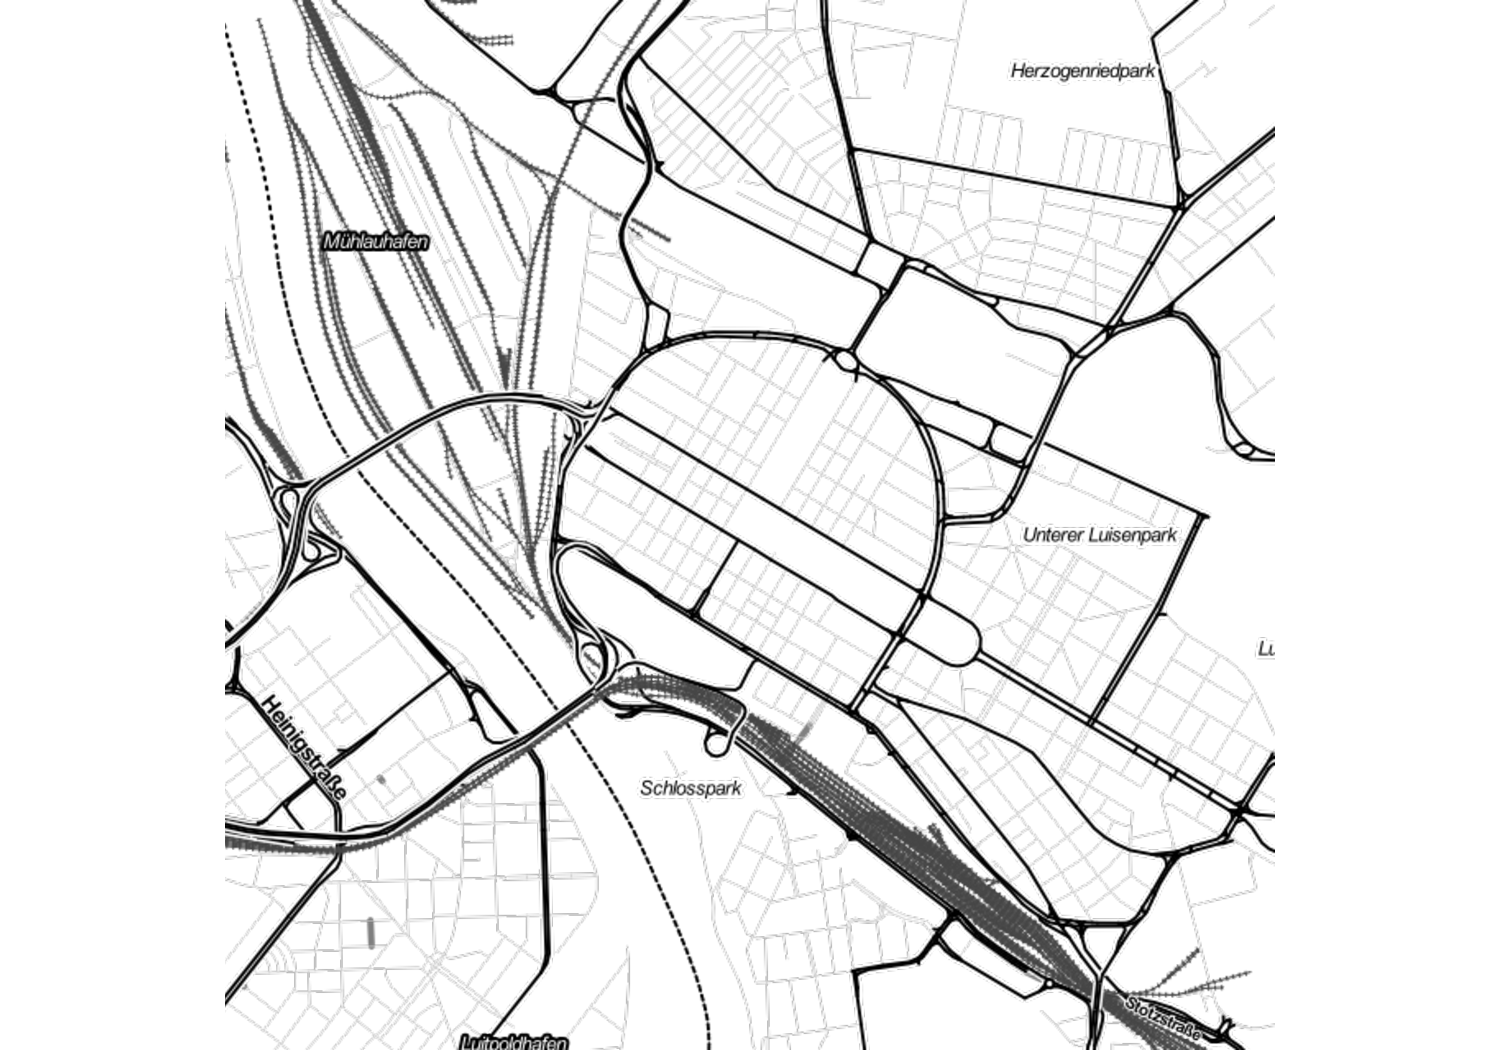
\includegraphics{RSocialScience2_files/figure-beamer/unnamed-chunk-44-1.pdf}
\caption{}
\end{figure}

\end{frame}

\begin{frame}[fragile]{ggmap - maptype terrain-lines}

\begin{Shaded}
\begin{Highlighting}[]
\KeywordTok{qmap}\NormalTok{(}\StringTok{'Mannheim'}\NormalTok{, }\DataTypeTok{zoom =} \DecValTok{14}\NormalTok{,}
 \DataTypeTok{maptype=}\StringTok{"terrain-lines"}\NormalTok{,}\DataTypeTok{source=}\StringTok{"stamen"}\NormalTok{)}
\end{Highlighting}
\end{Shaded}

\begin{figure}[htbp]
\centering
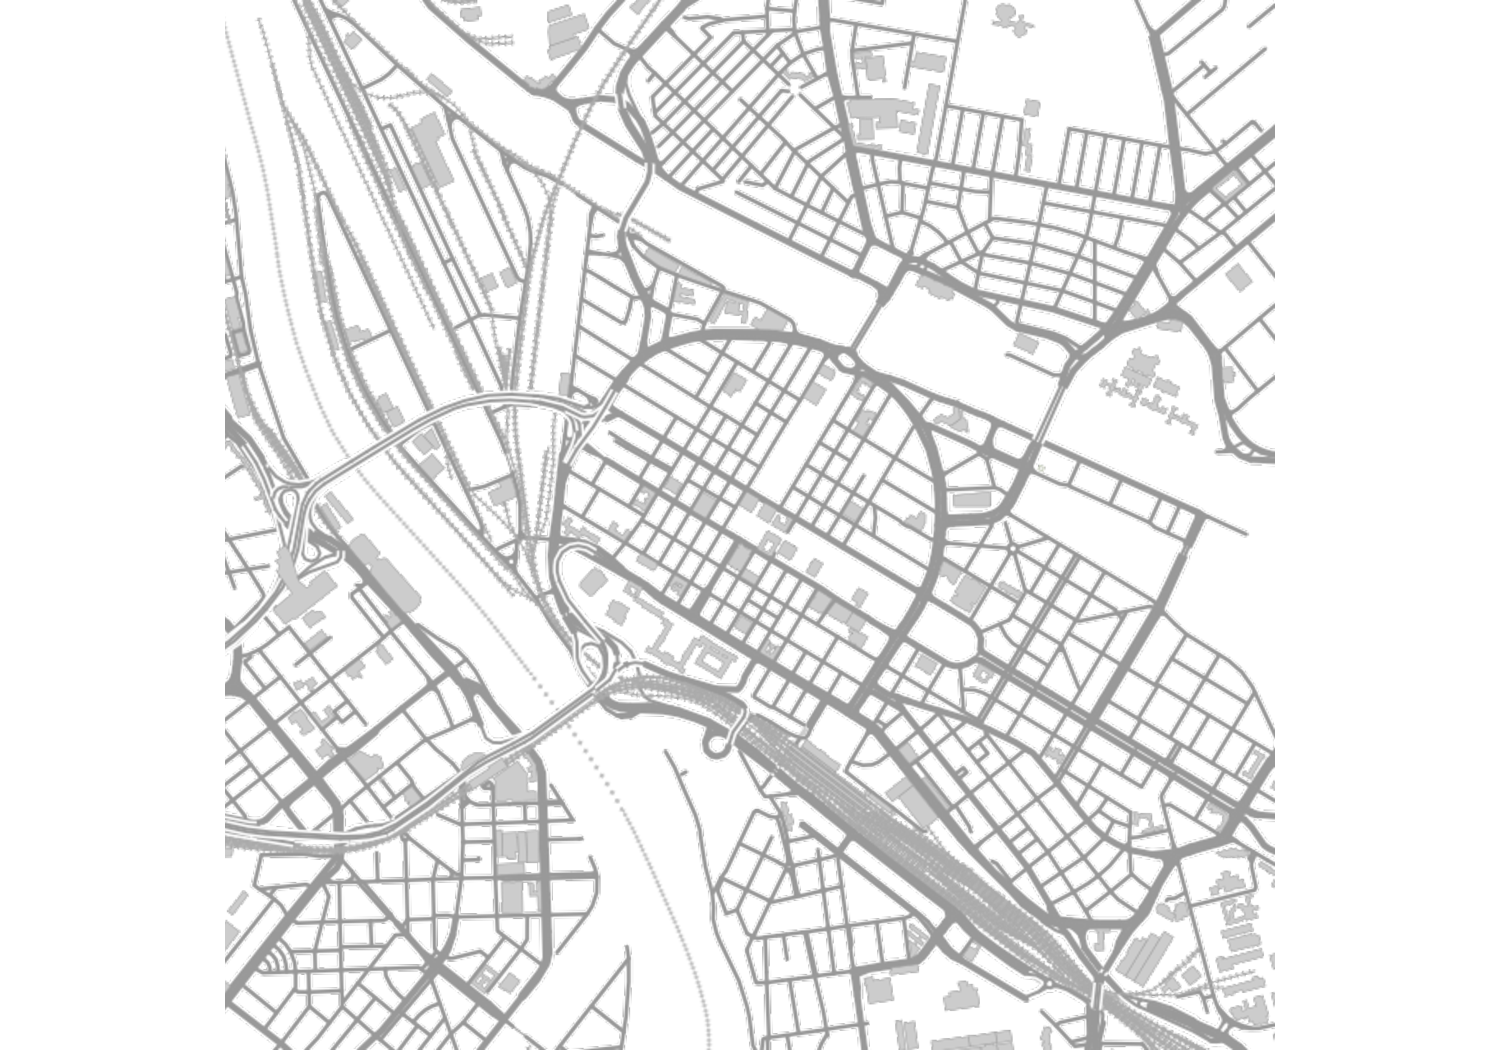
\includegraphics{RSocialScience2_files/figure-beamer/unnamed-chunk-45-1.pdf}
\caption{}
\end{figure}

\end{frame}

\begin{frame}{Graphiken speichern}

\begin{figure}[htbp]
\centering
\includegraphics{https://github.com/Japhilko/IntroR/raw/master/2017/slides/figure/RstudioExport.PNG}
\caption{RstudioExport}
\end{figure}

\end{frame}

\begin{frame}[fragile]{ggmap - ein Objekt erzeugen}

\begin{itemize}
\tightlist
\item
  \texttt{\textless{}-} ist der Zuweisungspfeil um ein Objekt zu
  erzeugen
\item
  Dieses Vorgehen macht bspw. Sinn, wenn mehrere Karten nebeneinander
  gebraucht werden.
\end{itemize}

\begin{Shaded}
\begin{Highlighting}[]
\NormalTok{MA_map <-}\StringTok{ }\KeywordTok{qmap}\NormalTok{(}\StringTok{'Mannheim'}\NormalTok{, }
               \DataTypeTok{zoom =} \DecValTok{14}\NormalTok{,}
               \DataTypeTok{maptype=}\StringTok{"toner"}\NormalTok{,}
               \DataTypeTok{source=}\StringTok{"stamen"}\NormalTok{)}
\end{Highlighting}
\end{Shaded}

\end{frame}

\begin{frame}[fragile]{Geokodierung}

\begin{quote}
Geocoding (\ldots{}) uses a description of a location, most typically a
postal address or place name, to find geographic coordinates from
spatial reference data \ldots{}
\end{quote}

\href{https://github.com/adam-p/markdown-here/wiki/Markdown-Cheatsheet\#blockquotes}{Wikipedia
- Geocoding}

\begin{Shaded}
\begin{Highlighting}[]
\KeywordTok{library}\NormalTok{(ggmap)}
\KeywordTok{geocode}\NormalTok{(}\StringTok{"Mannheim"}\NormalTok{,}\DataTypeTok{source=}\StringTok{"google"}\NormalTok{)}
\end{Highlighting}
\end{Shaded}

\begin{longtable}[]{@{}rr@{}}
\toprule
lon & lat\tabularnewline
\midrule
\endhead
8.463182 & 49.48608\tabularnewline
\bottomrule
\end{longtable}

\end{frame}

\begin{frame}{Latitude und Longitude}

\begin{figure}[htbp]
\centering
\includegraphics{https://github.com/Japhilko/IntroR/raw/master/2017/slides/figure/definition-of-latitude-longitude.jpg}
\caption{LatLon}
\end{figure}

\href{http://modernsurvivalblog.com/survival-skills/basic-map-reading-latitude-longitude/}{http://modernsurvivalblog.com}

\end{frame}

\begin{frame}{Koordinaten verschiedener Orte in Deutschland}

\begin{longtable}[]{@{}lrr@{}}
\toprule
cities & lon & lat\tabularnewline
\midrule
\endhead
Hamburg & 9.993682 & 53.55108\tabularnewline
Koeln & 6.960279 & 50.93753\tabularnewline
Dresden & 13.737262 & 51.05041\tabularnewline
Muenchen & 11.581981 & 48.13513\tabularnewline
\bottomrule
\end{longtable}

\end{frame}

\begin{frame}[fragile]{Reverse Geokodierung}

\begin{quote}
Reverse geocoding is the process of back (reverse) coding of a point
location (latitude, longitude) to a readable address or place name. This
permits the identification of nearby street addresses, places, and/or
areal subdivisions such as neighbourhoods, county, state, or country.
\end{quote}

Quelle:
\href{https://en.wikipedia.org/wiki/Reverse_geocoding}{Wikipedia}

\begin{Shaded}
\begin{Highlighting}[]
\KeywordTok{revgeocode}\NormalTok{(}\KeywordTok{c}\NormalTok{(}\DecValTok{48}\NormalTok{,}\DecValTok{8}\NormalTok{))}
\end{Highlighting}
\end{Shaded}

\begin{verbatim}
## [1] "Unnamed Road, Somalia"
\end{verbatim}

\end{frame}

\begin{frame}[fragile]{Die Distanz zwischen zwei Punkten}

\begin{Shaded}
\begin{Highlighting}[]
\KeywordTok{mapdist}\NormalTok{(}\StringTok{"Q1, 4 Mannheim"}\NormalTok{,}\StringTok{"B2, 1 Mannheim"}\NormalTok{)}
\end{Highlighting}
\end{Shaded}

\begin{verbatim}
##             from             to   m    km     miles seconds  minutes
## 1 Q1, 4 Mannheim B2, 1 Mannheim 749 0.749 0.4654286     215 3.583333
##        hours
## 1 0.05972222
\end{verbatim}

\begin{Shaded}
\begin{Highlighting}[]
\KeywordTok{mapdist}\NormalTok{(}\StringTok{"Q1, 4 Mannheim"}\NormalTok{,}\StringTok{"B2, 1 Mannheim"}\NormalTok{,}\DataTypeTok{mode=}\StringTok{"walking"}\NormalTok{)}
\end{Highlighting}
\end{Shaded}

\begin{verbatim}
##             from             to   m    km     miles seconds minutes  hours
## 1 Q1, 4 Mannheim B2, 1 Mannheim 546 0.546 0.3392844     423    7.05 0.1175
\end{verbatim}

\end{frame}

\begin{frame}[fragile]{Eine andere Distanz bekommen}

\begin{Shaded}
\begin{Highlighting}[]
\KeywordTok{mapdist}\NormalTok{(}\StringTok{"Q1, 4 Mannheim"}\NormalTok{,}\StringTok{"B2, 1 Mannheim"}\NormalTok{,}\DataTypeTok{mode=}\StringTok{"bicycling"}\NormalTok{)}
\end{Highlighting}
\end{Shaded}

\begin{verbatim}
##             from             to   m    km    miles seconds  minutes
## 1 Q1, 4 Mannheim B2, 1 Mannheim 555 0.555 0.344877     215 3.583333
##        hours
## 1 0.05972222
\end{verbatim}

\end{frame}

\begin{frame}[fragile]{Geokodierung - verschiedene Punkte von Interesse}

\begin{Shaded}
\begin{Highlighting}[]
\NormalTok{POI1 <-}\StringTok{ }\KeywordTok{geocode}\NormalTok{(}\StringTok{"B2, 1 Mannheim"}\NormalTok{,}\DataTypeTok{source=}\StringTok{"google"}\NormalTok{)}
\NormalTok{POI2 <-}\StringTok{ }\KeywordTok{geocode}\NormalTok{(}\StringTok{"Hbf Mannheim"}\NormalTok{,}\DataTypeTok{source=}\StringTok{"google"}\NormalTok{)}
\NormalTok{POI3 <-}\StringTok{ }\KeywordTok{geocode}\NormalTok{(}\StringTok{"Mannheim, Friedrichsplatz"}\NormalTok{,}\DataTypeTok{source=}\StringTok{"google"}\NormalTok{)}
\NormalTok{ListPOI <-}\KeywordTok{rbind}\NormalTok{(POI1,POI2,POI3)}
\NormalTok{POI1;POI2;POI3}
\end{Highlighting}
\end{Shaded}

\begin{verbatim}
##        lon      lat
## 1 8.462844 49.48569
\end{verbatim}

\begin{verbatim}
##        lon      lat
## 1 8.469879 49.47972
\end{verbatim}

\begin{verbatim}
##        lon      lat
## 1 8.475754 49.48304
\end{verbatim}

\end{frame}

\begin{frame}[fragile]{Punkte in der Karte}

\begin{Shaded}
\begin{Highlighting}[]
\NormalTok{MA_map +}
\KeywordTok{geom_point}\NormalTok{(}\KeywordTok{aes}\NormalTok{(}\DataTypeTok{x =} \NormalTok{lon, }\DataTypeTok{y =} \NormalTok{lat),}
\DataTypeTok{data =} \NormalTok{ListPOI)}
\end{Highlighting}
\end{Shaded}

\begin{figure}[htbp]
\centering
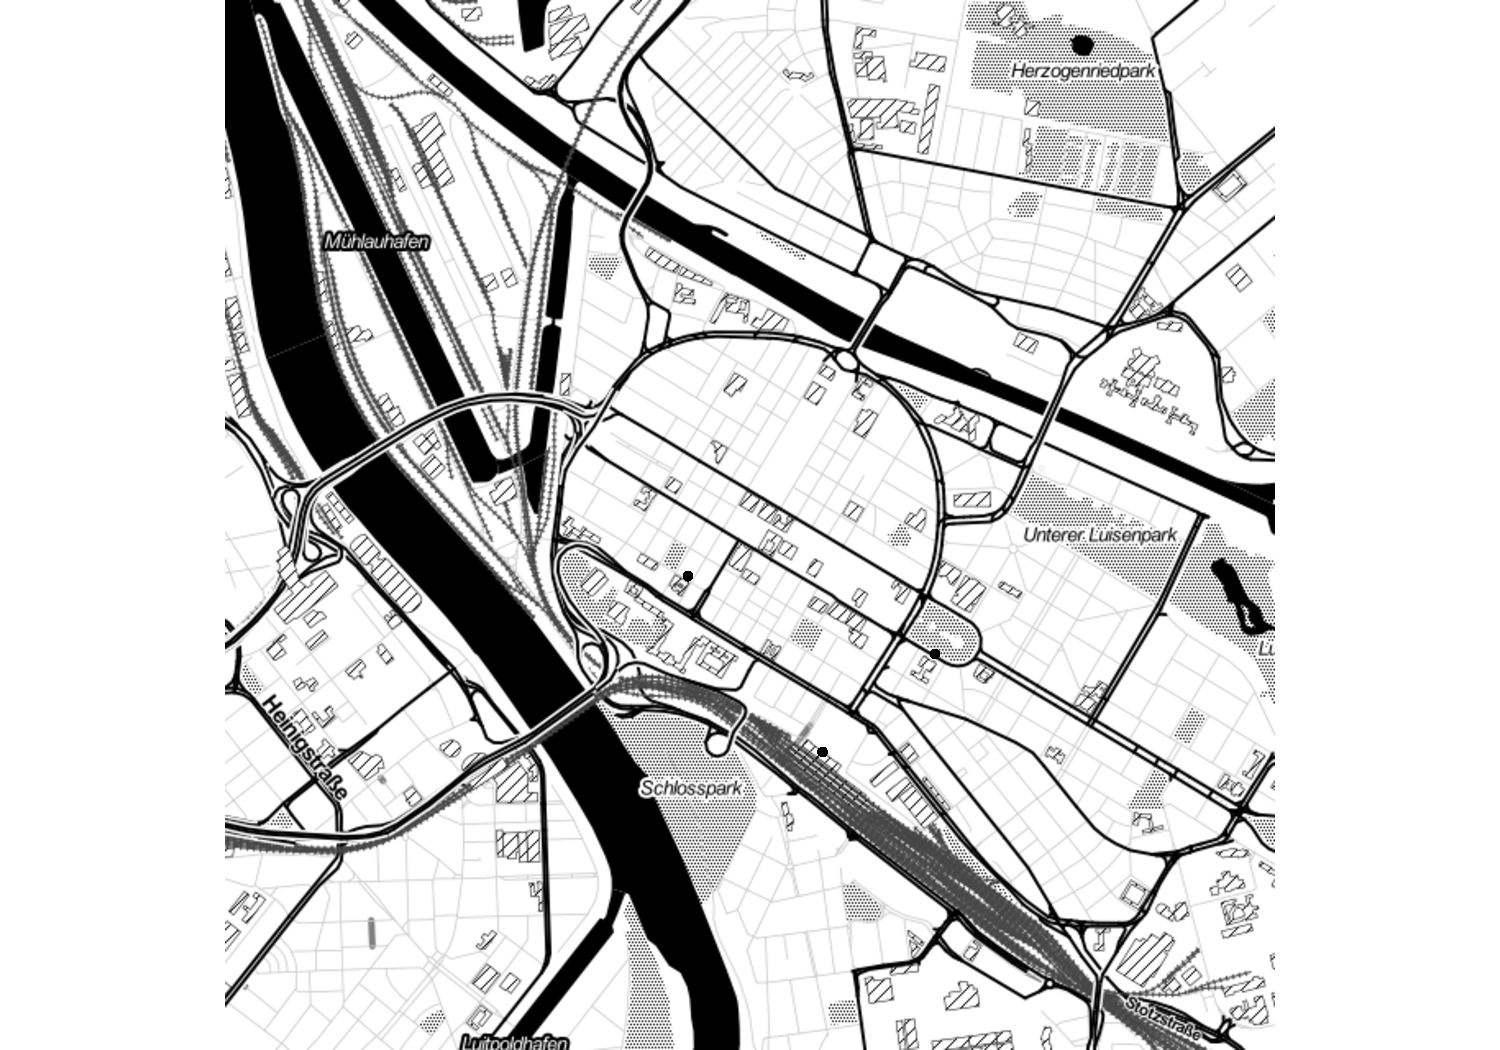
\includegraphics{RSocialScience2_files/figure-beamer/unnamed-chunk-55-1.pdf}
\caption{}
\end{figure}

\end{frame}

\begin{frame}[fragile]{Punkte in der Karte}

\begin{Shaded}
\begin{Highlighting}[]
\NormalTok{MA_map +}
\KeywordTok{geom_point}\NormalTok{(}\KeywordTok{aes}\NormalTok{(}\DataTypeTok{x =} \NormalTok{lon, }\DataTypeTok{y =} \NormalTok{lat),}\DataTypeTok{col=}\StringTok{"red"}\NormalTok{,}
\DataTypeTok{data =} \NormalTok{ListPOI)}
\end{Highlighting}
\end{Shaded}

\begin{figure}[htbp]
\centering
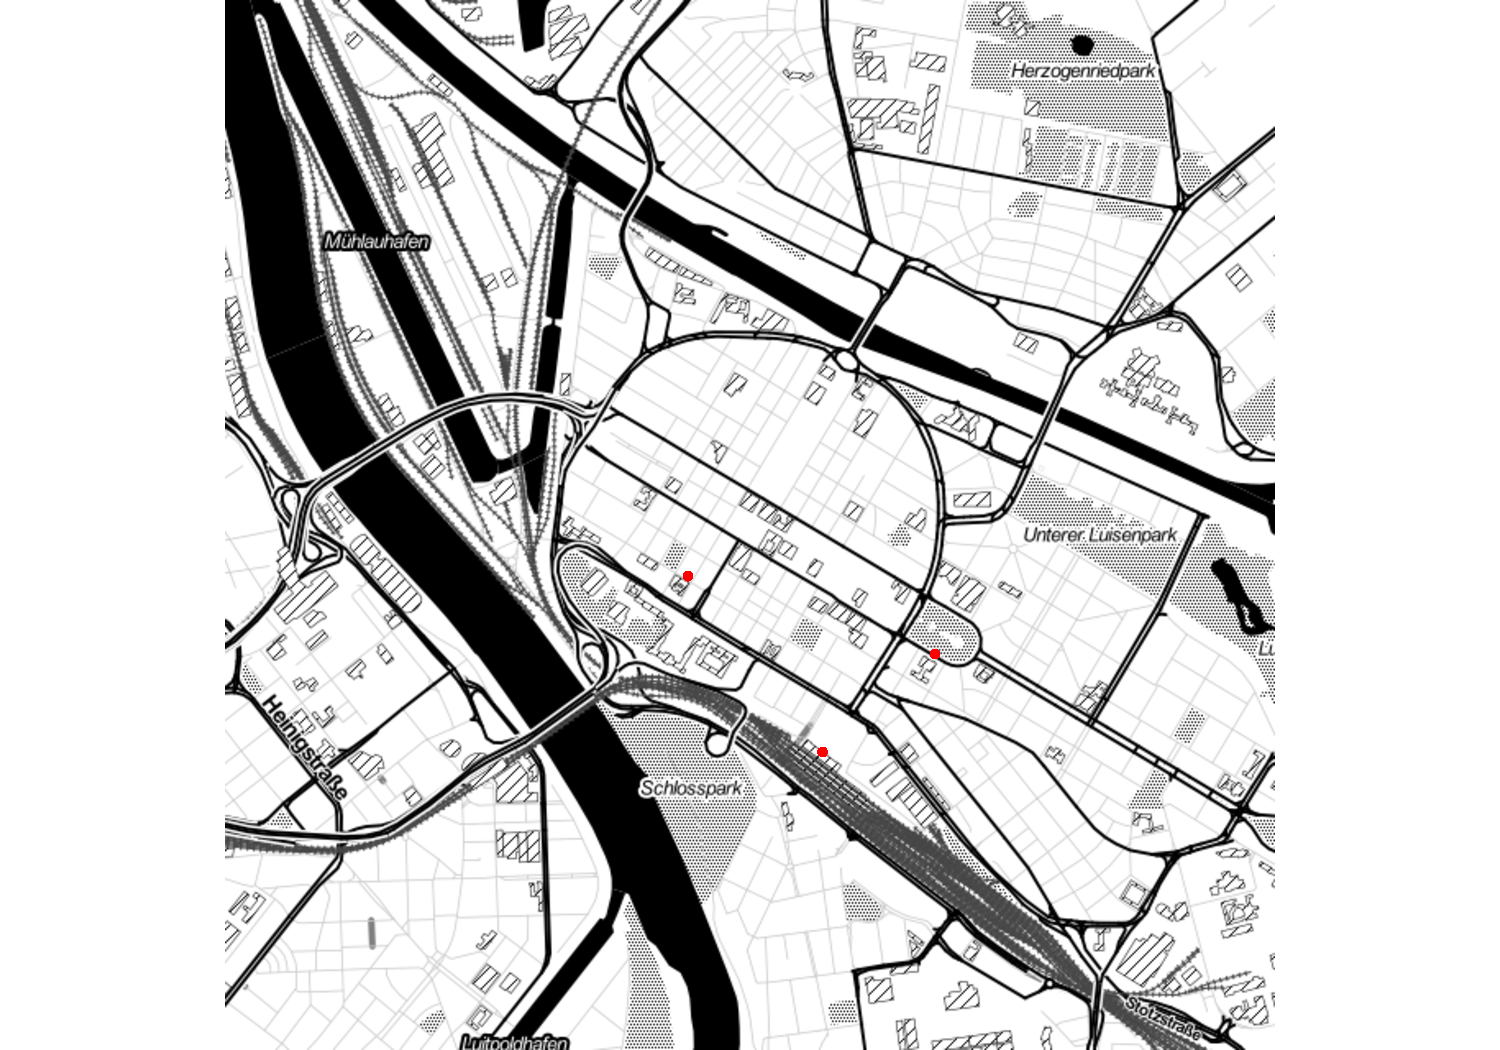
\includegraphics{RSocialScience2_files/figure-beamer/unnamed-chunk-56-1.pdf}
\caption{}
\end{figure}

\end{frame}

\begin{frame}[fragile]{ggmap - verschiedene Farben}

\begin{Shaded}
\begin{Highlighting}[]
\NormalTok{ListPOI$color <-}\StringTok{ }\KeywordTok{c}\NormalTok{(}\StringTok{"A"}\NormalTok{,}\StringTok{"B"}\NormalTok{,}\StringTok{"C"}\NormalTok{)}
\NormalTok{MA_map +}
\KeywordTok{geom_point}\NormalTok{(}\KeywordTok{aes}\NormalTok{(}\DataTypeTok{x =} \NormalTok{lon, }\DataTypeTok{y =} \NormalTok{lat,}\DataTypeTok{col=}\NormalTok{color),}
\DataTypeTok{data =} \NormalTok{ListPOI)}
\end{Highlighting}
\end{Shaded}

\begin{figure}[htbp]
\centering
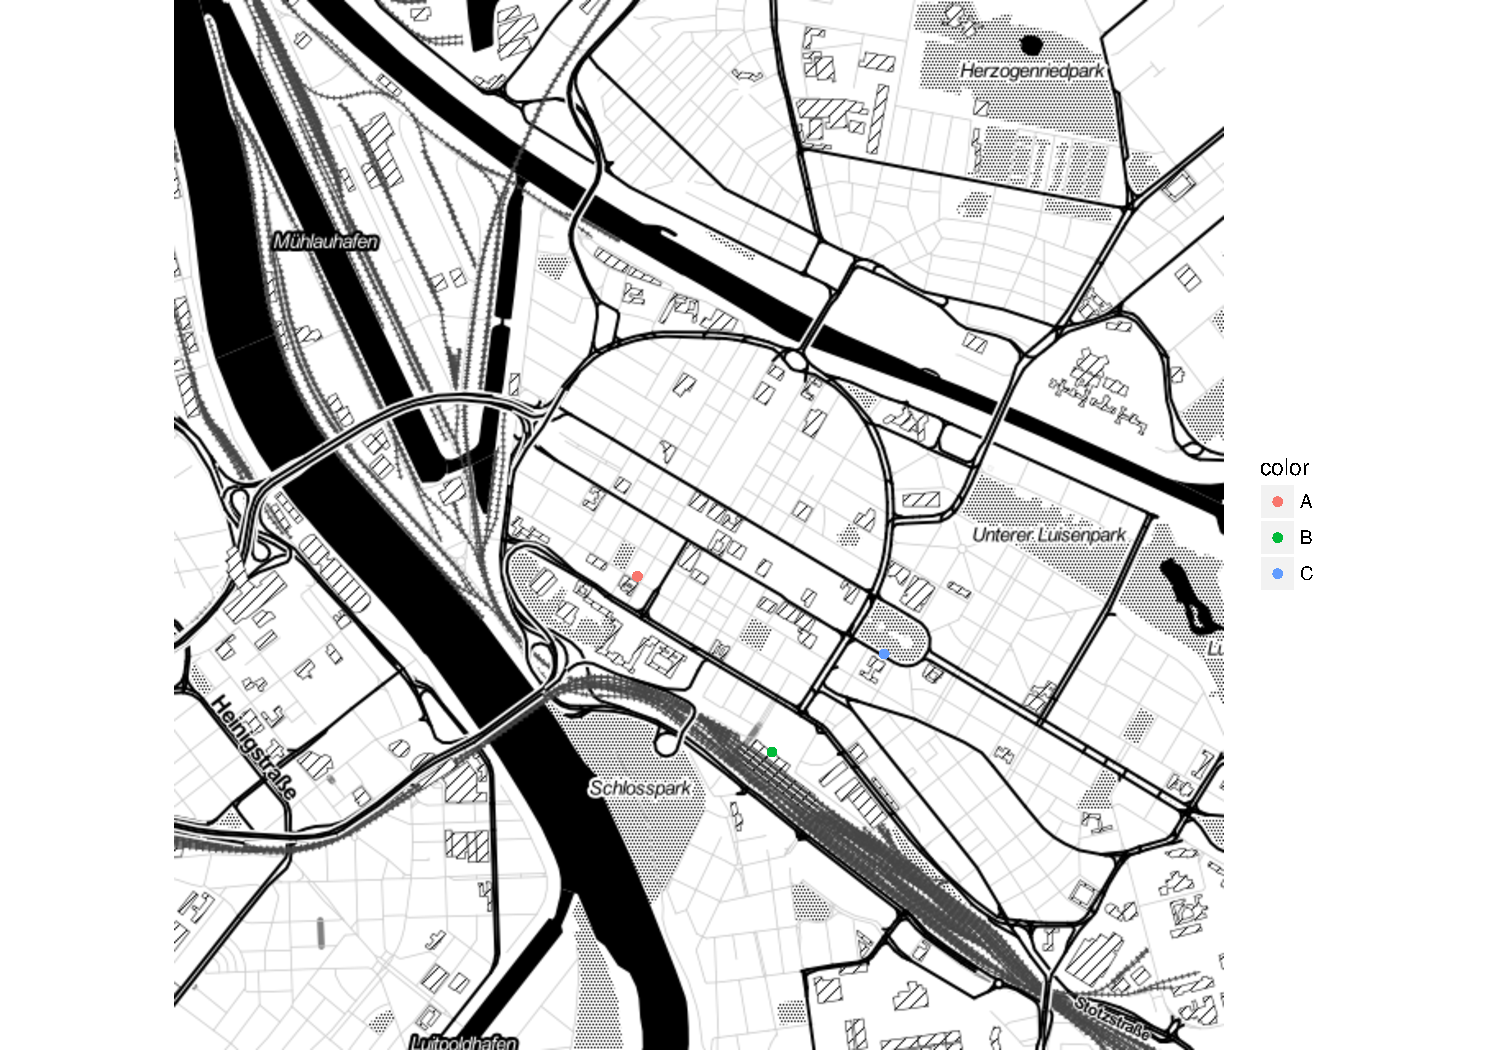
\includegraphics{RSocialScience2_files/figure-beamer/unnamed-chunk-57-1.pdf}
\caption{}
\end{figure}

\end{frame}

\begin{frame}[fragile]{ggmap - größere Punkte}

\begin{Shaded}
\begin{Highlighting}[]
\NormalTok{ListPOI$size <-}\StringTok{ }\KeywordTok{c}\NormalTok{(}\DecValTok{10}\NormalTok{,}\DecValTok{20}\NormalTok{,}\DecValTok{30}\NormalTok{)}
\NormalTok{MA_map +}
\KeywordTok{geom_point}\NormalTok{(}\KeywordTok{aes}\NormalTok{(}\DataTypeTok{x =} \NormalTok{lon, }\DataTypeTok{y =} \NormalTok{lat,}\DataTypeTok{col=}\NormalTok{color,}\DataTypeTok{size=}\NormalTok{size),}
\DataTypeTok{data =} \NormalTok{ListPOI)}
\end{Highlighting}
\end{Shaded}

\begin{figure}[htbp]
\centering
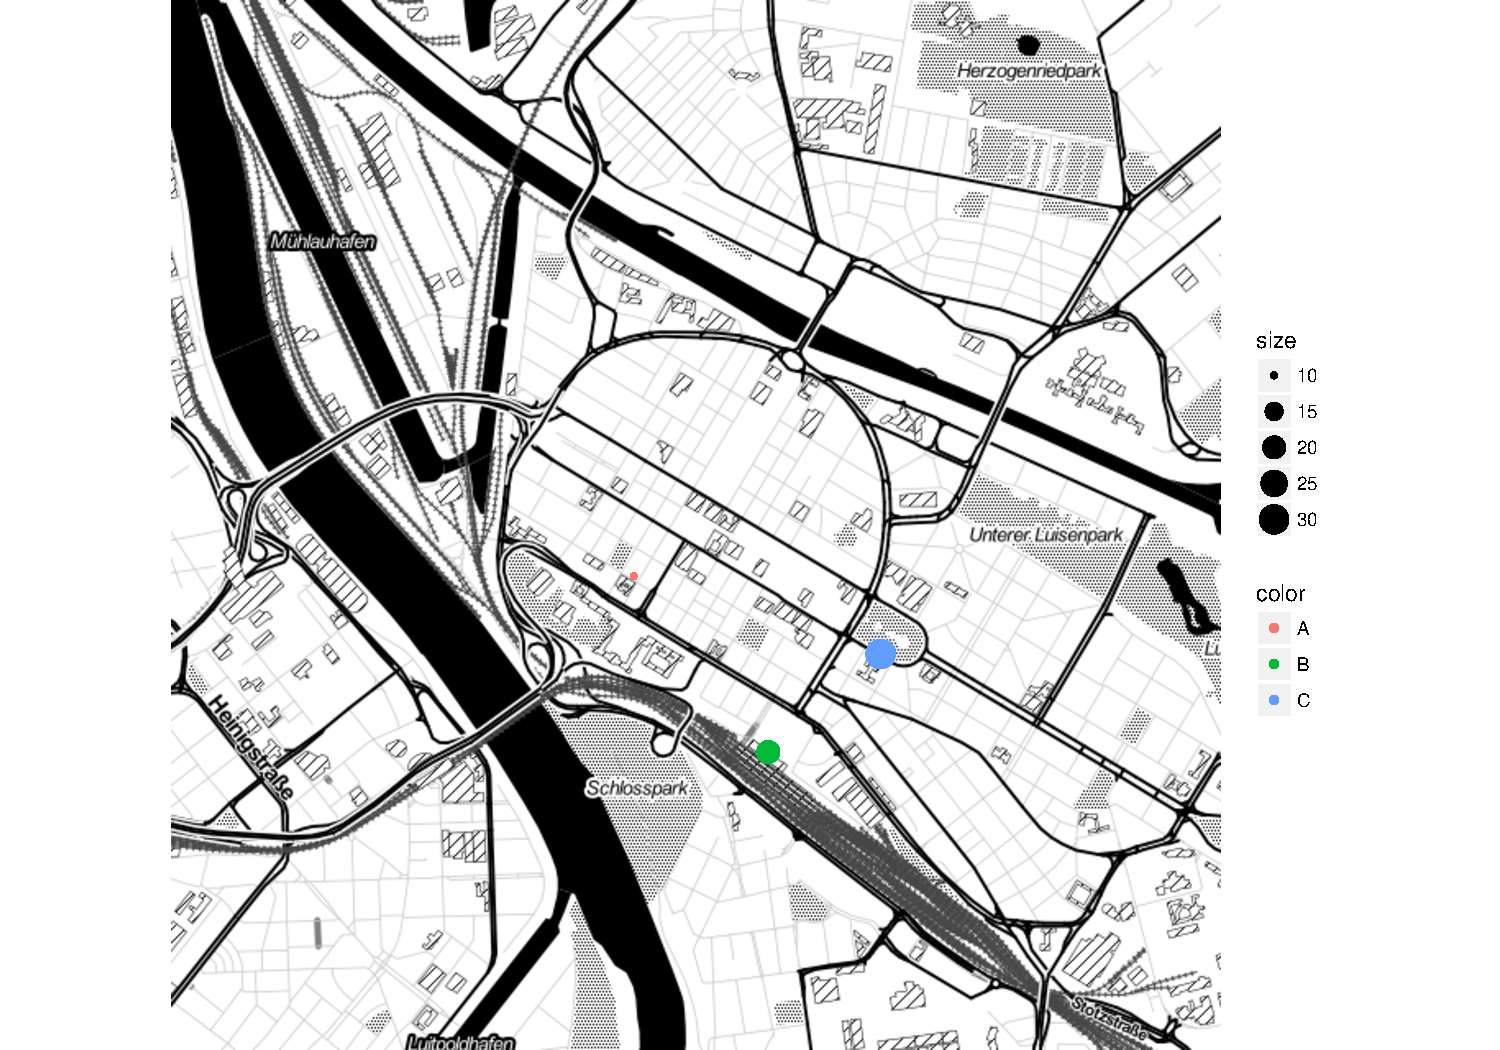
\includegraphics{RSocialScience2_files/figure-beamer/unnamed-chunk-58-1.pdf}
\caption{}
\end{figure}

\end{frame}

\begin{frame}[fragile]{Eine Route von Google maps bekommen}

\begin{Shaded}
\begin{Highlighting}[]
\NormalTok{from <-}\StringTok{ "Mannheim Hbf"}
\NormalTok{to <-}\StringTok{ "Mannheim B2 , 1"}
\NormalTok{route_df <-}\StringTok{ }\KeywordTok{route}\NormalTok{(from, to, }\DataTypeTok{structure =} \StringTok{"route"}\NormalTok{)}
\end{Highlighting}
\end{Shaded}

\href{http://rpackages.ianhowson.com/cran/ggmap/man/route.html}{Mehr
Information}

\url{http://rpackages.ianhowson.com/cran/ggmap/man/route.html}

\end{frame}

\begin{frame}[fragile]{Eine Karte mit dieser Information zeichnen}

\begin{Shaded}
\begin{Highlighting}[]
\KeywordTok{qmap}\NormalTok{(}\StringTok{"Mannheim Hbf"}\NormalTok{, }\DataTypeTok{zoom =} \DecValTok{14}\NormalTok{) +}
\StringTok{  }\KeywordTok{geom_path}\NormalTok{(}
    \KeywordTok{aes}\NormalTok{(}\DataTypeTok{x =} \NormalTok{lon, }\DataTypeTok{y =} \NormalTok{lat),  }\DataTypeTok{colour =} \StringTok{"red"}\NormalTok{, }\DataTypeTok{size =} \FloatTok{1.5}\NormalTok{,}
    \DataTypeTok{data =} \NormalTok{route_df, }\DataTypeTok{lineend =} \StringTok{"round"}
  \NormalTok{)}
\end{Highlighting}
\end{Shaded}

\begin{figure}[htbp]
\centering
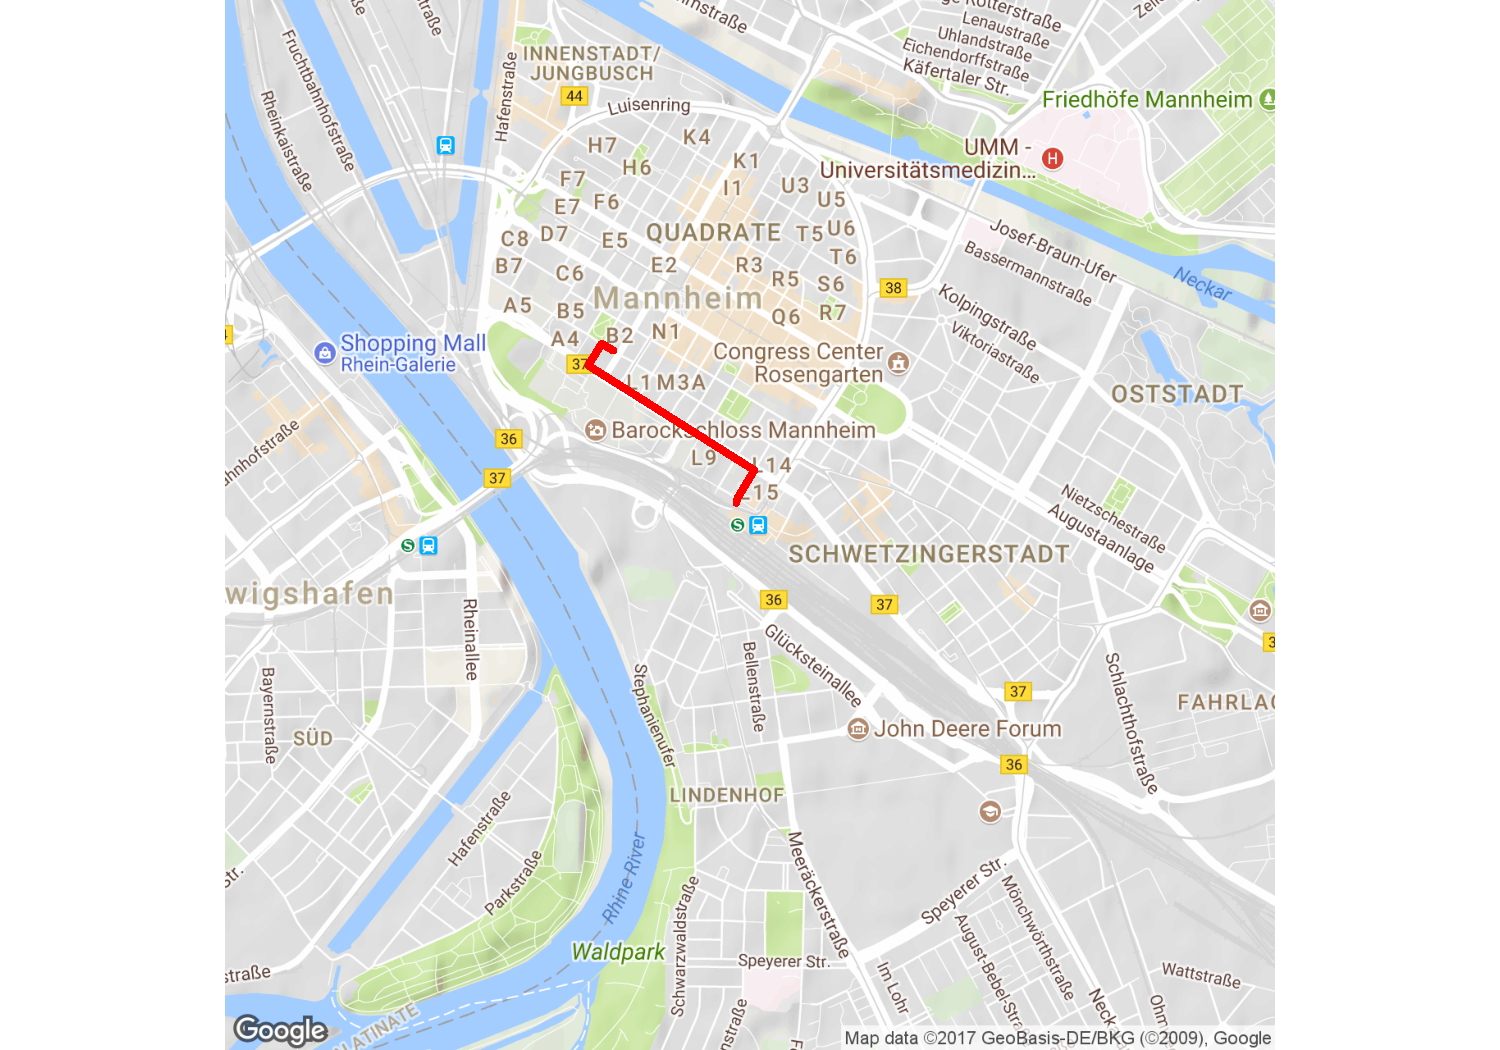
\includegraphics{RSocialScience2_files/figure-beamer/unnamed-chunk-60-1.pdf}
\caption{}
\end{figure}

Wie fügt man Punkte hinzu

\begin{itemize}
\item
  Nutzung von
  \href{http://zevross.com/blog/2014/07/16/mapping-in-r-using-the-ggplot2-package/}{geom\_point}
\item
  Frage auf
  \href{http://stackoverflow.com/questions/15069963/getting-a-map-with-points-using-ggmap-and-ggplot2}{stackoverflow}
\end{itemize}

\end{frame}

\begin{frame}{Bubbles auf einer Karte}

\url{http://i.stack.imgur.com}

\begin{figure}[htbp]
\centering
\includegraphics{https://github.com/Japhilko/IntroR/raw/master/2017/slides/figure/q3euq.png}
\caption{}
\end{figure}

\end{frame}

\begin{frame}{Cheatsheet}

\begin{itemize}
\tightlist
\item
  Cheatsheet zu
  \href{https://www.rstudio.com/wp-content/uploads/2015/04/ggplot2-cheatsheet.pdf}{data
  visualisation}
\end{itemize}

\url{https://www.rstudio.com/}

\begin{figure}[htbp]
\centering
\includegraphics{https://github.com/Japhilko/IntroR/raw/master/2017/slides/figure/ggplot2-cheatsheet.png}
\caption{Cheatsheet}
\end{figure}

\end{frame}

\begin{frame}[fragile]{Resourcen und Literatur}

\begin{itemize}
\item
  \href{http://journal.r-project.org/archive/2013-1/kahle-wickham.pdf}{Artikel
  von David Kahle und Hadley Wickham} zur Nutzung von \texttt{ggmap}.
\item
  \href{http://rpackages.ianhowson.com/cran/ggmap/man/get_map.html}{Schnell
  eine Karte bekommen}
\item
  \href{http://www.kevjohnson.org/making-maps-in-r-part-2/}{Karten
  machen mit R}
\item
  \href{http://stackoverflow.com/questions/40642850/ggmap-error-geomrasterann-was-built-with-an-incompatible-version-of-ggproto}{Problem
  mit der Installation von ggmap}
\end{itemize}

\end{frame}

\begin{frame}{Take Home Message}

Was klar sein sollte:

\begin{itemize}
\tightlist
\item
  Wie man eine schnelle Karte erzeugt
\item
  Wie man geokodiert
\item
  Wie man eine Distanz berechnet
\end{itemize}

\end{frame}

\begin{frame}{Die lineare Regression}

\end{frame}

\begin{frame}{Die lineare Regression}

Maindonald -
\href{https://cran.r-project.org/doc/contrib/usingR.pdf}{Data Analysis}

\begin{itemize}
\tightlist
\item
  Einführung in R
\item
  Datenanalyse
\item
  Statistische Modelle
\item
  Inferenzkonzepte
\item
  Regression mit einem Prädiktor
\item
  Multiple lineare Regression
\item
  Ausweitung des linearen Modells
\item
  \ldots{}
\end{itemize}

\end{frame}

\begin{frame}[fragile]{Lineare Regression in R - Beispieldatensatz}

John H. Maindonald and W. John Braun

DAAG -
\href{http://cran.ms.unimelb.edu.au/web/packages/DAAG/DAAG.pdf}{Data
Analysis and Graphics Data and Functions}

\begin{Shaded}
\begin{Highlighting}[]
\KeywordTok{install.packages}\NormalTok{(}\StringTok{"DAAG"}\NormalTok{)}
\end{Highlighting}
\end{Shaded}

\begin{Shaded}
\begin{Highlighting}[]
\KeywordTok{library}\NormalTok{(}\StringTok{"DAAG"}\NormalTok{)}
\KeywordTok{data}\NormalTok{(roller)}
\end{Highlighting}
\end{Shaded}

help on roller data:

\begin{Shaded}
\begin{Highlighting}[]
\NormalTok{?roller}
\end{Highlighting}
\end{Shaded}

\end{frame}

\begin{frame}[fragile]{Das lineare Regressionsmodell in R}

Schätzen eines Regressionsmodells:

\begin{Shaded}
\begin{Highlighting}[]
\NormalTok{roller.lm <-}\StringTok{ }\KeywordTok{lm}\NormalTok{(depression ~}\StringTok{ }\NormalTok{weight, }\DataTypeTok{data =} \NormalTok{roller)}
\end{Highlighting}
\end{Shaded}

So bekommt man die Schätzwerte:

\begin{Shaded}
\begin{Highlighting}[]
\KeywordTok{summary}\NormalTok{(roller.lm)}
\end{Highlighting}
\end{Shaded}

\begin{verbatim}
## 
## Call:
## lm(formula = depression ~ weight, data = roller)
## 
## Residuals:
##    Min     1Q Median     3Q    Max 
## -8.180 -5.580 -1.346  5.920  8.020 
## 
## Coefficients:
##             Estimate Std. Error t value Pr(>|t|)   
## (Intercept)  -2.0871     4.7543  -0.439  0.67227   
## weight        2.6667     0.7002   3.808  0.00518 **
## ---
## Signif. codes:  0 '***' 0.001 '**' 0.01 '*' 0.05 '.' 0.1 ' ' 1
## 
## Residual standard error: 6.735 on 8 degrees of freedom
## Multiple R-squared:  0.6445, Adjusted R-squared:  0.6001 
## F-statistic:  14.5 on 1 and 8 DF,  p-value: 0.005175
\end{verbatim}

Falls das Modell ohne Intercept gesch?tzt werden soll:

\begin{Shaded}
\begin{Highlighting}[]
\KeywordTok{lm}\NormalTok{(depression ~}\StringTok{ }\NormalTok{-}\DecValTok{1} \NormalTok{+}\StringTok{ }\NormalTok{weight, }\DataTypeTok{data =} \NormalTok{roller)}
\end{Highlighting}
\end{Shaded}

\begin{verbatim}
## 
## Call:
## lm(formula = depression ~ -1 + weight, data = roller)
## 
## Coefficients:
## weight  
##  2.392
\end{verbatim}

\end{frame}

\begin{frame}[fragile]{Summary des Modells}

\begin{Shaded}
\begin{Highlighting}[]
\KeywordTok{summary}\NormalTok{(roller.lm)}
\end{Highlighting}
\end{Shaded}

\begin{verbatim}
## 
## Call:
## lm(formula = depression ~ weight, data = roller)
## 
## Residuals:
##    Min     1Q Median     3Q    Max 
## -8.180 -5.580 -1.346  5.920  8.020 
## 
## Coefficients:
##             Estimate Std. Error t value Pr(>|t|)   
## (Intercept)  -2.0871     4.7543  -0.439  0.67227   
## weight        2.6667     0.7002   3.808  0.00518 **
## ---
## Signif. codes:  0 '***' 0.001 '**' 0.01 '*' 0.05 '.' 0.1 ' ' 1
## 
## Residual standard error: 6.735 on 8 degrees of freedom
## Multiple R-squared:  0.6445, Adjusted R-squared:  0.6001 
## F-statistic:  14.5 on 1 and 8 DF,  p-value: 0.005175
\end{verbatim}

\end{frame}

\begin{frame}[fragile]{R arbeitet mit Objekten}

\begin{itemize}
\tightlist
\item
  \texttt{roller.lm} ist nun ein spezielles Regressions-Objekt
\item
  Auf dieses Objekt können nun verschiedene Funktionen angewendet werden
\end{itemize}

\begin{Shaded}
\begin{Highlighting}[]
\KeywordTok{predict}\NormalTok{(roller.lm) }\CommentTok{# Vorhersage}
\end{Highlighting}
\end{Shaded}

\begin{verbatim}
##         1         2         3         4         5         6         7 
##  2.979669  6.179765  6.713114 10.713233 12.046606 14.180002 14.980026 
##         8         9        10 
## 18.180121 24.046962 30.980502
\end{verbatim}

\begin{Shaded}
\begin{Highlighting}[]
\KeywordTok{resid}\NormalTok{(roller.lm) }\CommentTok{# Residuen}
\end{Highlighting}
\end{Shaded}

\begin{verbatim}
##          1          2          3          4          5          6 
## -0.9796695 -5.1797646 -1.7131138 -5.7132327  7.9533944  5.8199976 
##          7          8          9         10 
##  8.0199738 -8.1801213  5.9530377 -5.9805017
\end{verbatim}

\end{frame}

\begin{frame}[fragile]{Residuenplot}

\begin{itemize}
\tightlist
\item
  Sind Annahmen des linearen Regressionsmodells verletzt?
\item
  Dies ist der Fall, wenn ein Muster abweichend von einer Linie zu
  erkennen ist.
\item
  Hier ist der Datensatz sehr klein
\end{itemize}

\begin{Shaded}
\begin{Highlighting}[]
\KeywordTok{plot}\NormalTok{(roller.lm,}\DecValTok{1}\NormalTok{)}
\end{Highlighting}
\end{Shaded}

\begin{figure}[htbp]
\centering
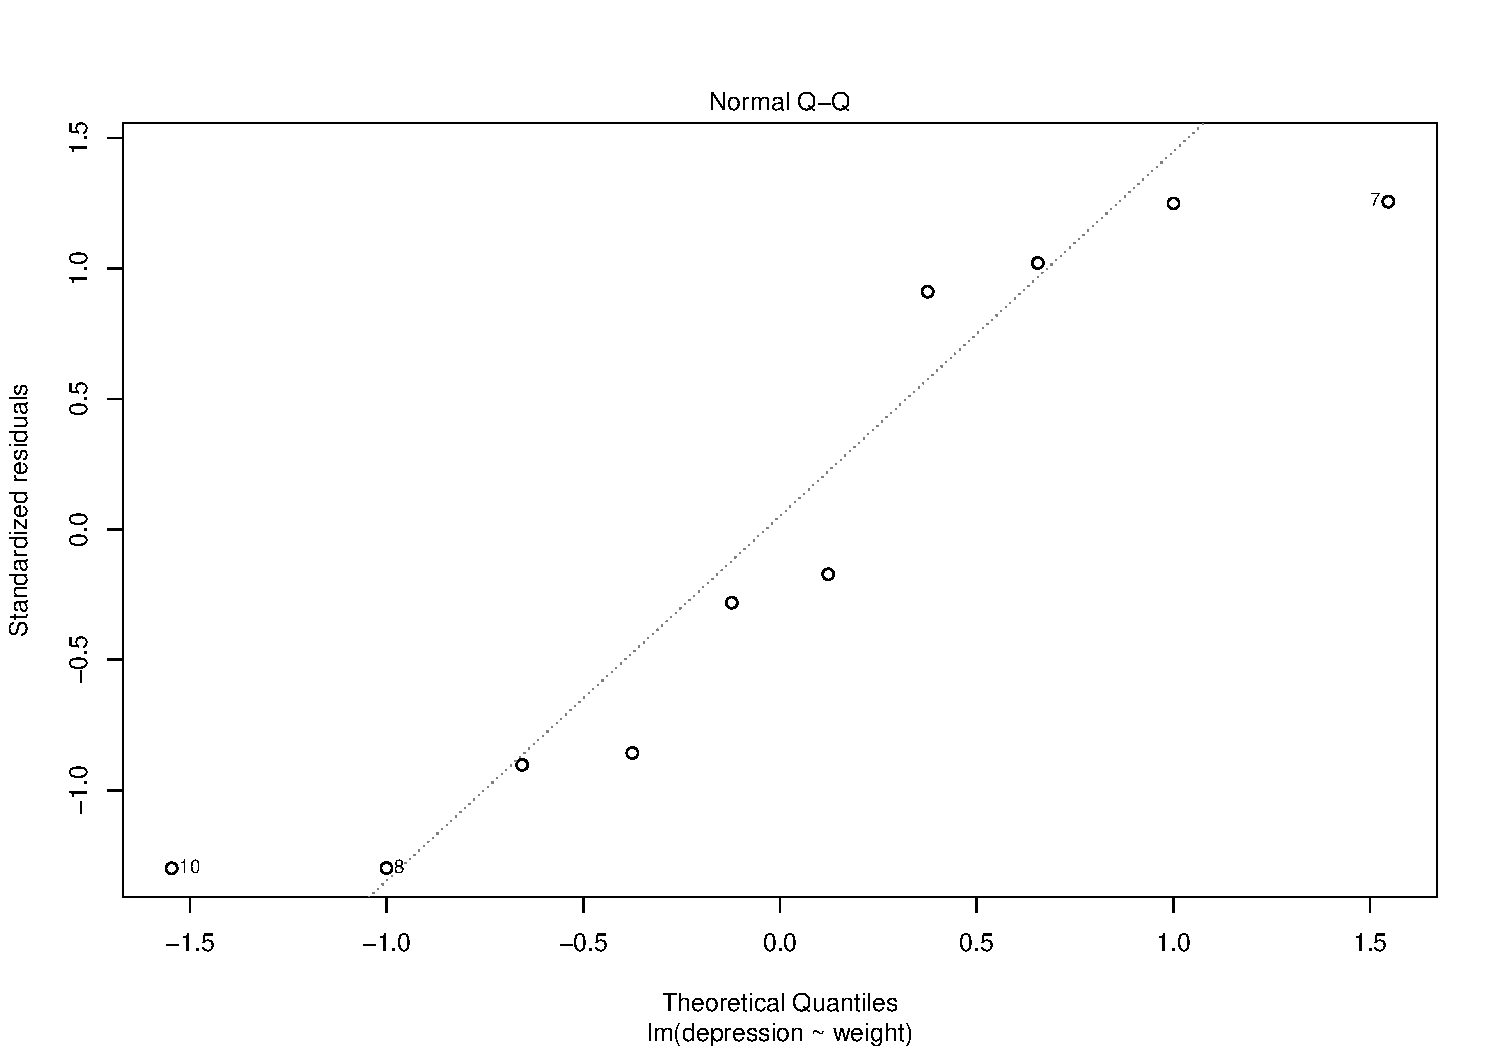
\includegraphics{RSocialScience2_files/figure-beamer/unnamed-chunk-70-1.pdf}
\caption{}
\end{figure}

\end{frame}

\begin{frame}[fragile]{Residuenplot}

\begin{itemize}
\tightlist
\item
  Wenn die Residuen normalverteilt sind sollten sie auf einer Linie
  liegen.
\end{itemize}

\begin{Shaded}
\begin{Highlighting}[]
\KeywordTok{plot}\NormalTok{(roller.lm,}\DecValTok{2}\NormalTok{)}
\end{Highlighting}
\end{Shaded}

\begin{figure}[htbp]
\centering
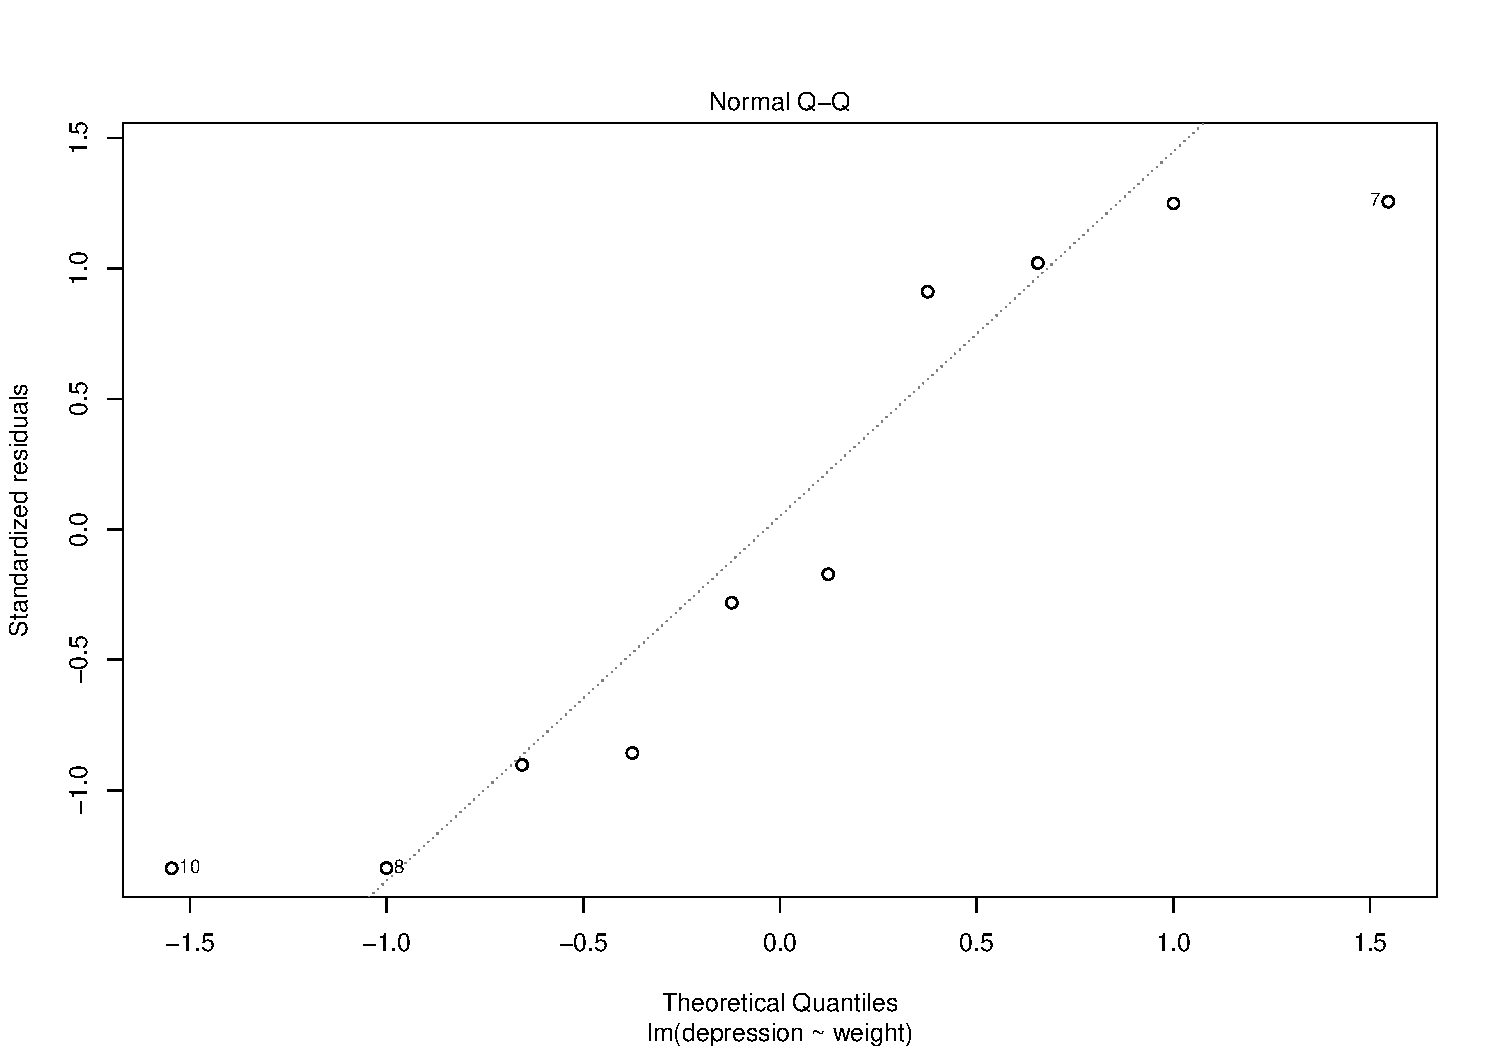
\includegraphics{RSocialScience2_files/figure-beamer/unnamed-chunk-71-1.pdf}
\caption{}
\end{figure}

\end{frame}

\begin{frame}[fragile]{Regressionsdiagnostik mit Basis-R}

Ein einfaches Modell

\begin{Shaded}
\begin{Highlighting}[]
\NormalTok{N <-}\StringTok{ }\DecValTok{5}
\NormalTok{x1 <-}\StringTok{ }\KeywordTok{rnorm}\NormalTok{(N)}
\NormalTok{y <-}\StringTok{ }\KeywordTok{runif}\NormalTok{(N)}
\end{Highlighting}
\end{Shaded}

\end{frame}

\begin{frame}[fragile]{Die Dichte der beiden Vektoren}

\begin{Shaded}
\begin{Highlighting}[]
\KeywordTok{par}\NormalTok{(}\DataTypeTok{mfrow=}\KeywordTok{c}\NormalTok{(}\DecValTok{1}\NormalTok{,}\DecValTok{2}\NormalTok{))}
\KeywordTok{plot}\NormalTok{(}\KeywordTok{density}\NormalTok{(x1))}
\KeywordTok{plot}\NormalTok{(}\KeywordTok{density}\NormalTok{(y))}
\end{Highlighting}
\end{Shaded}

\begin{figure}[htbp]
\centering
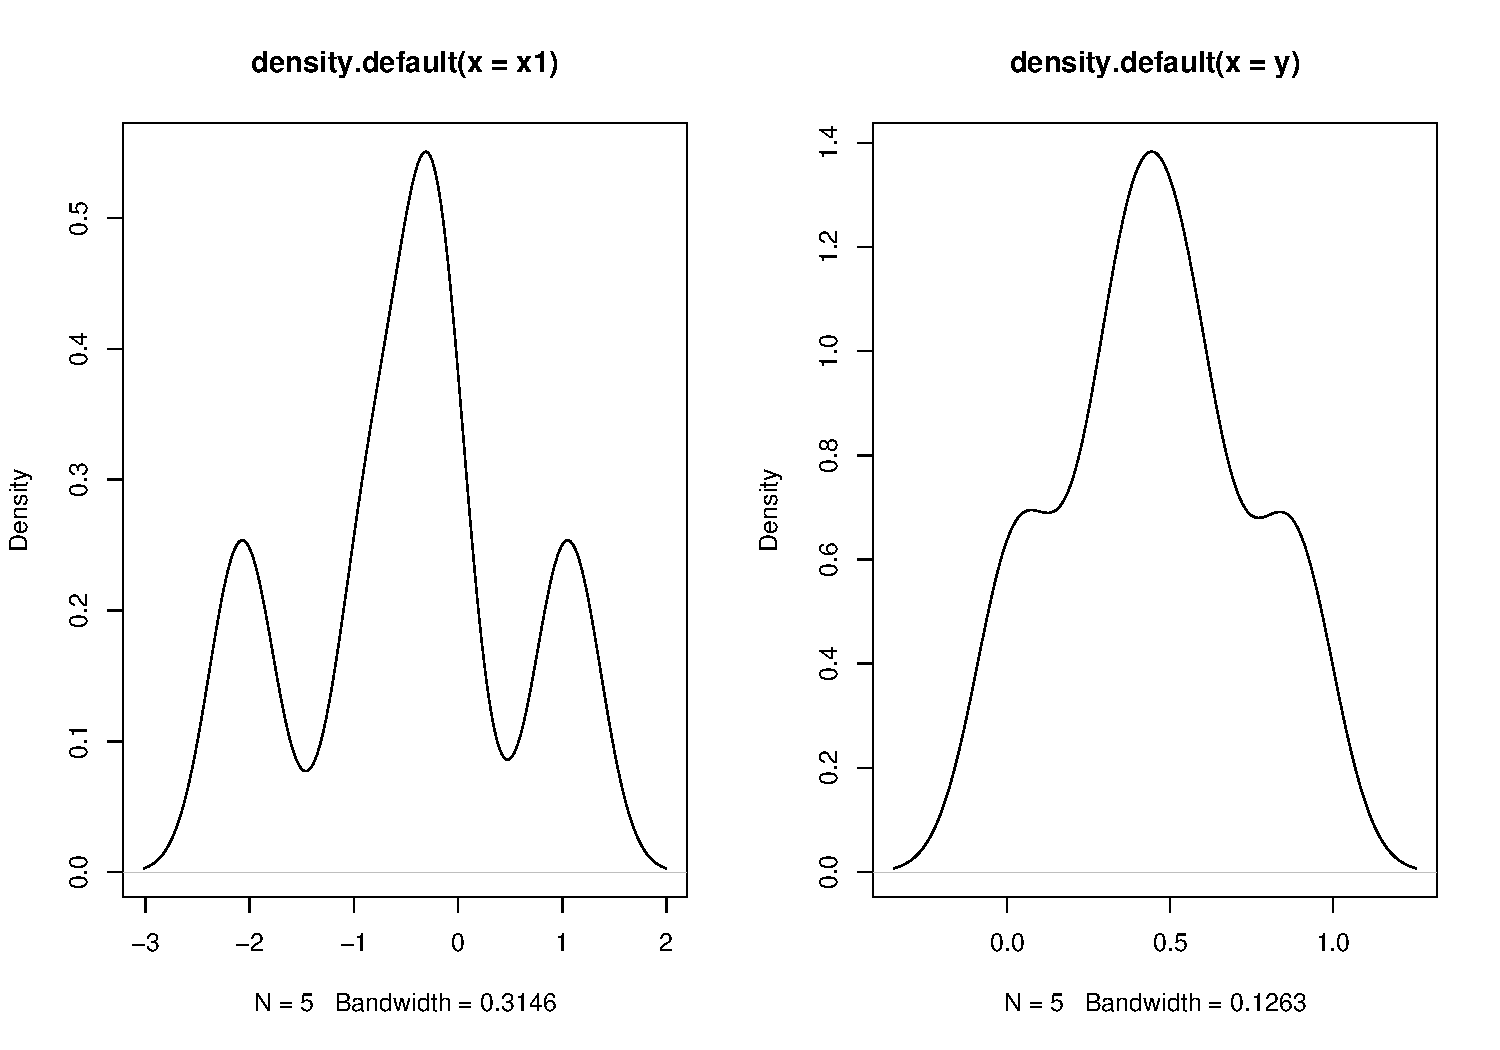
\includegraphics{RSocialScience2_files/figure-beamer/unnamed-chunk-73-1.pdf}
\caption{}
\end{figure}

\end{frame}

\begin{frame}[fragile]{Modellvorhersage machen}

\begin{Shaded}
\begin{Highlighting}[]
\NormalTok{mod1 <-}\StringTok{ }\KeywordTok{lm}\NormalTok{(y~x1)}
\NormalTok{pre <-}\StringTok{ }\KeywordTok{predict}\NormalTok{(mod1)}
\NormalTok{y}
\end{Highlighting}
\end{Shaded}

\begin{verbatim}
## [1] 0.2710050 0.7564149 0.0460009 0.5628672 0.5519674
\end{verbatim}

\begin{Shaded}
\begin{Highlighting}[]
\NormalTok{pre}
\end{Highlighting}
\end{Shaded}

\begin{verbatim}
##         1         2         3         4         5 
## 0.3748280 0.4585398 0.4500227 0.3814526 0.5234123
\end{verbatim}

\end{frame}

\begin{frame}[fragile]{Regressionsdiagnostik mit Basis-R}

\begin{Shaded}
\begin{Highlighting}[]
\KeywordTok{plot}\NormalTok{(x1,y)}
\KeywordTok{abline}\NormalTok{(mod1)}
\KeywordTok{segments}\NormalTok{(x1, y, x1, pre, }\DataTypeTok{col=}\StringTok{"red"}\NormalTok{)}
\end{Highlighting}
\end{Shaded}

\begin{figure}[htbp]
\centering
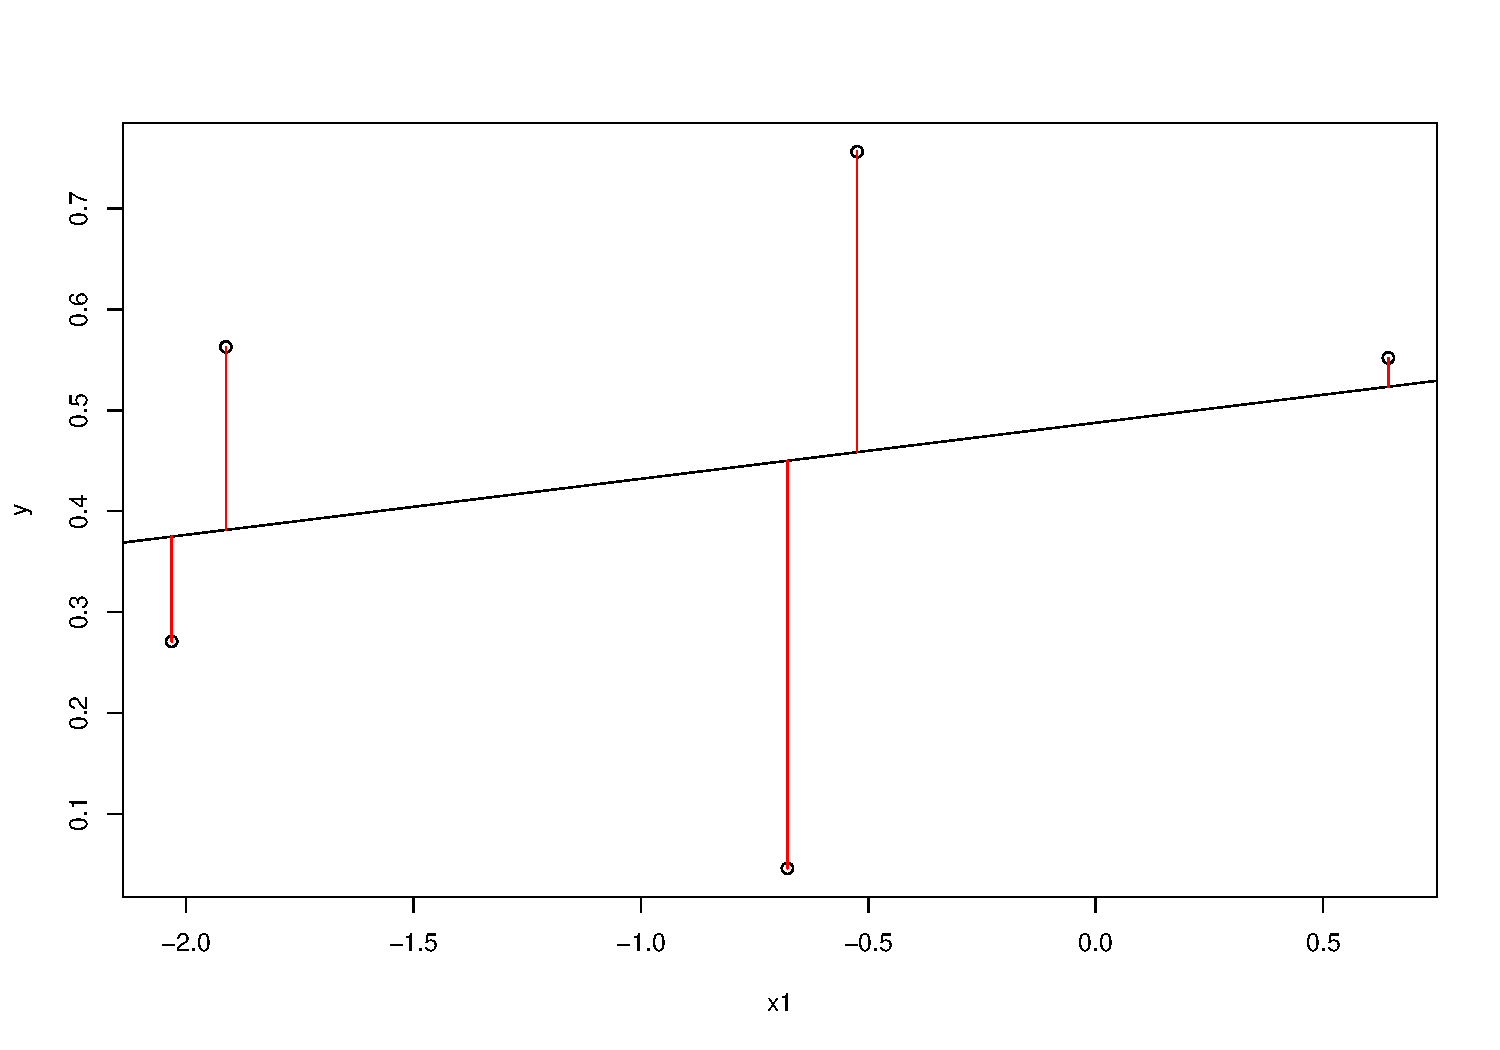
\includegraphics{RSocialScience2_files/figure-beamer/unnamed-chunk-75-1.pdf}
\caption{}
\end{figure}

\end{frame}

\begin{frame}[fragile]{Beispieldaten Luftqualität}

\begin{Shaded}
\begin{Highlighting}[]
\KeywordTok{library}\NormalTok{(datasets)}
\NormalTok{?airquality}
\end{Highlighting}
\end{Shaded}

\begin{figure}[htbp]
\centering
\includegraphics{https://github.com/Japhilko/IntroR/raw/master/2017/slides/figure/DataAirquality.PNG}
\caption{}
\end{figure}

\end{frame}

\begin{frame}[fragile]{Das \texttt{visreg}-Paket}

Ein Modell wird auf dem airquality Datensatz geschätzt

\begin{Shaded}
\begin{Highlighting}[]
\KeywordTok{install.packages}\NormalTok{(}\StringTok{"visreg"}\NormalTok{)}
\end{Highlighting}
\end{Shaded}

\begin{Shaded}
\begin{Highlighting}[]
\KeywordTok{library}\NormalTok{(visreg)}
\NormalTok{fit <-}\StringTok{ }\KeywordTok{lm}\NormalTok{(Ozone ~}\StringTok{ }\NormalTok{Solar.R +}\StringTok{ }\NormalTok{Wind +}\StringTok{ }\NormalTok{Temp, }\DataTypeTok{data =} \NormalTok{airquality)}
\KeywordTok{summary}\NormalTok{(fit)}
\end{Highlighting}
\end{Shaded}

\begin{verbatim}
## 
## Call:
## lm(formula = Ozone ~ Solar.R + Wind + Temp, data = airquality)
## 
## Residuals:
##     Min      1Q  Median      3Q     Max 
## -40.485 -14.219  -3.551  10.097  95.619 
## 
## Coefficients:
##              Estimate Std. Error t value Pr(>|t|)    
## (Intercept) -64.34208   23.05472  -2.791  0.00623 ** 
## Solar.R       0.05982    0.02319   2.580  0.01124 *  
## Wind         -3.33359    0.65441  -5.094 1.52e-06 ***
## Temp          1.65209    0.25353   6.516 2.42e-09 ***
## ---
## Signif. codes:  0 '***' 0.001 '**' 0.01 '*' 0.05 '.' 0.1 ' ' 1
## 
## Residual standard error: 21.18 on 107 degrees of freedom
##   (42 observations deleted due to missingness)
## Multiple R-squared:  0.6059, Adjusted R-squared:  0.5948 
## F-statistic: 54.83 on 3 and 107 DF,  p-value: < 2.2e-16
\end{verbatim}

\end{frame}

\begin{frame}[fragile]{Visualisierung}

\begin{Shaded}
\begin{Highlighting}[]
\KeywordTok{par}\NormalTok{(}\DataTypeTok{mfrow=}\KeywordTok{c}\NormalTok{(}\DecValTok{2}\NormalTok{,}\DecValTok{2}\NormalTok{))}
\KeywordTok{visreg}\NormalTok{(fit)}
\end{Highlighting}
\end{Shaded}

\begin{figure}[htbp]
\centering
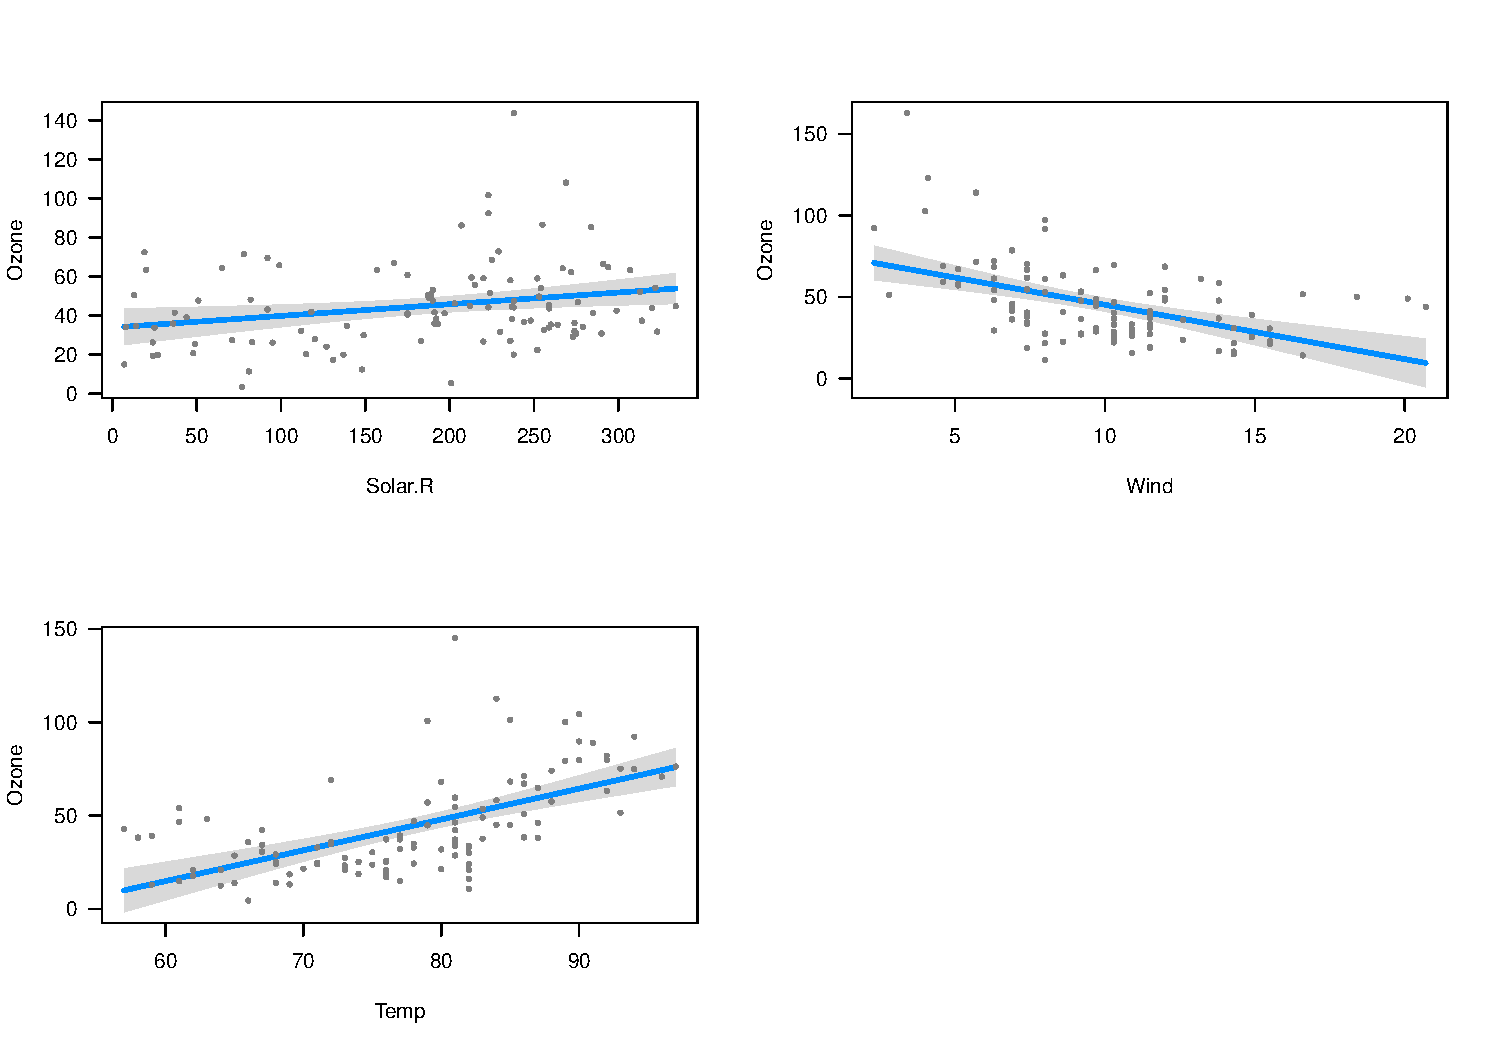
\includegraphics{RSocialScience2_files/figure-beamer/unnamed-chunk-79-1.pdf}
\caption{}
\end{figure}

\end{frame}

\begin{frame}[fragile]{\href{http://myweb.uiowa.edu/pbreheny/publications/visreg.pdf}{Und
dann mit \texttt{visreg} visualisiert.}}

\begin{itemize}
\tightlist
\item
  Zweites Argument - Spezifikation erklärende Variable für
  Visualisierung
\end{itemize}

\begin{Shaded}
\begin{Highlighting}[]
\KeywordTok{visreg}\NormalTok{(fit, }\StringTok{"Wind"}\NormalTok{, }\DataTypeTok{type =} \StringTok{"contrast"}\NormalTok{)}
\end{Highlighting}
\end{Shaded}

\begin{figure}[htbp]
\centering
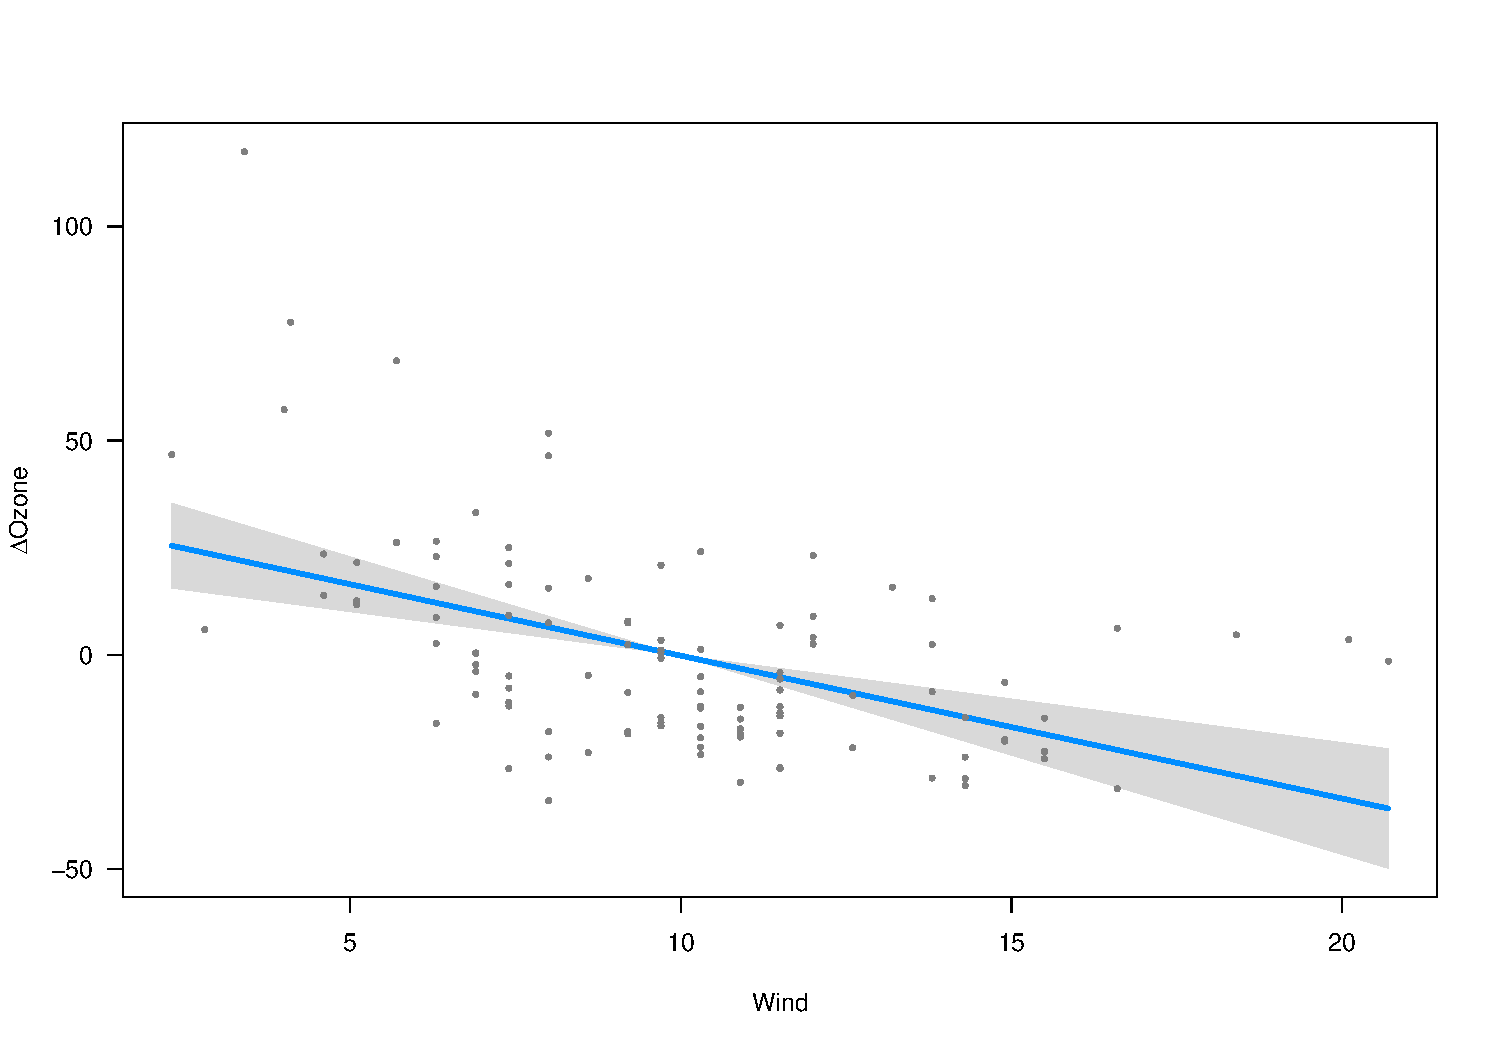
\includegraphics{RSocialScience2_files/figure-beamer/unnamed-chunk-80-1.pdf}
\caption{}
\end{figure}

\end{frame}

\begin{frame}[fragile]{Visualisierung mit dem Paket \texttt{visreg}}

\begin{Shaded}
\begin{Highlighting}[]
\KeywordTok{visreg}\NormalTok{(fit, }\StringTok{"Wind"}\NormalTok{, }\DataTypeTok{type =} \StringTok{"contrast"}\NormalTok{)}
\end{Highlighting}
\end{Shaded}

\begin{figure}[htbp]
\centering
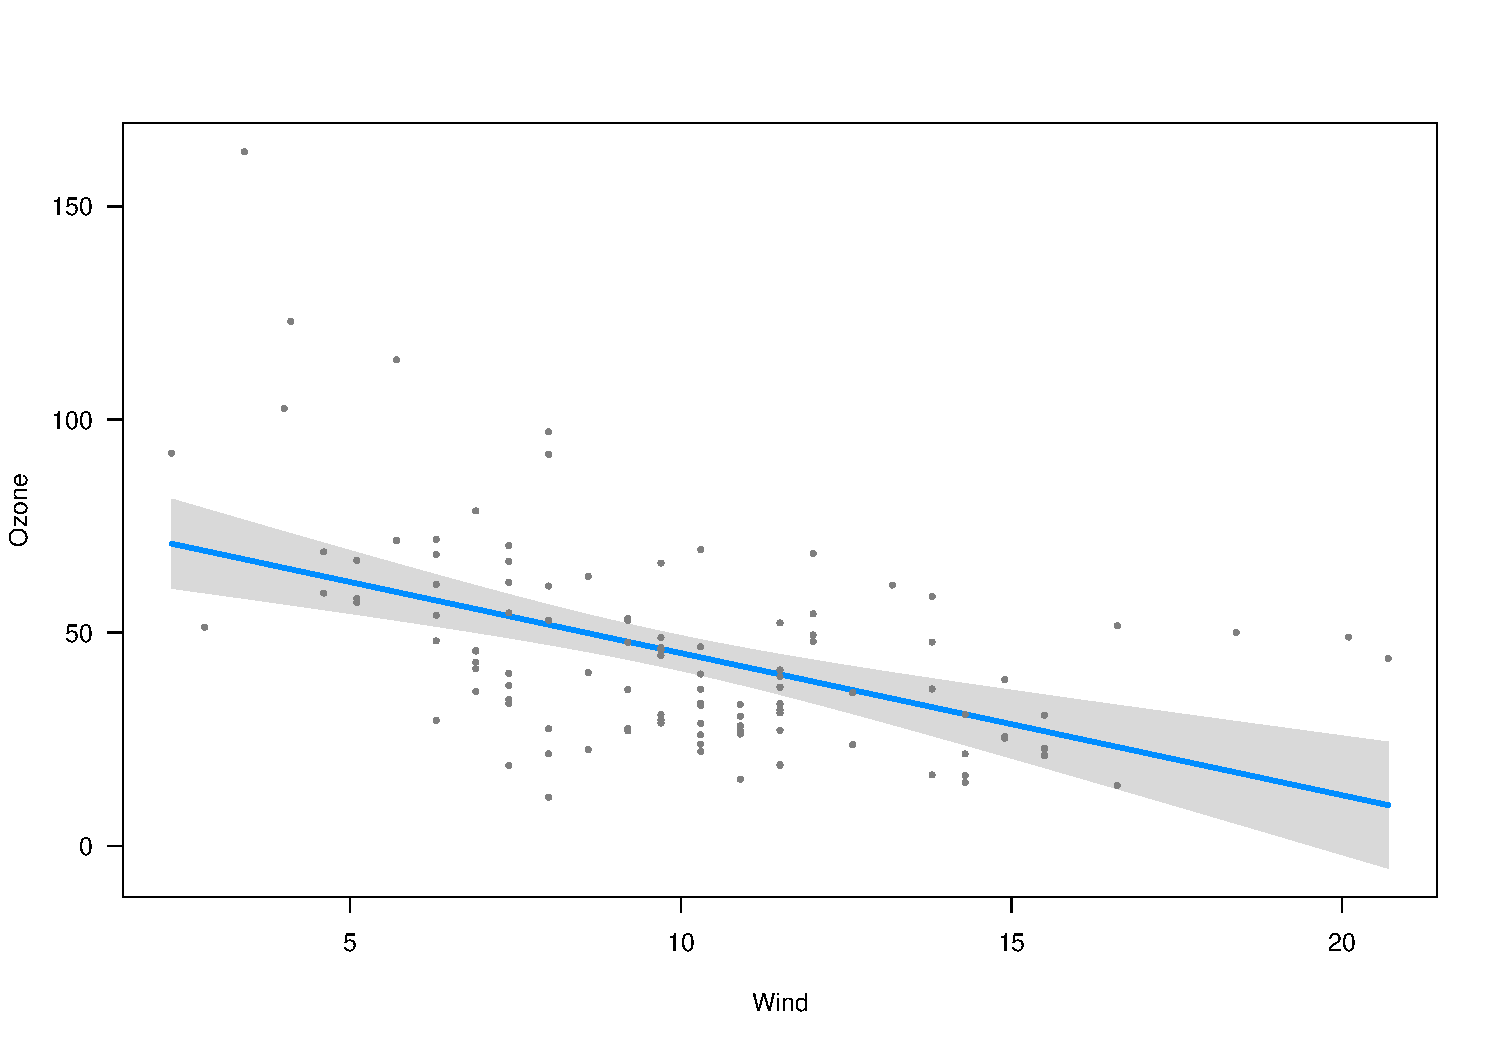
\includegraphics{RSocialScience2_files/figure-beamer/unnamed-chunk-81-1.pdf}
\caption{}
\end{figure}

\end{frame}

\begin{frame}[fragile]{Das \texttt{visreg}-Paket}

\begin{itemize}
\tightlist
\item
  Das Default-Argument für type ist conditional.
\end{itemize}

\begin{Shaded}
\begin{Highlighting}[]
\KeywordTok{visreg}\NormalTok{(fit, }\StringTok{"Wind"}\NormalTok{, }\DataTypeTok{type =} \StringTok{"conditional"}\NormalTok{)}
\end{Highlighting}
\end{Shaded}

\begin{figure}[htbp]
\centering
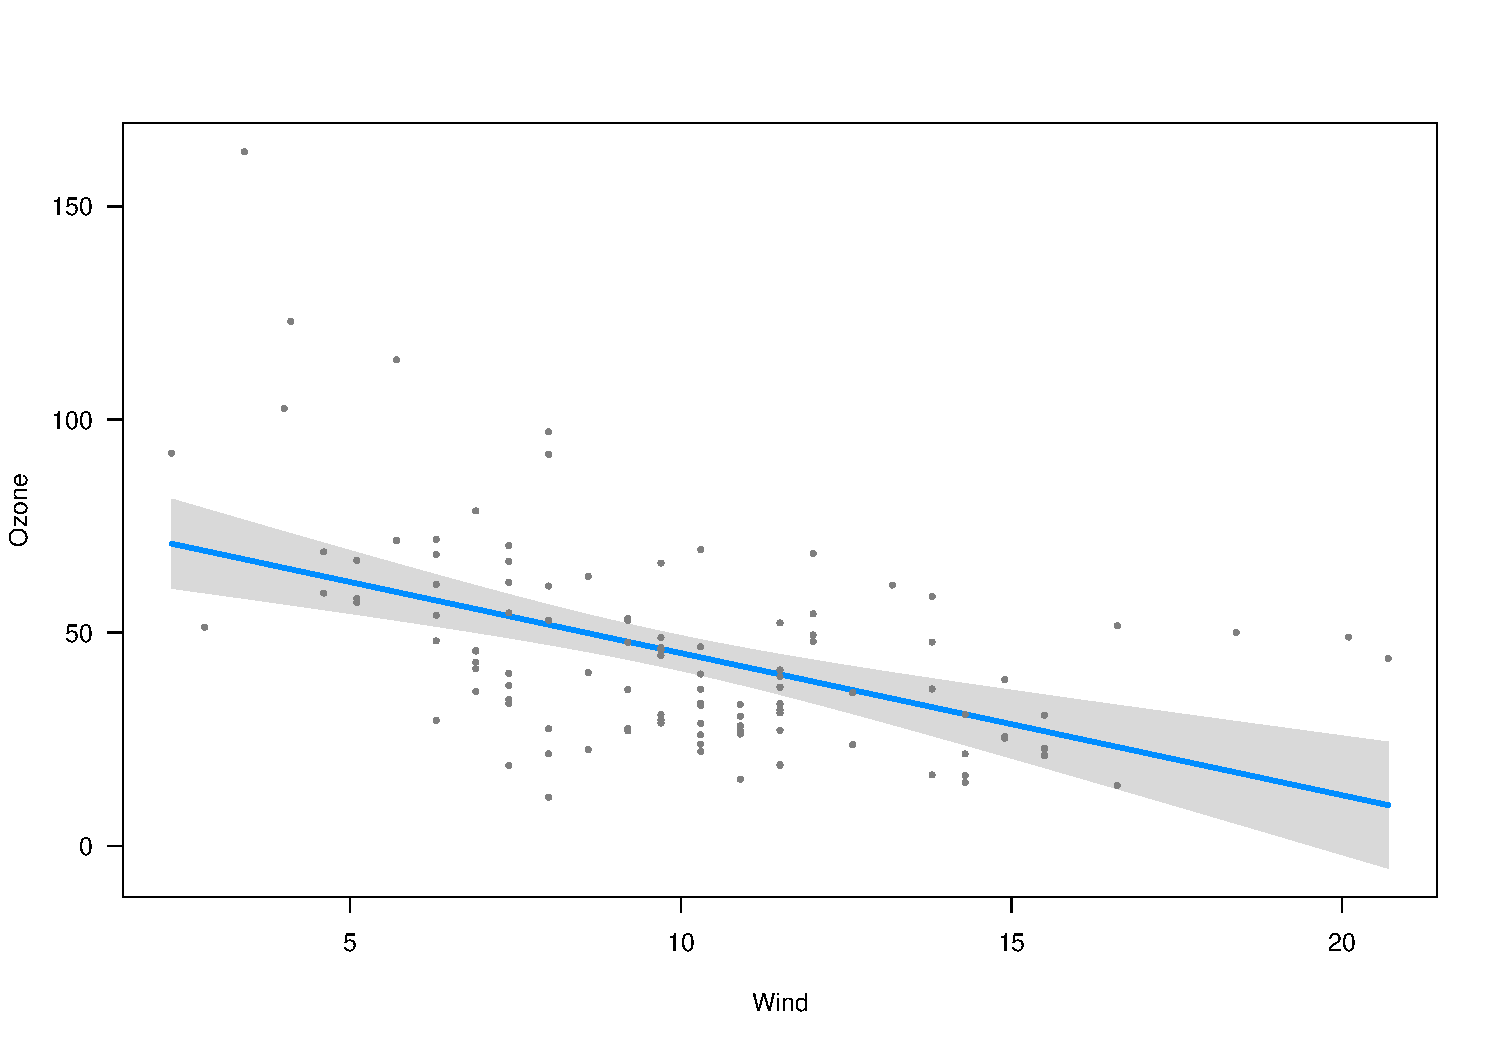
\includegraphics{RSocialScience2_files/figure-beamer/unnamed-chunk-82-1.pdf}
\caption{}
\end{figure}

\end{frame}

\begin{frame}[fragile]{Regression mit Faktoren}

Mit \texttt{visreg} können die Effekte bei Faktoren visualisiert werden.

\begin{Shaded}
\begin{Highlighting}[]
\NormalTok{airquality$Heat <-}\StringTok{ }\KeywordTok{cut}\NormalTok{(airquality$Temp, }\DecValTok{3}\NormalTok{, }
    \DataTypeTok{labels=}\KeywordTok{c}\NormalTok{(}\StringTok{"Cool"}\NormalTok{, }\StringTok{"Mild"}\NormalTok{, }\StringTok{"Hot"}\NormalTok{))}
\NormalTok{fit.heat <-}\StringTok{ }\KeywordTok{lm}\NormalTok{(Ozone ~}\StringTok{ }\NormalTok{Solar.R +}\StringTok{ }\NormalTok{Wind +}\StringTok{ }\NormalTok{Heat, }
    \DataTypeTok{data =} \NormalTok{airquality)}
\KeywordTok{summary}\NormalTok{(fit.heat)}
\end{Highlighting}
\end{Shaded}

\begin{verbatim}
## 
## Call:
## lm(formula = Ozone ~ Solar.R + Wind + Heat, data = airquality)
## 
## Residuals:
##     Min      1Q  Median      3Q     Max 
## -33.473 -12.794  -2.686   8.461 107.035 
## 
## Coefficients:
##             Estimate Std. Error t value Pr(>|t|)    
## (Intercept) 48.27682    8.83072   5.467 3.07e-07 ***
## Solar.R      0.06524    0.02145   3.042  0.00296 ** 
## Wind        -3.49803    0.59042  -5.925 3.94e-08 ***
## HeatMild     9.05367    4.88257   1.854  0.06648 .  
## HeatHot     43.13970    5.98618   7.207 8.79e-11 ***
## ---
## Signif. codes:  0 '***' 0.001 '**' 0.01 '*' 0.05 '.' 0.1 ' ' 1
## 
## Residual standard error: 19.9 on 106 degrees of freedom
##   (42 observations deleted due to missingness)
## Multiple R-squared:  0.6554, Adjusted R-squared:  0.6424 
## F-statistic:  50.4 on 4 and 106 DF,  p-value: < 2.2e-16
\end{verbatim}

\end{frame}

\begin{frame}[fragile]{Effekte von Faktoren}

\begin{Shaded}
\begin{Highlighting}[]
\KeywordTok{par}\NormalTok{(}\DataTypeTok{mfrow=}\KeywordTok{c}\NormalTok{(}\DecValTok{1}\NormalTok{,}\DecValTok{2}\NormalTok{))}
\KeywordTok{visreg}\NormalTok{(fit.heat, }\StringTok{"Heat"}\NormalTok{, }\DataTypeTok{type =} \StringTok{"contrast"}\NormalTok{)}
\KeywordTok{visreg}\NormalTok{(fit.heat, }\StringTok{"Heat"}\NormalTok{, }\DataTypeTok{type =} \StringTok{"conditional"}\NormalTok{)}
\end{Highlighting}
\end{Shaded}

\begin{figure}[htbp]
\centering
\includegraphics{RSocialScience2_files/figure-beamer/unnamed-chunk-84-1.pdf}
\caption{}
\end{figure}

\end{frame}

\begin{frame}[fragile]{Das Paket visreg - Interaktionen}

\begin{Shaded}
\begin{Highlighting}[]
\NormalTok{airquality$Heat <-}\StringTok{ }\KeywordTok{cut}\NormalTok{(airquality$Temp, }\DecValTok{3}\NormalTok{, }
\DataTypeTok{labels=}\KeywordTok{c}\NormalTok{(}\StringTok{"Cool"}\NormalTok{, }\StringTok{"Mild"}\NormalTok{, }\StringTok{"Hot"}\NormalTok{))}
\NormalTok{fit <-}\StringTok{ }\KeywordTok{lm}\NormalTok{(Ozone ~}\StringTok{ }\NormalTok{Solar.R +}\StringTok{ }\NormalTok{Wind *}\StringTok{ }\NormalTok{Heat, }\DataTypeTok{data =} \NormalTok{airquality)}
\KeywordTok{summary}\NormalTok{(fit)}
\end{Highlighting}
\end{Shaded}

\begin{verbatim}
## 
## Call:
## lm(formula = Ozone ~ Solar.R + Wind * Heat, data = airquality)
## 
## Residuals:
##     Min      1Q  Median      3Q     Max 
## -34.472 -11.640  -1.919   7.403 102.428 
## 
## Coefficients:
##               Estimate Std. Error t value Pr(>|t|)    
## (Intercept)    4.48042   17.38219   0.258 0.797102    
## Solar.R        0.07634    0.02137   3.572 0.000538 ***
## Wind           0.05854    1.34860   0.043 0.965458    
## HeatMild      56.72928   18.53110   3.061 0.002805 ** 
## HeatHot       94.68619   18.61619   5.086 1.63e-06 ***
## Wind:HeatMild -4.11933    1.57108  -2.622 0.010054 *  
## Wind:HeatHot  -4.88125    1.74358  -2.800 0.006101 ** 
## ---
## Signif. codes:  0 '***' 0.001 '**' 0.01 '*' 0.05 '.' 0.1 ' ' 1
## 
## Residual standard error: 19.28 on 104 degrees of freedom
##   (42 observations deleted due to missingness)
## Multiple R-squared:  0.6825, Adjusted R-squared:  0.6642 
## F-statistic: 37.26 on 6 and 104 DF,  p-value: < 2.2e-16
\end{verbatim}

\end{frame}

\begin{frame}[fragile]{Steuern der Graphikausgabe mittels
\texttt{layout}}

\begin{Shaded}
\begin{Highlighting}[]
\KeywordTok{visreg}\NormalTok{(fit, }\StringTok{"Wind"}\NormalTok{, }\DataTypeTok{by =} \StringTok{"Heat"}\NormalTok{,}\DataTypeTok{layout=}\KeywordTok{c}\NormalTok{(}\DecValTok{3}\NormalTok{,}\DecValTok{1}\NormalTok{))}
\end{Highlighting}
\end{Shaded}

\begin{figure}[htbp]
\centering
\includegraphics{RSocialScience2_files/figure-beamer/unnamed-chunk-86-1.pdf}
\caption{}
\end{figure}

\end{frame}

\begin{frame}[fragile]{Das Paket \texttt{visreg} - Interaktionen
overlay}

\begin{Shaded}
\begin{Highlighting}[]
\NormalTok{fit<-}\KeywordTok{lm}\NormalTok{(Ozone~Solar.R+Wind*Heat,}\DataTypeTok{data=}\NormalTok{airquality)}
\KeywordTok{visreg}\NormalTok{(fit,}\StringTok{"Wind"}\NormalTok{,}\DataTypeTok{by=}\StringTok{"Heat"}\NormalTok{,}\DataTypeTok{overlay=}\OtherTok{TRUE}\NormalTok{,}\DataTypeTok{partial=}\OtherTok{FALSE}\NormalTok{)}
\end{Highlighting}
\end{Shaded}

\begin{figure}[htbp]
\centering
\includegraphics{RSocialScience2_files/figure-beamer/unnamed-chunk-87-1.pdf}
\caption{}
\end{figure}

\end{frame}

\begin{frame}[fragile]{Das Paket \texttt{visreg} - \texttt{visreg2d}}

\begin{Shaded}
\begin{Highlighting}[]
\NormalTok{fit2<-}\KeywordTok{lm}\NormalTok{(Ozone~Solar.R+Wind*Temp,}\DataTypeTok{data=}\NormalTok{airquality)}
\KeywordTok{visreg2d}\NormalTok{(fit2,}\StringTok{"Wind"}\NormalTok{,}\StringTok{"Temp"}\NormalTok{,}\DataTypeTok{plot.type=}\StringTok{"image"}\NormalTok{)}
\end{Highlighting}
\end{Shaded}

\begin{figure}[htbp]
\centering
\includegraphics{RSocialScience2_files/figure-beamer/unnamed-chunk-88-1.pdf}
\caption{}
\end{figure}

\end{frame}

\begin{frame}[fragile]{Das Paket visreg - surface}

\begin{Shaded}
\begin{Highlighting}[]
\KeywordTok{visreg2d}\NormalTok{(fit2, }\StringTok{"Wind"}\NormalTok{, }\StringTok{"Temp"}\NormalTok{, }\DataTypeTok{plot.type =} \StringTok{"persp"}\NormalTok{)}
\end{Highlighting}
\end{Shaded}

\begin{figure}[htbp]
\centering
\includegraphics{RSocialScience2_files/figure-beamer/unnamed-chunk-89-1.pdf}
\caption{}
\end{figure}

\end{frame}

\begin{frame}[fragile]{Regression mit dem \texttt{survey} Paket}

\begin{Shaded}
\begin{Highlighting}[]
\KeywordTok{library}\NormalTok{(survey)}
\KeywordTok{data}\NormalTok{(api)}
\KeywordTok{head}\NormalTok{(apipop)}
\end{Highlighting}
\end{Shaded}

\begin{verbatim}
##              cds stype            name                      sname snum
## 1 01611190130229     H    Alameda High               Alameda High    1
## 2 01611190132878     H    Encinal High               Encinal High    2
## 3 01611196000004     M  Chipman Middle             Chipman Middle    3
## 4 01611196090005     E Lum (Donald D.) Lum (Donald D.) Elementary    4
## 5 01611196090013     E Edison Elementa          Edison Elementary    5
## 6 01611196090021     E Otis (Frank) El    Otis (Frank) Elementary    6
##                  dname dnum   cname cnum flag pcttest api00 api99 target
## 1 Alameda City Unified    6 Alameda    1   NA      96   731   693      5
## 2 Alameda City Unified    6 Alameda    1   NA      99   622   589     11
## 3 Alameda City Unified    6 Alameda    1   NA      99   622   572     11
## 4 Alameda City Unified    6 Alameda    1   NA      99   774   732      3
## 5 Alameda City Unified    6 Alameda    1   NA      99   811   784      1
## 6 Alameda City Unified    6 Alameda    1   NA     100   780   725      4
##   growth sch.wide comp.imp both awards meals ell yr.rnd mobility acs.k3
## 1     38      Yes      Yes  Yes    Yes    14  16   <NA>        9     NA
## 2     33      Yes       No   No     No    20  18   <NA>       13     NA
## 3     50      Yes      Yes  Yes    Yes    55  25   <NA>       20     NA
## 4     42      Yes      Yes  Yes    Yes    35  26   <NA>       21     20
## 5     27      Yes      Yes  Yes    Yes    15   9   <NA>       11     20
## 6     55      Yes      Yes  Yes    Yes    25  18   <NA>       12     20
##   acs.46 acs.core pct.resp not.hsg hsg some.col col.grad grad.sch avg.ed
## 1     NA       25       91       6  16       22       38       18   3.45
## 2     NA       27       84      11  20       29       31        9   3.06
## 3     26       27       86      11  31       30       20        8   2.82
## 4     30       NA       96       3  22       29       31       15   3.32
## 5     29       NA       96       3   9       29       26       33   3.76
## 6     29       NA       87       6  11       28       41       13   3.44
##   full emer enroll api.stu
## 1   85   16   1278    1090
## 2   90   10   1113     840
## 3   80   12    546     472
## 4   96    4    330     272
## 5   95    5    233     216
## 6   90    5    276     247
\end{verbatim}

\end{frame}

\begin{frame}[fragile]{\href{https://www.r-bloggers.com/linear-models-with-weighted-observations/}{Das
Survey Design spezifizieren}}

\begin{Shaded}
\begin{Highlighting}[]
\NormalTok{dstrat<-}\KeywordTok{svydesign}\NormalTok{(}\DataTypeTok{id=}\NormalTok{~}\DecValTok{1}\NormalTok{,}\DataTypeTok{strata=}\NormalTok{~stype, }\DataTypeTok{weights=}\NormalTok{~pw, }
                  \DataTypeTok{data=}\NormalTok{apistrat, }\DataTypeTok{fpc=}\NormalTok{~fpc)}
\end{Highlighting}
\end{Shaded}

\begin{block}{Die Regression rechnen}

\begin{Shaded}
\begin{Highlighting}[]
\KeywordTok{summary}\NormalTok{(}\KeywordTok{svyglm}\NormalTok{(api00~ell+meals+mobility, }
               \DataTypeTok{design=}\NormalTok{dstrat))}
\end{Highlighting}
\end{Shaded}

\begin{verbatim}
## 
## Call:
## svyglm(formula = api00 ~ ell + meals + mobility, design = dstrat)
## 
## Survey design:
## svydesign(id = ~1, strata = ~stype, weights = ~pw, data = apistrat, 
##     fpc = ~fpc)
## 
## Coefficients:
##             Estimate Std. Error t value Pr(>|t|)    
## (Intercept) 820.8873    10.0777  81.456   <2e-16 ***
## ell          -0.4806     0.3920  -1.226    0.222    
## meals        -3.1415     0.2839 -11.064   <2e-16 ***
## mobility      0.2257     0.3932   0.574    0.567    
## ---
## Signif. codes:  0 '***' 0.001 '**' 0.01 '*' 0.05 '.' 0.1 ' ' 1
## 
## (Dispersion parameter for gaussian family taken to be 5171.966)
## 
## Number of Fisher Scoring iterations: 2
\end{verbatim}

\end{block}

\end{frame}

\begin{frame}{Linkliste - lineare Regression}

\begin{itemize}
\item
  Regression -
  \href{http://www.r-bloggers.com/r-tutorial-series-simple-linear-regression/}{r-bloggers}
\item
  Das Komplette Buch von
  \href{http://cran.r-project.org/doc/contrib/Faraway-PRA.pdf}{Faraway}-
  sehr intuitiv geschrieben.
\item
  Gute Einführung auf
  \href{http://www.statmethods.net/stats/regression.html}{Quick-R}
\item
  \href{https://www.r-bloggers.com/multiple-regression-part-1/}{Multiple
  Regression}
\item
  Basis Regression -
  \href{https://www.r-bloggers.com/how-to-go-about-interpreting-regression-cofficients/}{How
  to go about interpreting regression cofficients}
\end{itemize}

\end{frame}

\begin{frame}[fragile]{Aufgabe - lineare Regression}

Beschrieben wird Wegstrecke, dreier Spielzeugautos die in
unterschiedlichen Winkeln Rampe herunterfuhren.

\begin{itemize}
\tightlist
\item
  angle: Winkel der Rampe
\item
  distance: Zurückgelegte Strecke des Spielzeugautos
\item
  car: Autotyp (1, 2 oder 3)
\end{itemize}

\begin{enumerate}
\def\labelenumi{(\alph{enumi})}
\item
  Lesen Sie den Datensatz \texttt{toycars} (Paket \texttt{DAAG}) in
  einen dataframe \texttt{data} ein und wandeln Sie die Variable
  \texttt{car} des Datensatzes in einen Faktor (\texttt{as.factor}) um.
\item
  Erstellen Sie drei Boxplots, die die zurückgelegte Strecke getrennt
  nach dem Faktor car darstellen.
\item
  Schätzen Sie für die Autos die Parameter des folgenden linearen
  Modells mit Hilfe der Funktion \texttt{lm()}
\end{enumerate}

\[ distance_i= \beta_0 + \beta_1 \cdot angle_i + \epsilon_i\]

\begin{enumerate}
\def\labelenumi{(\alph{enumi})}
\setcounter{enumi}{3}
\tightlist
\item
  Überprüfen Sie deskriptiv die Anpassung der drei Modelle. Deutet das
  \[ R^2 \] jeweils auf eine gute Modellanpassung hin?
\end{enumerate}

\end{frame}

\begin{frame}{Die logistische Regression}

\end{frame}

\begin{frame}{Agresti -
\href{https://mathdept.iut.ac.ir/sites/mathdept.iut.ac.ir/files/AGRESTI.PDF}{Categorical
Data Analysis (2002)}}

\begin{figure}[htbp]
\centering
\includegraphics{https://github.com/Japhilko/IntroR/raw/master/2017/slides/figure/CDAagresti.PNG}
\caption{}
\end{figure}

\begin{itemize}
\tightlist
\item
  Sehr intiutiv geschriebenes Buch
\item
  Sehr ausführliches begleitendes Skript von
  \href{http://statweb.stanford.edu/~owen/courses/306a/Splusdiscrete2.pdf}{Thompson}
\item
  Das Skript eignet sich um die kategoriale Datenanalyse
  nachzuvollziehen
\end{itemize}

\end{frame}

\begin{frame}{Faraway Bücher zu Regression in R}

\begin{figure}[htbp]
\centering
\includegraphics{https://github.com/Japhilko/IntroR/raw/master/2017/slides/figure/Faraway.PNG}
\caption{}
\end{figure}

\begin{itemize}
\item
  Logistische Regressionen gut erklärt
\item
  Beispiele mit R-code

  \begin{itemize}
  \item
    Faraway - Extending the linear model with r
  \item
    Faraway -
    \href{https://cran.r-project.org/doc/contrib/Faraway-PRA.pdf}{Practical
    Regression and Anova using R}
  \end{itemize}
\end{itemize}

\end{frame}

\begin{frame}[fragile]{Binäre AVs mit \texttt{glm}}

\begin{itemize}
\tightlist
\item
  Die \href{http://data.princeton.edu/R/glms.html}{logistische
  Regression} gehört zur Klasse der generalisierten linearen Modelle
  (GLM)
\item
  Die Funktion zur Schätzung eines Modells dieser Klasse in heißt
  \texttt{glm()}
\item
  \texttt{glm()} muss 1. ein Formel-Objekt mitgegeben werden und 2. die
  Klasse (binomial, gaussian, Gamma) samt link-Funktion (logit, probit,
  cauchit, log, cloglog)
\end{itemize}

\end{frame}

\begin{frame}[fragile]{Beispieldaten für die logistische Regression}

\begin{Shaded}
\begin{Highlighting}[]
\KeywordTok{install.packages}\NormalTok{(}\StringTok{"HSAUR"}\NormalTok{)}
\end{Highlighting}
\end{Shaded}

\begin{Shaded}
\begin{Highlighting}[]
\KeywordTok{library}\NormalTok{(}\StringTok{"HSAUR"}\NormalTok{)}
\KeywordTok{data}\NormalTok{(}\StringTok{"plasma"}\NormalTok{, }\DataTypeTok{package =} \StringTok{"HSAUR"}\NormalTok{)}
\end{Highlighting}
\end{Shaded}

\end{frame}

\begin{frame}[fragile]{Logistische Regression mit R}

\begin{itemize}
\tightlist
\item
  \href{http://homepage.univie.ac.at/herbert.nagel/KategorialeDaten.pdf}{Kategoriale
  Daten:}
\end{itemize}

\begin{Shaded}
\begin{Highlighting}[]
\KeywordTok{cdplot}\NormalTok{(ESR ~}\StringTok{ }\NormalTok{fibrinogen, }\DataTypeTok{data =} \NormalTok{plasma)}
\end{Highlighting}
\end{Shaded}

\includegraphics{RSocialScience2_files/figure-beamer/unnamed-chunk-96-1.pdf}

\end{frame}

\begin{frame}[fragile]{\href{http://ww2.coastal.edu/kingw/statistics/R-tutorials/logistic.html}{Logistische
Regression} mit R}

\begin{Shaded}
\begin{Highlighting}[]
\NormalTok{plasma_glm_1 <-}\StringTok{ }\KeywordTok{glm}\NormalTok{(ESR ~}\StringTok{ }\NormalTok{fibrinogen, }\DataTypeTok{data =} \NormalTok{plasma, }
                    \DataTypeTok{family =} \KeywordTok{binomial}\NormalTok{())}
\end{Highlighting}
\end{Shaded}

\end{frame}

\begin{frame}[fragile]{Weitere Beispieldaten}

\begin{Shaded}
\begin{Highlighting}[]
\KeywordTok{install.packages}\NormalTok{(}\StringTok{"faraway"}\NormalTok{)}
\end{Highlighting}
\end{Shaded}

\begin{Shaded}
\begin{Highlighting}[]
\KeywordTok{library}\NormalTok{(}\StringTok{"faraway"}\NormalTok{)}
\end{Highlighting}
\end{Shaded}

\begin{Shaded}
\begin{Highlighting}[]
\KeywordTok{data}\NormalTok{(orings)}
\end{Highlighting}
\end{Shaded}

\begin{longtable}[]{@{}rr@{}}
\toprule
temp & damage\tabularnewline
\midrule
\endhead
53 & 5\tabularnewline
57 & 1\tabularnewline
58 & 1\tabularnewline
\bottomrule
\end{longtable}

\end{frame}

\begin{frame}[fragile]{Generalisierte Regression mit R - weitere
Funktionen}

\begin{itemize}
\tightlist
\item
  Logistisches Modell mit Probit-Link:
\end{itemize}

\begin{Shaded}
\begin{Highlighting}[]
\NormalTok{probitmod <-}\StringTok{ }\KeywordTok{glm}\NormalTok{(}\KeywordTok{cbind}\NormalTok{(damage,}\DecValTok{6}\NormalTok{-damage) ~}\StringTok{ }\NormalTok{temp, }
    \DataTypeTok{family=}\KeywordTok{binomial}\NormalTok{(}\DataTypeTok{link=}\NormalTok{probit), orings)}
\end{Highlighting}
\end{Shaded}

\begin{itemize}
\tightlist
\item
  Regression mit Zähldaten:
\end{itemize}

\begin{Shaded}
\begin{Highlighting}[]
\NormalTok{modp <-}\StringTok{ }\KeywordTok{glm}\NormalTok{(Species ~}\StringTok{ }\NormalTok{.,}\DataTypeTok{family=}\NormalTok{poisson,gala)}
\end{Highlighting}
\end{Shaded}

\begin{itemize}
\tightlist
\item
  Proportional odds logistic regression im Paket \texttt{MASS}:
\end{itemize}

\begin{Shaded}
\begin{Highlighting}[]
\KeywordTok{library}\NormalTok{(}\StringTok{"MASS"}\NormalTok{)}
\NormalTok{house.plr<-}\KeywordTok{polr}\NormalTok{(Sat~Infl,}\DataTypeTok{weights=}\NormalTok{Freq,}\DataTypeTok{data=}\NormalTok{housing)}
\end{Highlighting}
\end{Shaded}

\end{frame}

\begin{frame}{Linkliste - logistische Regression}

\begin{itemize}
\tightlist
\item
  Einführung in
  \href{http://ww2.coastal.edu/kingw/statistics/R-tutorials/logistic.html}{logistische
  Regression}
\end{itemize}

\begin{figure}[htbp]
\centering
\includegraphics{https://github.com/Japhilko/IntroR/raw/master/2017/slides/figure/Rtutorials.PNG}
\caption{}
\end{figure}

\begin{itemize}
\tightlist
\item
  \href{http://www.maths.bath.ac.uk/~jjf23/ELM/scripts/binary.R}{Code
  zum Buch von Faraway}
\end{itemize}

\begin{figure}[htbp]
\centering
\includegraphics{https://github.com/Japhilko/IntroR/raw/master/2017/slides/figure/orings.PNG}
\caption{}
\end{figure}

\end{frame}

\begin{frame}{Mehrebenenmodelle}

\end{frame}

\begin{frame}{Wie sehen die Daten aus?}

\begin{itemize}
\tightlist
\item
  Beispiel Mehrebenenstruktur der Daten
\end{itemize}

\begin{figure}[htbp]
\centering
\includegraphics{https://github.com/Japhilko/RSocialScience/raw/master/multilevel/figure/Multileveldata.png}
\caption{}
\end{figure}

\end{frame}

\begin{frame}{\href{https://www.r-bloggers.com/multilevel-modeling-of-educational-data-using-r-part-1/}{Andres
Gutierrez - Multilevel Modeling of Educational Data using R}}

\begin{itemize}
\tightlist
\item
  Lineare Modelle erkennen den Cluster-Effekt aufgrund der Intraklassen
  Korrelation nicht
\end{itemize}

\begin{figure}[htbp]
\centering
\includegraphics{https://i0.wp.com/lh3.googleusercontent.com/-Fap5-jEG14g/V_2jQPgy8zI/AAAAAAAAAWk/cOwXtlj6TYk/Screen\%252520Shot\%2525202016-10-11\%252520at\%2525209.42.37\%252520PM.png?w=450\&ssl=1}
\caption{}
\end{figure}

\begin{itemize}
\tightlist
\item
  \href{http://hagutierrezro.blogspot.de/2016/10/multilevel-modeling-of-educational-data.html}{Original
  Blog}
\end{itemize}

\end{frame}

\begin{frame}{Beispiel Mehrebenenmodelle}

Untersuchungsgegenstand

\begin{itemize}
\item
  Es sollen die Kenntnisse (Fähigkeiten) von Grundschülern in Mathematik
  gemessen werden.
\item
  Dazu werden in einem Schulbezirk zunächst Schulen ausgewählt und
  anschließend Klassen.
\item
  Innerhalb der Klassen soll schließlich jeweils eine Stichprobe gezogen
  und diese getestet werden.
\item
  Geht man zunächst von einer zufälligen Auswahl von Klassen aus, dann
  ist die Level-1-Variation durch die Schüler und die Level-2-Variation
  durch die Klassen bestimmt.
\end{itemize}

\end{frame}

\begin{frame}{Fragen hierzu}

\begin{itemize}
\item
  Wie wäre die Auswahl der Schulen zu berücksichtigen?
\item
  Wie kann zusätzlich eine Unterscheidung nach privaten und staatlichen
  Schulen in die Modellierung eingebracht werden?
\end{itemize}

\end{frame}

\begin{frame}{Beispiel in Goldstein (2010), Kapitel 1.2}

Evaluierung der Effektivität von Schulen

Mehrebenen-Modelle:

\begin{itemize}
\tightlist
\item
  Schüler
\item
  Klassenverbände
\item
  Schulamtsbezirke oder Bundesländer
\end{itemize}

Unterscheidung

\begin{itemize}
\tightlist
\item
  Modelle mit vielen Parametern, die wiederum modelliert werden können
\item
  Regressionen mit Koeffizienten, die zwischen Gruppen variieren können
\end{itemize}

\end{frame}

\begin{frame}[fragile]{Bibliotheken}

\begin{Shaded}
\begin{Highlighting}[]
\CommentTok{# Linear Mixed-Effects Models using 'Eigen' and S4}
\KeywordTok{install.packages}\NormalTok{(}\StringTok{"lme4"}\NormalTok{)}

\CommentTok{# Data Visualization for Statistics in Social Science}
\KeywordTok{install.packages}\NormalTok{(}\StringTok{"sjPlot"}\NormalTok{)}
\end{Highlighting}
\end{Shaded}

\begin{itemize}
\tightlist
\item
  Nötige Pakete werden geladen
\end{itemize}

\begin{Shaded}
\begin{Highlighting}[]
\KeywordTok{library}\NormalTok{(ggplot2)}
\CommentTok{# Miscellaneous Functions for "Grid" Graphics}
\KeywordTok{library}\NormalTok{(gridExtra)}
\KeywordTok{library}\NormalTok{(lme4)}
\KeywordTok{library}\NormalTok{(sjPlot)}
\CommentTok{# A Grammar of Data Manipulation}
\KeywordTok{library}\NormalTok{(dplyr)}
\end{Highlighting}
\end{Shaded}

\end{frame}

\begin{frame}[fragile]{Beispieldaten}

\begin{Shaded}
\begin{Highlighting}[]
\NormalTok{mlexdat <-}\StringTok{ }\KeywordTok{read.csv}\NormalTok{(}
\StringTok{"https://github.com/Japhilko/RSocialScience/}
\StringTok{raw/master/data/mlexdat.csv"}\NormalTok{) }
\end{Highlighting}
\end{Shaded}

\begin{longtable}[]{@{}rrrl@{}}
\toprule
X & SES & Score & ID\tabularnewline
\midrule
\endhead
1 & 18.62733 & -55.120574 & A\tabularnewline
2 & 33.64915 & -92.375273 & A\tabularnewline
3 & 22.26931 & -48.783447 & A\tabularnewline
4 & 36.49052 & 38.099329 & A\tabularnewline
5 & 38.21402 & 339.701754 & A\tabularnewline
6 & 11.36669 & 2.286978 & A\tabularnewline
\bottomrule
\end{longtable}

\end{frame}

\begin{frame}{\href{http://kesdev.com/you-got-latex-in-my-markdown/}{Formalistisch}}

\begin{itemize}
\item
  Bei der Analyse von Daten mit diesen hierarchischen Strukturen, sollte
  man immer zunächst ein Null-Modell anpassen
\item
  Somit kann man die Variation erfassen, die auf die Schulen
  zurückzuführen ist.
\item
  Das passende Modell sieht folgendermaßen aus:
\end{itemize}

\includegraphics{https://github.com/Japhilko/RSocialScience/raw/master/multilevel/figure/Formel113.PNG}

Die Gesamtvariation wird in zwei Teile zerlegt:

\begin{itemize}
\tightlist
\item
  Variation zwischen Schülern (innerhalb der Schulen) und
\item
  zwischen den Schulen (zwischen den Schulen).
\end{itemize}

\end{frame}

\begin{frame}[fragile]{Der R-code für dieses Nullmodell}

\begin{itemize}
\tightlist
\item
  das einfachste Multilevel Modell
\item
  nach dem vertikalen Strich wird die Gruppen Variable spezifiziert
\item
  die Default Schätzmethode ist restricted maximum likelihood (REML)
\item
  Man kann aber auch maximum likelihood Schätzung spezifizieren (ML)
\end{itemize}

\begin{Shaded}
\begin{Highlighting}[]
\NormalTok{HLM0 <-}\StringTok{ }\KeywordTok{lmer}\NormalTok{(Score ~}\StringTok{ }\NormalTok{(}\DecValTok{1} \NormalTok{|}\StringTok{ }\NormalTok{ID), }\DataTypeTok{data =} \NormalTok{mlexdat)}
\end{Highlighting}
\end{Shaded}

\end{frame}

\begin{frame}[fragile]{Nullmodell Ergebnis - Koeffizienten}

\begin{Shaded}
\begin{Highlighting}[]
\KeywordTok{coef}\NormalTok{(HLM0)}
\end{Highlighting}
\end{Shaded}

\begin{verbatim}
## $ID
##   (Intercept)
## A     45.7893
## B    430.7218
## C   1182.1760
## D   2145.2329
## E   3489.1408
## 
## attr(,"class")
## [1] "coef.mer"
\end{verbatim}

\end{frame}

\begin{frame}[fragile]{Nullmodell Ergebnis - Zusammenfassung}

\begin{Shaded}
\begin{Highlighting}[]
\KeywordTok{summary}\NormalTok{(HLM0)}
\end{Highlighting}
\end{Shaded}

\begin{verbatim}
## Linear mixed model fit by REML ['lmerMod']
## Formula: Score ~ (1 | ID)
##    Data: mlexdat
## 
## REML criterion at convergence: 7130.6
## 
## Scaled residuals: 
##      Min       1Q   Median       3Q      Max 
## -2.74559 -0.69317 -0.00757  0.68337  2.96511 
## 
## Random effects:
##  Groups   Name        Variance Std.Dev.
##  ID       (Intercept) 1931758  1389.9  
##  Residual               87346   295.5  
## Number of obs: 500, groups:  ID, 5
## 
## Fixed effects:
##             Estimate Std. Error t value
## (Intercept)   1458.6      621.7   2.346
\end{verbatim}

\end{frame}

\begin{frame}[fragile]{Interpratation des Nullmodells}

\begin{itemize}
\tightlist
\item
  96 Prozent Variation zwischen den Schulen
\item
  4 Prozent Variation innerhalb der Schulen
\end{itemize}

\begin{Shaded}
\begin{Highlighting}[]
\DecValTok{100} \NormalTok{*}\StringTok{ }\DecValTok{87346} \NormalTok{/}\StringTok{ }\NormalTok{(}\DecValTok{87346} \NormalTok{+}\StringTok{ }\DecValTok{1931757}\NormalTok{)}
\end{Highlighting}
\end{Shaded}

\begin{verbatim}
## [1] 4.32598
\end{verbatim}

\begin{itemize}
\item
  Die Schätzung der zufälligen Effekte zeigt, dass die Variation
  zwischen den Schulen (Intraklassen Korrelation) fast 96 Prozent
  beträgt
\item
  Während der Anteil der Variation zwischen den Studierenden nur etwas
  mehr als 4 Prozent ausmacht.
\item
  Das Null-Modell behauptet also , dass Leistungsträger zu bestimmten
  Schulen gehen und Studierende mit geringerem Leistungsniveau nicht
  diese Schulen besuchen.
\item
  Mit anderen Worten, die Schule bestimmt das Testergebnis.
\end{itemize}

\end{frame}

\begin{frame}{Ein weiteres Modell}

\begin{itemize}
\tightlist
\item
  Das Null Modell schließt keine erklärenden Variablen ein.
\item
  Allerdings könnte der sozioökonomischen Status (SES) der Schüler auch
  eine Rolle spielen.
\item
  Die folgenden Ausdrücke geben ein verfeinertes Modell mit zufälligen
  Achsenabschnitten und Steigung für jede der Schulen.
\end{itemize}

\end{frame}

\begin{frame}[fragile]{Rcode für dieses Modell}

\begin{Shaded}
\begin{Highlighting}[]
\NormalTok{HLM1 <-}\StringTok{ }\KeywordTok{lmer}\NormalTok{(Score ~}\StringTok{ }\NormalTok{SES +}\StringTok{ }\NormalTok{(SES |}\StringTok{ }\NormalTok{ID), }\DataTypeTok{data =} \NormalTok{mlexdat)}
\KeywordTok{coef}\NormalTok{(HLM1)}
\end{Highlighting}
\end{Shaded}

\begin{verbatim}
## $ID
##   (Intercept)        SES
## A    36.46401  0.3798185
## B    37.21549  9.7596237
## C    38.10719 20.8897245
## D    38.85566 30.2320132
## E    39.70159 40.7907386
## 
## attr(,"class")
## [1] "coef.mer"
\end{verbatim}

\end{frame}

\begin{frame}[fragile]{Zusammenfassung zweites Modell}

\begin{Shaded}
\begin{Highlighting}[]
\KeywordTok{summary}\NormalTok{(HLM1)}
\end{Highlighting}
\end{Shaded}

\begin{verbatim}
## Linear mixed model fit by REML ['lmerMod']
## Formula: Score ~ SES + (SES | ID)
##    Data: mlexdat
## 
## REML criterion at convergence: 6742.1
## 
## Scaled residuals: 
##      Min       1Q   Median       3Q      Max 
## -2.83274 -0.64740  0.02662  0.69063  2.67309 
## 
## Random effects:
##  Groups   Name        Variance Std.Dev. Corr
##  ID       (Intercept)     1.65   1.285      
##           SES           257.09  16.034  1.00
##  Residual             40400.24 200.998      
## Number of obs: 500, groups:  ID, 5
## 
## Fixed effects:
##             Estimate Std. Error t value
## (Intercept)   38.069     45.863   0.830
## SES           20.410      7.236   2.821
## 
## Correlation of Fixed Effects:
##     (Intr)
## SES -0.119
\end{verbatim}

\end{frame}

\begin{frame}[fragile]{}

\begin{Shaded}
\begin{Highlighting}[]
\CommentTok{# 1% - BS variance}
\CommentTok{# 99% - WS variance}
\DecValTok{100} \NormalTok{*}\StringTok{ }\FloatTok{40400.24} \NormalTok{/}\StringTok{ }\NormalTok{(}\FloatTok{40400.24} \NormalTok{+}\StringTok{ }\FloatTok{257.09} \NormalTok{+}\StringTok{ }\FloatTok{1.65}\NormalTok{)}
\end{Highlighting}
\end{Shaded}

\begin{verbatim}
## [1] 99.36363
\end{verbatim}

\begin{Shaded}
\begin{Highlighting}[]
\CommentTok{# Percentage of variation explained by SES between schools}
\DecValTok{1} \NormalTok{-}\StringTok{ }\NormalTok{((}\FloatTok{257.09} \NormalTok{+}\StringTok{ }\FloatTok{1.65}\NormalTok{) /}\StringTok{ }\DecValTok{1931757}\NormalTok{)}
\end{Highlighting}
\end{Shaded}

\begin{verbatim}
## [1] 0.9998661
\end{verbatim}

\begin{Shaded}
\begin{Highlighting}[]
\CommentTok{# Percentage of variation explained by SES within schools}
\DecValTok{1} \NormalTok{-}\StringTok{ }\NormalTok{(}\FloatTok{40400.24} \NormalTok{/}\StringTok{ }\DecValTok{87346}\NormalTok{)}
\end{Highlighting}
\end{Shaded}

\begin{verbatim}
## [1] 0.5374689
\end{verbatim}

\begin{itemize}
\tightlist
\item
  die Variable \texttt{SES} erklärt 99 Prozent der Unterschiede zwischen
  den Schulen
\item
  diese Variable \texttt{SES} erklärt 53 Prozent der Abweichungen
  innerhalb der Schulen.
\end{itemize}

\end{frame}

\begin{frame}{Was heißt das? - Schulsegregation}

\begin{itemize}
\item
  wohlhabende Studenten gehören zu reichen Schulen
\item
  arme Studenten gehören zu armen Schulen.
\item
  Die Leistung der wohlhabenden Studenten ist höher als die der armen
  Studenten.
\end{itemize}

\end{frame}

\begin{frame}[fragile]{Ein weiteres Beispiel zur
\href{http://www.rensenieuwenhuis.nl/r-sessions-16-multilevel-model-specification-lme4/}{Spezifikation
von Multilevel Modellen}}

\begin{itemize}
\tightlist
\item
  benötigte Bibliotheken:
\end{itemize}

\begin{Shaded}
\begin{Highlighting}[]
\KeywordTok{library}\NormalTok{(lme4)}
\KeywordTok{library}\NormalTok{(mlmRev)}
\end{Highlighting}
\end{Shaded}

\end{frame}

\begin{frame}[fragile]{Der Datensatz}

\begin{Shaded}
\begin{Highlighting}[]
\KeywordTok{data}\NormalTok{(Exam)}
\CommentTok{# names(Exam)}
\end{Highlighting}
\end{Shaded}

\begin{longtable}[]{@{}lrlrllrlll@{}}
\toprule
school & normexam & schgend & schavg & vr & intake & standLRT & sex &
type & student\tabularnewline
\midrule
\endhead
1 & 0.2613242 & mixed & 0.1661752 & mid 50\% & bottom 25\% & 0.6190592 &
F & Mxd & 143\tabularnewline
1 & 0.1340672 & mixed & 0.1661752 & mid 50\% & mid 50\% & 0.2058022 & F
& Mxd & 145\tabularnewline
1 & -1.7238820 & mixed & 0.1661752 & mid 50\% & top 25\% & -1.3645760 &
M & Mxd & 142\tabularnewline
1 & 0.9675862 & mixed & 0.1661752 & mid 50\% & mid 50\% & 0.2058022 & F
& Mxd & 141\tabularnewline
1 & 0.5443412 & mixed & 0.1661752 & mid 50\% & mid 50\% & 0.3711052 & F
& Mxd & 138\tabularnewline
1 & 1.7348992 & mixed & 0.1661752 & mid 50\% & bottom 25\% & 2.1894372 &
M & Mxd & 155\tabularnewline
\bottomrule
\end{longtable}

\end{frame}

\begin{frame}[fragile]{Zufälliger Intercept und fixed predictor auf
individeller Ebene}

\begin{itemize}
\tightlist
\item
  Ein Prädiktor wird auf jeder Ebene hinzugefügt
\item
  Dazu wird die `1' im Nullmodell durch den Prädiktor (hier:
  \texttt{standLRT}) ersetzen.
\item
  Es wird immer ein Intercept angenommen
\item
  Da wir nicht wollen, dass der Effekt des Prädiktors zwischen den
  Gruppen variiert, bleibt die Spezifikation des zufälligen Teils des
  Modells mit dem vorherigen Modell identisch.
\end{itemize}

\begin{Shaded}
\begin{Highlighting}[]
\KeywordTok{lmer}\NormalTok{(normexam ~}\StringTok{ }\NormalTok{standLRT +}\StringTok{ }\NormalTok{(}\DecValTok{1} \NormalTok{|}\StringTok{ }\NormalTok{school), }\DataTypeTok{data=}\NormalTok{Exam)}
\end{Highlighting}
\end{Shaded}

\end{frame}

\begin{frame}{Random intercept, Random slope}

\begin{itemize}
\item
  Modell mit zufälligen Intercept auf individueller Ebene und
\item
  einem Prädiktor, der zwischen Gruppen variieren darf.
\item
  Mit anderen Worten: die Wirkung der Hausaufgaben auf das Ergebnis der
  Klausur (Mathe-Test) variiert zwischen den Schulen.
\item
  Zur Schätzung wird `1' - der Intercept im zufälligen Teil der
  Modellspezifikation
\item
  \ldots{}durch die Variable ersetzt, von der wir den Effekt zwischen
  den Gruppen variieren wollen.
\end{itemize}

\end{frame}

\begin{frame}[fragile]{\href{https://www.jaredknowles.com/journal/2013/11/25/getting-started-with-mixed-effect-models-in-r}{Varying
intercept model}}

\begin{Shaded}
\begin{Highlighting}[]
\NormalTok{MLexamp}\FloatTok{.6}\NormalTok{<-}\KeywordTok{lmer}\NormalTok{(extro~open+agree+}\StringTok{ }\NormalTok{social +}\StringTok{ }\NormalTok{(}\DecValTok{1} \NormalTok{|}\StringTok{ }\NormalTok{school), }
                \DataTypeTok{data =} \NormalTok{lmm.data)}
\end{Highlighting}
\end{Shaded}

\end{frame}

\begin{frame}[fragile]{Varying slope model}

\begin{Shaded}
\begin{Highlighting}[]
\NormalTok{MLexamp}\FloatTok{.9}\NormalTok{<-}\KeywordTok{lmer}\NormalTok{(extro~open +}\StringTok{ }\NormalTok{agree +}\StringTok{ }\NormalTok{social +}\StringTok{ }
\StringTok{                  }\NormalTok{(}\DecValTok{1} \NormalTok{+}\StringTok{ }\NormalTok{open |}\StringTok{ }\NormalTok{school/class), }
                \DataTypeTok{data =} \NormalTok{lmm.data)}
\end{Highlighting}
\end{Shaded}

\end{frame}

\begin{frame}{Links}

\begin{itemize}
\item
  \href{https://cran.r-project.org/doc/contrib/Bliese_Multilevel.pdf}{Paket
  lmer}
\item
  \href{https://www.r-bloggers.com/uncertainty-in-parameter-estimates-using-multilevel-models/}{Uncertainty
  in parameter estimates using multilevel models}
\item
  \href{https://cran.r-project.org/doc/contrib/Bliese_Multilevel.pdf}{Multilevel
  models with R}
\item
  \href{https://www.jaredknowles.com/journal/2013/11/25/getting-started-with-mixed-effect-models-in-r}{Ein
  Beispieldatensatz}
\item
  \href{https://www.r-bloggers.com/multilevel-modeling-of-educational-data-using-r-part-1/}{Multilevel
  Modeling of Educational Data using R (Part 1)}
\item
  \href{https://cran.r-project.org/web/packages/lme4/vignettes/lmer.pdf}{Vignette
  für lme4}
\item
  \href{http://ase.tufts.edu/gsc/gradresources/guidetomixedmodelsinr/mixed\%20model\%20guide.html}{Mixed
  model guide}
\end{itemize}

\end{frame}

\end{document}
